
Szablon jest stworzony pod wersje kompilatora Xe\LaTeX\ . Pisząc pracę należy podjąć decyzje w jaki sposób będziemy pracować w sposób lokalny lub poprzez internetowy edytor \overleaflink. Pisząc pracę lokalnie zapoznaj się z podrozdziałem \ref{sec:kompilator_lokalny}. Natomiast decydując się na \overleaflink zapoznaj się z instrukcją poniżej. Używając \overleaflink do pisania pracy należy rozwinąć \texttt{"Menu”} i zjechać do zakładki \texttt{"Settings”} i zmienić \texttt{"Compiler”} na Xe\LaTeX\ ponieważ na starcie wybrany jest inny. 

\begin{figure}[!hb]
    \centering
    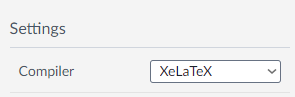
\includegraphics{IMAGE/Obraz1.png}
    \caption{Ustawienie kompilatora na platformie \overleaflink}
    
\end{figure}
Następnie należy wybrać z listy pilików \texttt{„Dyplom.tex”} i ustawić typ swojej pracy  w linii \textbackslash \texttt{documentclass} zmieniając \texttt{[thesis=inz]} na jedną z dostępnych opcji inz (praca inżynierska w języku polskim), mgr (praca magisterska w języku polskim), bsc (praca inżynierska w języku angielskim) lub msc (praca magisterka w języku angielskim). 
\begin{lstlisting}[caption={Ustawienia klasy dokumentu}, label=lst:Ustawienia klasy dokumentu, firstnumber=8]
\documentclass[thesis=inz]{TemplateCore/Dyplom}

 thesis=[inz|mgr|bsc|msc]
  * inz - praca inzynierska
  * mgr - praca magisterska
  * bsc - bachelor thesis
  * msc - master thesis
\end{lstlisting}
\clearpage
Poniżej znajduje się kolejna ważna opcja ponieważ wpływa ona na rodzaj sortowania bibliografii w wierszu 19 zmieniając \texttt{sorting=nty} na dostępne opcje: 
\begin{itemize}
\item[--] nty (Nazwisko, Tytuł, Rok),
\item[--] nyt (Nazwisko, Rok, Tytuł),
\item[--] none (Bez sortowania).
\end{itemize}
\begin{lstlisting}[caption={Ustawienia sortowania bibliografii}, label=lst:Ustawienia sortowania bibliografii, firstnumber=19]
	\usepackage[sorting=nty, bibfile=Dyplom]{TemplateCore/Dyplom} 
	
	- nty (Nazwisko, Tytul, Rok):
	- nyt (Nazwisko, Rok, Tytul):
	- none (Bez sortowania):
	 - nty (Author, Title, Year):
	 - nyt (Author, Year, Title):
	 - none (No sorting):

\end{lstlisting}
Nazwa pliku przy \texttt{bibfile=} powinna być zgodna z nazwą pliku naszej bibliografii u autora jest to plik \texttt{Dyplom.bib}
Po wybraniu odpowiednich opcji należy uzupełnić pola do personalizacji strony tytułowej zaczynające się w wierszu 28 pliku \texttt{Dyplom.tex}.
\begin{lstlisting}[caption={Ustawienia dotyczące strony tytułowej}, label=lst:Ustawienia dotyczące strony tytułowej ,firstnumber=28]
 Konfiguracja - do personalizacji
 Configuration - to be personalized

\kierunek{Informatyka}
\specjalnosc{Sieci}
\title{Szablom Pracy Dyplomowej}
\engtitle{Szablon Pracy Dyplomowej}
\album{99168}
\author{Wojciech Hyl}
\promotor{prof. dr hab. in\.z. Marcin Kowol}
\date{2023}
\longdate{2023-11-26}


\end{lstlisting}
\clearpage

W tym samym pliku po spersonalizowaniu należy napisać streszczenie w języku polskim jak i angielskim. Streszczenie  powinno zawierać minimum 100 znaków do maksymalnie 4000 i należy je napisać w formie streszczenia a nie spisu treści 
W kodzie poniżej użyto pakiet \texttt{lipsum}, który generuje fikcyjny, standardowy tekst.
\begin{lstlisting}[caption={Miejsce pisania streszczenia pracy}, label=lst:Miejsce pisania streszczenia pracy, firstnumber=47]

 Streszczenie pracy i abstract.
 Summary of the Thesis and Abstract

\streszczeniepracy{

	
	\lipsum[1-4]
}  koniec streszczenia

\slowakluczowe{A, B, C}

\thesisabstract{

	
	\lipsum[1-4]
}  end of abstract

\thesiskeywords{X, Y, Z}
\end{lstlisting}
\vspace{0.5cm}
Główna struktóra dokumentu została przedstawiona w listingu \ref{lst:Główna struktura dokumentu}
\begin{lstlisting}[caption={Główna struktura dokumentu}, label=lst:Główna struktura dokumentu]
% !TEX program = xelatex
% !TeX encoding = utf8
% !TeX spellcheck = pl-PL

% Wybierz rodzaj pracy dyplomowej 
% Pick thesis type 

\documentclass[thesis=inz]{TemplateCore/Dyplom}

% thesis=[inz|mgr|bsc|msc]
%  * inz - praca in\.zynierska
%  * mgr - praca magisterska
%  * bsc - bachelor thesis
%  * msc - master thesis

\usepackage[sorting=nty, bibfile=Dyplom]{TemplateCore/Dyplom} 

%- nty (Nazwisko, Tytul, Rok):
%- nyt (Nazwisko, Rok, Tytul):
%- none (Bez sortowania):
% - nty (Author, Title, Year):
% - nyt (Author, Year, Title):
% - none (No sorting):

%%%%%%%%%%%%%%%%%%%%%%%%%%%%%%%%%%%%%%%%%%%%%%%%%%%%%%%%%%%%%%%%%%%%%%%%%%%
% Konfiguracja - do personalizacji
% Configuration - to be personalized
%%%%%%%%%%%%%%%%%%%%%%%%%%%%%%%%%%%%%%%%%%%%%%%%%%%%%%%%%%%%%%%%%%%%%%%%%%%
\kierunek{Informatyka}
%\specjalnosc{Sieci}
\title{Szablon \LaTeX\ do pracy dyplomowej i prezentacji
}
\engtitle{Szablon \LaTeX\ do pracy dyplomowej i prezentacji
}
\album{99168}
\author{Wojciech Hyl}
\promotor{prof. dr hab. in\.z. Marcin Kowol}
\date{2023}
\longdate{2023-11-26}


%%%%%%%%%%%%%%%%%%%%%%%%%%%%%%%%%%%%%%%%%%%%%%%%%%%%%%%%%%%%%%%%%%%%%%%%%%%
% Streszczenie pracy i abstract.
% Summary of the Thesis and Abstract
%%%%%%%%%%%%%%%%%%%%%%%%%%%%%%%%%%%%%%%%%%%%%%%%%%%%%%%%%%%%%%%%%%%%%%%%%%%
\streszczeniepracy{
\lipsum[1-4]
} % koniec streszczenia

\slowakluczowe{Skład tekstu \LaTeX, Praca Dyplomowa, Narzędzia i środowiska pracy}

\thesisabstract{
\lipsum[1-4]
} % end of abstract

\thesiskeywords{Text Composition \LaTeX, Dissertation, Tools and working environments.}

%%%%%%%%%%%%%%%%%%%%%%%%%%%%%%%%%%%%%%%%%%%%%%%%%%%%%%%%%%%%%%%%%%%%%%%%%%%
% Tu zaczyna sie dokument
%%%%%%%%%%%%%%%%%%%%%%%%%%%%%%%%%%%%%%%%%%%%%%%%%%%%%%%%%%%%%%%%%%%%%%%%%%%
\begin{document}
	% Strony naglówkowe
	% Headers
	\frontpages
	
	% Wlasciwa tresc jest w pliku Chapters/main.tex
	% Real contents is in Chapters/main.tex
	
\chapter{Wprowadzenie}
\section{Wstęp}
W dzisiejszym globalnym świecie znajomość języków obcych jest nieocenioną umiejętnością. Tradycyjne metody nauki, takie jak lekcje w klasach, samouczki i aplikacje do nauki słownictwa, często są czasochłonne i nie zawsze dostosowane do indywidualnych potrzeb ucznia. Dodatkowo, oglądanie filmów i seriali w obcym języku jest powszechnie uznawane za skuteczny sposób na poprawę umiejętności językowych, ale brakuje narzędzi, które integrują te aktywności z formalnym procesem nauki. Niniejsza praca inżynierska koncentruje się na stworzeniu innowacyjnej aplikacji webowej, która połączy te dwa aspekty, oferując użytkownikom skuteczniejsze i przyjemniejsze doświadczenie edukacyjne.

Współczesny świat, w którym żyjemy, jest coraz bardziej zglobalizowany i wymaga od nas umiejętności komunikacji w różnych językach, a przede wszystkim w języku angielskim, który stał się międzynarodowym językiem na świecie. Wraz z rozwojem technologii, nauka języków obcych stała się bardziej dostępna i atrakcyjna. Znajomość języków obcych nie tylko otwiera drzwi do nowych możliwości zawodowych, ale także umożliwia pełniejsze zrozumienie innych kultur i poszerza horyzonty. Wraz z dynamicznym rozwojem technologii, nauka języków obcych stała się bardziej dostępna, a tradycyjne metody nauczania ewoluowały, oferując nowe, bardziej interaktywne formy edukacji. Jednym z najpopularniejszych sposobów nauki języków jest korzystanie z platform internetowych, takich jak duoLingo, gdzie użytkownicy mogą uczyć się od podstaw słów i zdań które zostały wcześniej przygotowane. Jednakże, nauka języka obcego w ten sposób ogranicza nas w kwesti wyboru czego chcielisbyśmy się dokładnie uczyć.

Coraz więcej osób szuka alternatywnych metod nauki, które są bardziej angażujące i interaktywne. Filmy i seriale oferują naturalny kontekst, w którym używane są różne zwroty i słownictwo, co czyni je doskonałym narzędziem do nauki języka. Oglądanie treści w języku obcym nie tylko pomaga w nauce nowych słów i zwrotów, ale także w poprawie umiejętności słuchania i rozumienia języka w różnych akcentach i dialektach.

Aplikacja ta ma umożliwić użytkownikom aktywne uczestnictwo w procesie nauki, poprzez interaktywne narzędzia i funkcje, które wspomagają naukę słownictwa i gramatyki. Wśród nich znajdują się m.in. możliwość zapisu słów z listy napisów, które są wyświetlane pod lub obok odtwarzacza video, a także możliwość dodania ich do bazy danych, aby uniknąć powtórzeń baza nie przyjmie drugiego takiego samego słowa użytkownikowi. Użytkownik będzie miał dostęp do panelu nauki, słownika wszystkich słów, możliwości logowania z różnych urządzeń obsługujących przeglądarkę, a także do różnych sposobów prezentacji danych, takich jak słownik, flashcards czy moduł do edycji napisów.

Aplikacja ta ma również uwzględnić elementy gamifikacji, aby zachęcić użytkowników do nauki i śledzenia postępów. Na profilu użytkownika będą widoczne wszystkie nauczone słowa, a także osobna podstrona z wykresami i informacjami o postępach. Dzięki tej aplikacji, użytkownicy będą mogli efektywnie i atrakcyjnie uczyć się języka obcego, korzystając z platformy YouTube i własnych filmów z napisami z dysku własnego komputera. Napisy których użytkownik może użyć będą w różnych formatach, więc w aplikacji będzię można wybrać rodzaj pliku i przekopiować całą zawartość lub wrzucić plik w odpowiednie miejsce, napisy muszą zostać zapisane w systemie ponieważ nie ma możliwośći zapisaniu scieżki do żadnego pliku ze względów bezpieczeństwa w internecie.

Wybór technologii do tworzenia aplikacji webowej jest kluczowy dla jej stabilności, skalowalności i wydajności. W projekcie tej aplikacji językowej zdecydowano się na framework Next.js, który oparty jest na React i oferuje wiele korzyści. Jedną z głównych zalet Next.js jest możliwość elastycznego renderowania treści, zarówno po stronie serwera (SSR), jak i klienta (CSR). Dzięki SSR, aplikacja może szybko ładować wstępnie załadowane strony, co znacząco poprawia widoczność w wyszukiwarkach (SEO - Search Engine Optimization) i przyspiesza czas ładowania, co jest szczególnie istotne dla użytkowników korzystających z platformy edukacyjnej. CSR z kolei umożliwia dynamiczne i płynne aktualizacje interfejsu bez konieczności przeładowywania całej strony, co poprawia doświadczenie użytkownika.


\section{Przegląd aktualnych rozwiązań}

\subsection{Anki}
Anki to popularna aplikacja edukacyjna oparta na systemie powtórek rozłożonych w czasie (Spaced Repetition System – SRS). Dzięki temu mechanizmowi nauka jest bardziej efektywna, ponieważ aplikacja prezentuje użytkownikowi informacje w odpowiednich odstępach czasowych, co pomaga w utrwaleniu materiału. Anki wyróżnia się uniwersalnością i możliwością dostosowania do różnych potrzeb, takich jak nauka języków obcych, przygotowanie do egzaminów czy zapamiętywanie faktów w innych dziedzinach.\\
\textbf{Funkcjonalności}:
\begin{itemize}
    \item Możliwość ręcznego dodawania kart z różnymi typami treści, w tym tekstów, obrazów, dźwięków i nagrań wideo.
    \item Obsługa dodatków (pluginów), które rozszerzają możliwości aplikacji, np. importowanie napisów filmowych.
    \item Analiza postępów użytkownika z wykorzystaniem statystyk i wykresów.
\end{itemize}
\textbf{Ograniczenia}:
\begin{itemize}
    \item Podczas oglądania filmu użytkownik musi ręcznie przerywać oglądanie, aby dodawać niezbędne informacje do kart. Utrudnia to płynność procesu i może obniżać komfort nauki.
    \item Mimo tych niedogodności Anki pozostaje dobrym rozwiązaniem do nauki języków, szczególnie dzięki możliwości personalizacji kart i śledzenia postępów.
\end{itemize}
\begin{figure}[H]
    \centering
    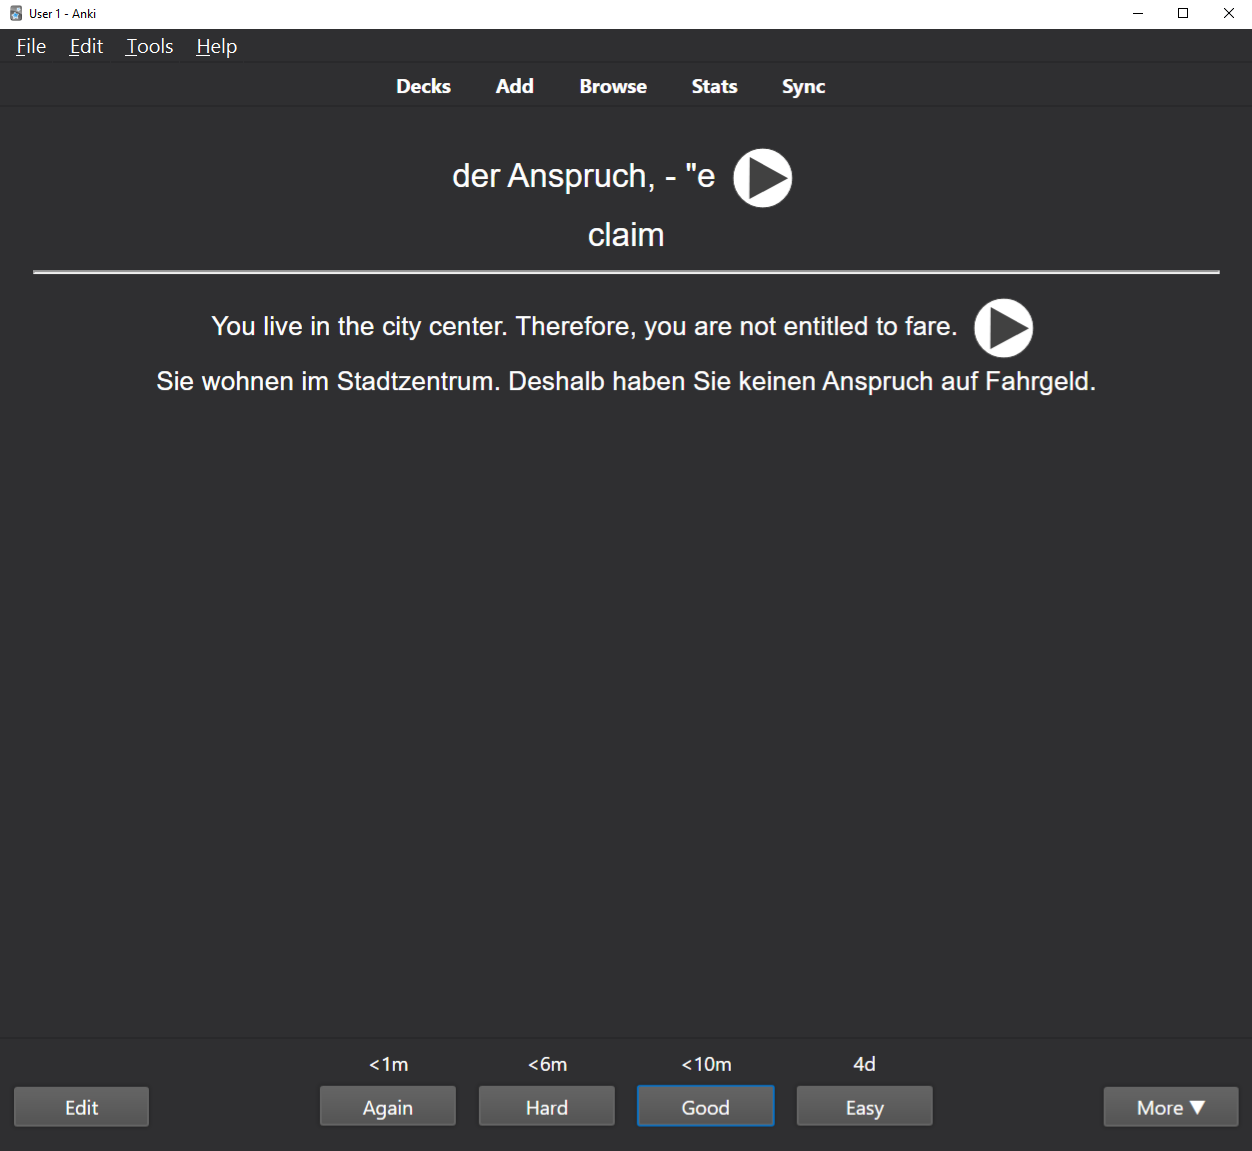
\includegraphics[width=0.8\textwidth]{IMAGE/Anki.png}
    \caption{Nauka słówek w aplikacji Anki}
    \label{fig:Anki}
\end{figure}
\subsection{Language Reactor}
Language Reactor to narzędzie edukacyjne, które umożliwia naukę języków obcych w sposób przyjemny i efektywny poprzez oglądanie filmów i seriali. Aplikacja oferuje interaktywne napisy, które umożliwiają tłumaczenie słów i zwrotów bezpośrednio na ekranie. Dzięki tej funkcji użytkownicy mogą szybko sprawdzić znaczenie nowego słowa, klikając na nie podczas oglądania, lub oznaczyć jako słowo do nauki, ale jest to możliwe dopiero po zapłaceniu za usługę “pro” na stronie. \\
\textbf{Funkcjonalności}:
\begin{itemize}
    \item {\textbf{Interaktywne napisy}}: Jedną z głównych zalet Language Reactor jest możliwość wyświetlania tłumaczeń słów i zwrotów w trakcie oglądania, co sprawia, że nauka odbywa się w naturalnym kontekście. Dzięki temu użytkownik może natychmiast zobaczyć, jak dane słowo funkcjonuje w zdaniu.
    \item {\textbf{Integracja z platformami streamingowymi}}: Aplikacja działa z popularnymi serwisami, takimi jak YouTube, Netflix czy Disney+, co oznacza, że użytkownicy mogą korzystać z niej podczas oglądania ulubionych filmów i seriali w obcym języku.
    \item {\textbf{Słownik i lematyzacja}}: Language Reactor automatycznie przetwarza słowa na ich formy podstawowe (lematy), co pomaga w nauce gramatyki oraz zapamiętywaniu nowych słówek bez względu na ich odmianę.
    \item {\textbf{Baza słówek}}: Użytkownicy mogą zapisywać słówka, które napotkali podczas oglądania, tworząc spersonalizowaną listę do późniejszego przyswajania. To rozwiązanie pozwala na systematyczną naukę i powtórki.
    \item {\textbf{System powtórek SRS}}: Aplikacja wprowadza system powtórek rozłożonych w czasie, co wspomaga długotrwałe zapamiętywanie materiału, podobnie jak w przypadku Anki.
    \item {\textbf{ifDostosowanie poziomu trudności}}: Użytkownicy mogą dostosować poziom trudności materiałów, co pozwala na naukę dostosowaną do ich umiejętności i tempa.
\end{itemize}

\textbf{Ograniczenia}:
\begin{itemize}
    \item \textbf{Ograniczona dostępność}: Language Reactor jest dostępny tylko na wybranych platformach streamingowych, co ogranicza możliwość korzystania z aplikacji do nauki języków z innych źródeł.
    \item \textbf{Płatne funkcje}: Pełna funkcjonalność aplikacji, w tym możliwość zapisywania słówek i korzystania z systemu powtórek, jest dostępna tylko w wersji płatnej, co może być barierą dla niektórych użytkowników.
\end{itemize}

\begin{figure}[H]
    \centering
    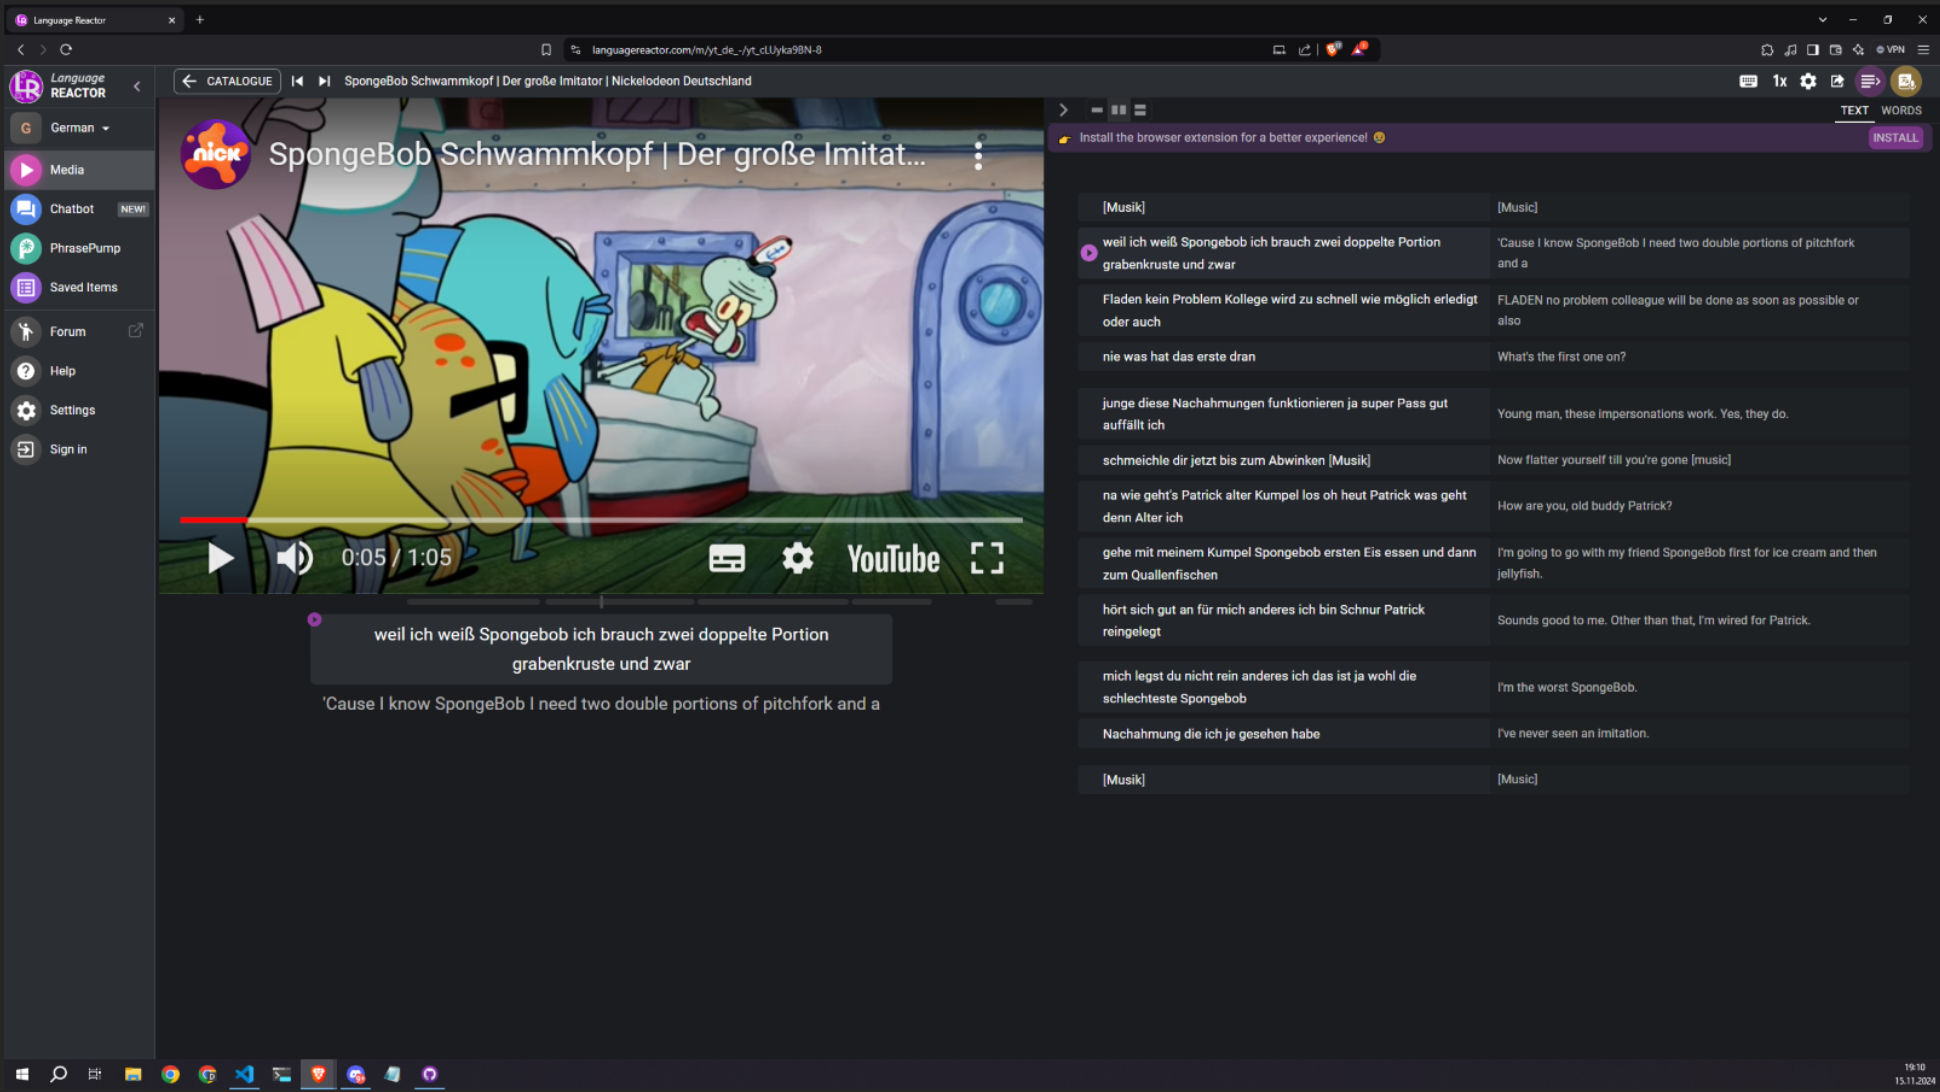
\includegraphics[width=0.8\textwidth]{IMAGE/LanguageReactor.png}
    \caption{Interaktywne napisy na stronie Language Reactor}
    \label{fig:Language_reactor}
\end{figure}

Możliwość nauki tylko z wybranych kanałów youtube nie można wybrać filmu który nie jest na liście strony internetowej.
\subsection{Trancy}
Trancy to aplikacja stworzona z myślą o nauce języków obcych, która integruje naukę słówek z oglądaniem filmów, seriali i innych materiałów wideo. Aplikacja oferuje funkcje, które pozwalają użytkownikom uczyć się języka poprzez interaktywne napisy, tłumaczenia oraz dodatkowe ćwiczenia, co sprawia, że proces nauki staje się bardziej angażujący i efektywny. \\
\textbf{Funkcjonalności}:
\begin{itemize}
    \item \textbf{Interaktywne napisy}: Trancy umożliwia wyświetlanie napisów w różnych językach, z tłumaczeniami słów i zwrotów. Dzięki temu użytkownicy mogą szybko zrozumieć, co oznacza dane słowo, a także zobaczyć je w kontekście. Napisy są dostosowane do poziomu zaawansowania użytkownika, co pozwala na naukę w sposób dostosowany do indywidualnych potrzeb.
    \item \textbf{Zbieranie słówek}: Użytkownicy mogą zapisywać napotkane słówka, które następnie mogą zostać przekształcone w fiszki do nauki. Taki system pozwala na systematyczne utrwalanie materiału i umożliwia szybkie powtórki w dogodnym czasie.
    \item \textbf{Tłumaczenia i definicje}: Aplikacja oferuje tłumaczenie słów na różne języki oraz wyświetlanie ich definicji, co wspomaga naukę gramatyki i budowanie słownictwa. Użytkownicy mogą korzystać z wbudowanego słownika, aby na bieżąco zgłębiać znaczenie nowych wyrazów.
    \item \textbf{Fiszki SRS}: Trancy wykorzystuje system powtórek rozłożonych w czasie (SRS), który pomaga w długotrwałym zapamiętywaniu słówek. Użytkownik dostaje powiadomienia o konieczności powtórki, co pozwala na regularne utrwalanie materiału i skuteczniejszą naukę.
\end{itemize}
\textbf{Ograniczenia}:
\begin{itemize}
    \item \textbf{Wymaga płatnej subskrypcji}: Aby w pełni skorzystać z funkcji aplikacji, użytkownik musi zapłacić, w wersji darmowej są tylko niezbędne narzędzia jak tłumaczenie i limit do 100 słów do zapisania.
    \item \textbf{Ograniczona integracja z platformami}: Trancy oferuje integrację z wybranymi platformami streamingowymi, i nie daje możliwości nauki z własnych zapisanych filmów.
    \item \textbf{Wymagana wtyczka w przeglądarce}: Żeby dodawać słowa lub oglądać filmy musimy robić to poza stroną Trancy z użyciem wtyczki Trancy.
\end{itemize}

\begin{figure}[H]
    \centering
    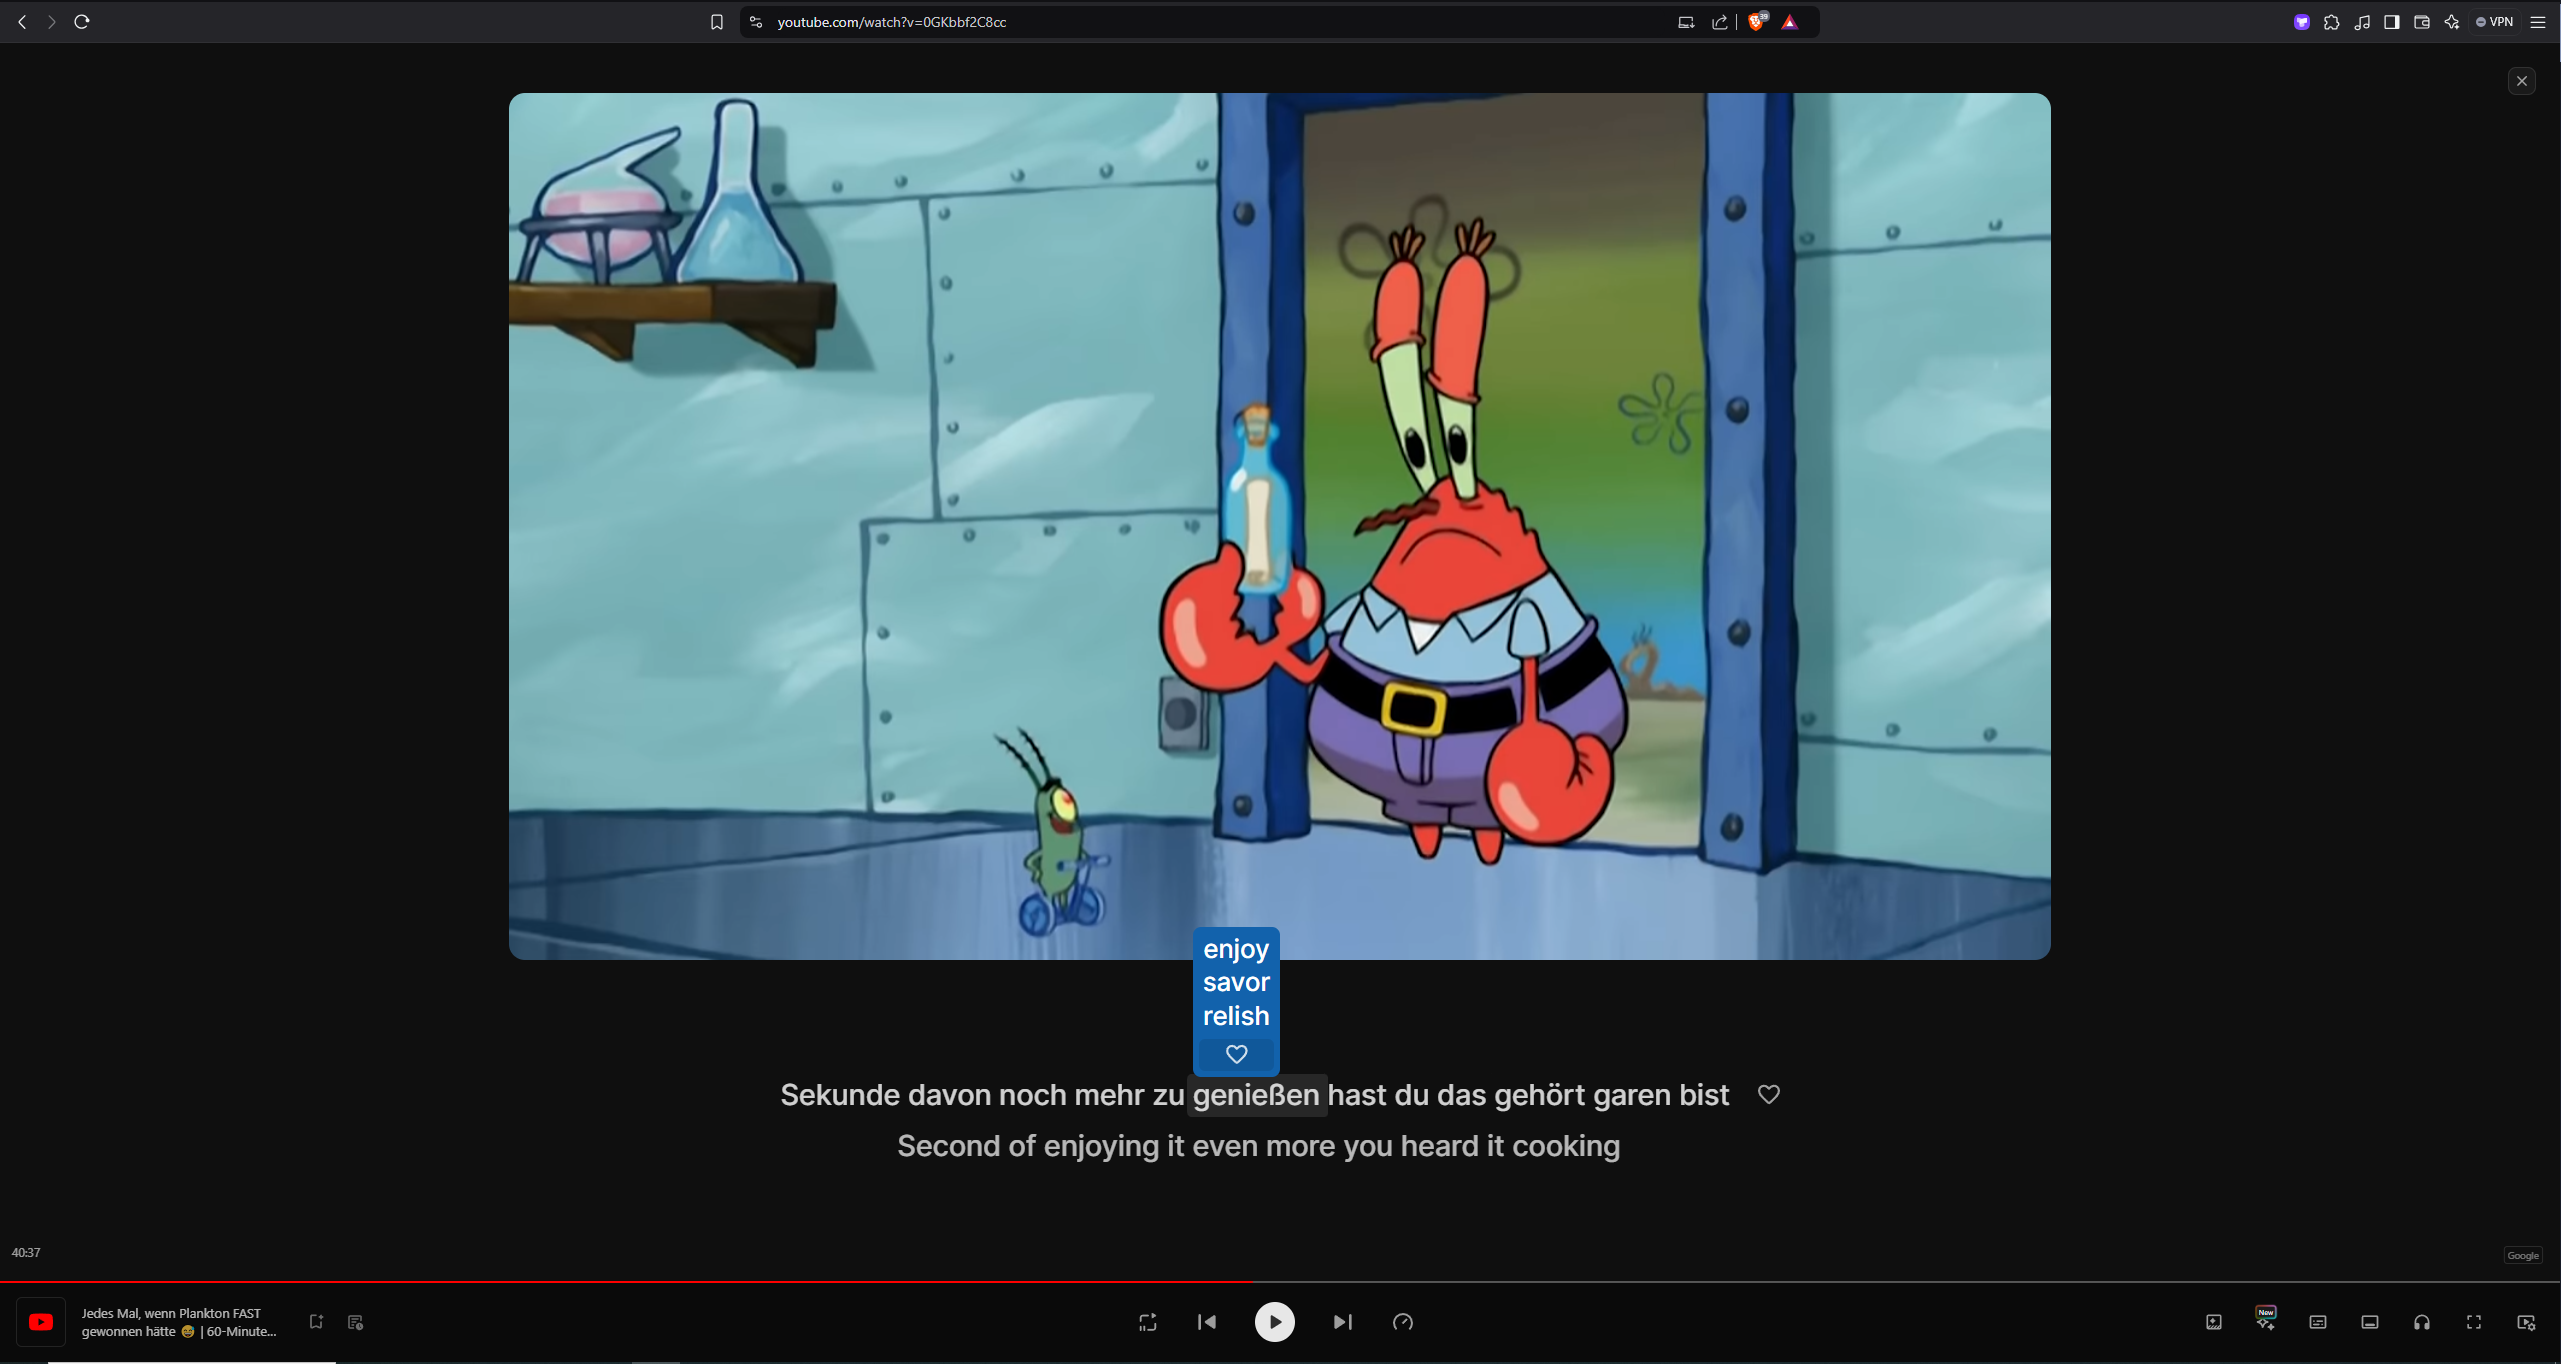
\includegraphics[width=0.8\textwidth]{IMAGE/Trancy.png}
    \caption{Interaktywne napisy Trancy}
    \label{fig:Trancy}
\end{figure}

\chapter{Cel i zakres pracy}
\section{Cel pracy}
Głównym celem niniejszej pracy jest zaprojektowanie i implementacja aplikacji webowej wspomagającej naukę języków obcych poprzez oglądanie filmów i seriali. Aplikacja ma umożliwiać użytkownikom naukę wybranego języka obcego podczas oglądania treści multimedialnych własnego wyboru. Główne założenia to:

\begin{enumerate}
    \item \textbf{Łatwość w nauce}: Umożliwienie użytkownikom nauki języków poprzez napisy w filmach i serialach
          bez potrzeby tworzenia kart do nauki w innych aplikacjach,
          takich jak Anki oszczędzając przy tym dużo czasu użytkownika.
    \item \textbf{Połączenie nauki z rozrywką}: Użytkownicy będą mogli uczyć się języka podczas oglądania swoich ulubionych filmów i seriali,
          co czyni naukę bardziej przyjemną i efektowną.
    \item \textbf{Baza danych}: Umożliwienie użytkownikom zapisywania trudnych słów do bazy danych,
          unikając duplikacji słów za pomocą blokady w bazie danych do wyciągnięcia z tego 100\% skuteczności pomagać będzie lematyzacja słów,
          czyli proces upraszczania słowa do jego formy słownikowej.
    \item \textbf{Spersonalizowane środowisko nauki}: Dostęp do panelu użytkownika z podsumowaniem postępów w nauce,
          różnorodne metody nauki słownictwa i gramatyki (fiszki, quizy, gry edukacyjne),
          możliwość śledzenia statystyk i wykresów przedstawiających postępy w nauce,
          a także gamifikacja procesu nauki poprzez nagradzanie użytkowników za osiągnięcia.
    \item \textbf{Różne sposoby nauki}: Wgląd do danych za pomocą różnych metod jak flashcards, moduł do edycji napisów, quiz, wpisywania tłumaczenia słowa itp.
    \item \textbf{Motywacja i śledzenie postępów}: Aplikacja będzie motywować użytkowników do nauki poprzez wizualizację ich postępów za pomocą statystyk, wykresów i informacji widocznych na profilu użytkownika.
    \item \textbf{Zapewnienie kompatybilności}: Aplikacja bedzie dostępna z różnych przeglądarek internetowymi i urządzeń.
    \item \textbf{Innowacyjne rozwiązania technologiczne}: Wykorzystanie sztucznej inteligencji do tłumaczenia napisów i ich przetwarzanie przy użyciu NLP,
          oraz zastosowanie nowoczesnych technologii webowych do zapewnienia płynnego działania aplikacji.
\end{enumerate}

\section{Zakres pracy}
Zakres pracy obejmuje szczegółowe opisanie i realizację następujących etapów:

\begin{itemize}
    \item \textbf{Opracowanie architektury systemu}.
    \item \textbf{Projektowanie i implementacja bazy danych}.
    \item \textbf{Tworzenie logiki aplikacji oraz jej frontendu i backendu}.
    \item \textbf{Zabezpieczenie aplikacji przed redundancją danych oraz niepoprawnymi wpisami}.
    \item \textbf{Umożliwienie użytkownikom logowania z różnych urządzeń obsługujących przeglądarki}.
    \item \textbf{Implementacja różnych metod nauki (słownik, flashcards, edycja napisów) oraz elementów gamifikacji}.
\end{itemize}
Na rynku dostępne są różne aplikacje wspomagające naukę języków obcych, takie jak Duolingo, Anki, Quizlet, Memrise, Babbel, Rosetta Stone, LingQ, FluentU, Clozemaster, itp.
\section{Przegląd aktualnych rozwiązań}

\subsection{Anki}
Anki to popularna aplikacja edukacyjna oparta na systemie powtórek rozłożonych w czasie (Spaced Repetition System – SRS). Dzięki temu mechanizmowi nauka jest bardziej efektywna, ponieważ aplikacja prezentuje użytkownikowi informacje w odpowiednich odstępach czasowych, co pomaga w utrwaleniu materiału. Anki wyróżnia się uniwersalnością i możliwością dostosowania do różnych potrzeb, takich jak nauka języków obcych, przygotowanie do egzaminów czy zapamiętywanie faktów w innych dziedzinach. \\
\textbf{Funkcjonalności}:
\begin{itemize}
    \item Możliwość ręcznego dodawania kart z różnymi typami treści, w tym tekstów, obrazów, dźwięków i nagrań wideo.
    \item Obsługa dodatków (pluginów), które rozszerzają możliwości aplikacji, np. importowanie napisów filmowych.
    \item Analiza postępów użytkownika z wykorzystaniem statystyk i wykresów.
\end{itemize}
\textbf{Ograniczenia}: \\
Podczas oglądania filmu użytkownik musi ręcznie przerywać oglądanie, aby dodawać niezbędne informacje do kart. Utrudnia to płynność procesu i może obniżać komfort nauki. Mimo tych niedogodności Anki pozostaje dobrym rozwiązaniem do nauki języków, szczególnie dzięki możliwości personalizacji kart i śledzenia postępów.

\subsection{Language Reactor }
Language Reactor to narzędzie edukacyjne, które umożliwia naukę języków obcych w sposób przyjemny i efektywny poprzez oglądanie filmów i seriali. Aplikacja oferuje interaktywne napisy, które umożliwiają tłumaczenie słów i zwrotów bezpośrednio na ekranie. Dzięki tej funkcji użytkownicy mogą szybko sprawdzić znaczenie nowego słowa, klikając na nie podczas oglądania, lub oznaczyć jako słowo do nauki, ale jest to możliwe dopiero po zapłaceniu za usługę “pro” na stronie. \\
\textbf{Funkcjonalności}:
\begin{itemize}
    \item {\textbf{Interaktywne napisy}}: Jedną z głównych zalet Language Reactor jest możliwość wyświetlania tłumaczeń słów i zwrotów w trakcie oglądania, co sprawia, że nauka odbywa się w naturalnym kontekście. Dzięki temu użytkownik może natychmiast zobaczyć, jak dane słowo funkcjonuje w zdaniu.
    \item {\textbf{Integracja z platformami streamingowymi}}: Aplikacja działa z popularnymi serwisami, takimi jak YouTube, Netflix czy Disney+, co oznacza, że użytkownicy mogą korzystać z niej podczas oglądania ulubionych filmów i seriali w obcym języku.
    \item {\textbf{Słownik i lematyzacja}}: Language Reactor automatycznie przetwarza słowa na ich formy podstawowe (lematy), co pomaga w nauce gramatyki oraz zapamiętywaniu nowych słówek bez względu na ich odmianę.
    \item {\textbf{Baza słówek}}: Użytkownicy mogą zapisywać słówka, które napotkali podczas oglądania, tworząc spersonalizowaną listę do późniejszego przyswajania. To rozwiązanie pozwala na systematyczną naukę i powtórki.
    \item {\textbf{System powtórek SRS}}: Aplikacja wprowadza system powtórek rozłożonych w czasie, co wspomaga długotrwałe zapamiętywanie materiału, podobnie jak w przypadku Anki.
    \item {\textbf{ifDostosowanie poziomu trudności}}: Użytkownicy mogą dostosować poziom trudności materiałów, co pozwala na naukę dostosowaną do ich umiejętności i tempa.
\end{itemize}
\textbf{Ograniczenia}: \\
Płatna subskrypcja daje nam możliwość nauki na stronie, bezpłatnie możemy tylko zobaczyć film z przetłumaczonymi napisami.

Możliwość nauki tylko z wybranych kanałów youtube nie można wybrać filmu który nie jest na liście strony internetowej.
\subsection{Trancy}
Trancy to aplikacja stworzona z myślą o nauce języków obcych, która integruje naukę słówek z oglądaniem filmów, seriali i innych materiałów wideo. Aplikacja oferuje funkcje, które pozwalają użytkownikom uczyć się języka poprzez interaktywne napisy, tłumaczenia oraz dodatkowe ćwiczenia, co sprawia, że proces nauki staje się bardziej angażujący i efektywny. \\
\textbf{Funkcjonalności}:
\begin{itemize}
    \item \textbf{Interaktywne napisy}: Trancy umożliwia wyświetlanie napisów w różnych językach, z tłumaczeniami słów i zwrotów. Dzięki temu użytkownicy mogą szybko zrozumieć, co oznacza dane słowo, a także zobaczyć je w kontekście. Napisy są dostosowane do poziomu zaawansowania użytkownika, co pozwala na naukę w sposób dostosowany do indywidualnych potrzeb.
    \item \textbf{Zbieranie słówek}: Użytkownicy mogą zapisywać napotkane słówka, które następnie mogą zostać przekształcone w fiszki do nauki. Taki system pozwala na systematyczne utrwalanie materiału i umożliwia szybkie powtórki w dogodnym czasie.
    \item \textbf{Tłumaczenia i definicje}: Aplikacja oferuje tłumaczenie słów na różne języki oraz wyświetlanie ich definicji, co wspomaga naukę gramatyki i budowanie słownictwa. Użytkownicy mogą korzystać z wbudowanego słownika, aby na bieżąco zgłębiać znaczenie nowych wyrazów.
    \item \textbf{Fiszki SRS}: Trancy wykorzystuje system powtórek rozłożonych w czasie (SRS), który pomaga w długotrwałym zapamiętywaniu słówek. Użytkownik dostaje powiadomienia o konieczności powtórki, co pozwala na regularne utrwalanie materiału i skuteczniejszą naukę.
\end{itemize}
\textbf{Ograniczenia}:
\begin{itemize}
    \item \textbf{Wymaga płatnej subskrypcji}: Aby w pełni skorzystać z funkcji aplikacji, użytkownik musi zapłacić, w wersji darmowej są tylko niezbędne narzędzia jak tłumaczenie i limit do 100 słów do zapisania.
    \item \textbf{Ograniczona integracja z platformami}: Trancy oferuje integrację z wybranymi platformami streamingowymi, i nie daje możliwości nauki z własnych zapisanych filmów.
    \item \textbf{Wymagana wtyczka w przeglądarce}: Żeby dodawać słowa lub oglądać filmy musimy robić to poza stroną Trancy z użyciem wtyczki Trancy.
\end{itemize}

\chapter{Opis technologii}


Struktura dokumentów \LaTeX\ przedstawiona w listingu \ref{lst:Przykład prostego dokumentu} obejmuje proste i podstawowe polecenia. Dokumenty \LaTeX\ zaczynamy od \textbf{preambuły} która znajdująca się przed właściwą treścią dokumentu. Preambuła zawiera instrukcje i ustawienia, które wpływają na cały dokument. Najczęściej zawiera takie inforamcje jak: klasa dokumentu, ustawienia strony czy pakiety. W przypadku podanego przykładu zaczynamy od wyboru klasy którym jest \texttt{article}, więcej informacji na temat wyboru klas w dokumentach \LaTeX\ można znaleźć w podrozdziale \ref{sec:klassa}. Następnym elementem są pakiety w \LaTeX\ to zestawy makr i definicji, które rozszerzają funkcjonalność języka \LaTeX\. Dzięki pakietom możesz dostosować formatowanie, dodawać nowe polecenia czy obsługiwać specjalne elementy, takie jak tabelki, grafika czy dodatkowe czcionki. Wczytujemy pakietu w \LaTeX\ za pomocą polecenie \texttt{\textbackslash usepackage{\{Nazwa\textunderscore pakietu\}}} jednak należy pamiętać że niektóre pakiety mogą wchodzić z sobą w konflikt. Kolejnym elementem przedstawionym w listingu \ref{lst:Przykład prostego dokumentu} jest makro to niestandardowe polecenia, które można definiować i używać w celu skrócenia i uproszczenia kodu. Makra pozwalają na zdefiniowanie własnych komend, które mogą być używane w dokumencie. Mogą być one przydatne, gdy chcemy wielokrotnie używać tego samego fragmentu kodu, lub gdy chcemy nadać bardziej znaczącą nazwę bardziej skomplikowanym lub długim sekwencjom poleceń. W przedstawionym przykładzie zostało stworzone makro wstawiającą hiperłącze do platformy Overleaf. Kolejnym elementem są metadane dokumentu to informacje charakteryzujące sam dokument, takie jak tytuł, autor, data itp. Ostatnim elementem w przedstawionym przykładzie jest właściwa treść dokumentu która nie jest już częścią preambuły zaczyna się od \texttt{\textbackslash begin\{document\}} a kończy na \texttt{\textbackslash end\{document\}} wszystkie elementy zawarte pomiędzy tworzą treść. Element \texttt{\textbackslash maketitle} generuje stronę tytułową na podstawie zdefiniowanych metadanych. Za pomocą komendy \texttt{\textbackslash section\{Nazwa\textunderscore sekcji\}} tworzona jest nową sekcje w naszym dokumencie.
\clearpage 
\begin{lstlisting}[caption={Przykład prostego dokumentu}, label=lst:Przykład prostego dokumentu]
\documentclass{article}

% \usepackage[utf8]{inputenc}  % Kodowanie znaków 
\usepackage[T1]{fontenc}     % Kodowanie fontu
\usepackage[polish]{babel}   % J?zyk dokumentu
\usepackage{graphicx}        % Obsługa grafiki
\usepackage{hyperref}        % Dodanie pakietu do obsługi hiperłączy

% Makro
\newcommand{\overleaflink}{\href{https://www.overleaf.com/}{Overleaf }}

\title{Przykładowy Dokument w LaTeX}
\author{Wojtek Hyl}
\date{\today}

\begin{document}
	
	\maketitle
	
	\section{Wprowadzenie}
	Tutaj możesz opisać wprowadzenie do swojego dokumentu.
	
	\section{Link do Overleaf}
	Korzystając z makra, możesz wstawić hiperłącze do Overleaf: \overleaflink
	
\end{document}

\end{lstlisting}



\overleaflink to platforma internetowa umożliwiająca pracę z dokumentami \LaTeX, która ułatwia autorom pisanie i formatowanie tekstów naukowych. Platforma oferuje również dostęp do szablonów udostępnionych przez użytkowników. Dzięki temu, że jest to platforma online nie ma potrzeby instalowania żadnych dodatkowych programów na lokalnym komputerze. Ułatwia to dostępność i pracę z dowolnego miejsca z dostępem do internetu. Możliwość pracy online umożliwia pracę w zespołach nad jednym dokumentem w czasie rzeczywistym co jest bardzo ważnym elementem. \overleaflink umożliwia integracje z platformą GitHub, co umożliwia przechowywanie dokumentów \LaTeX w systemie kontroli wersji. Ułatwia to przechowywanie wersji projektu, śledzenie zmian oraz współpracę z innymi programistami. \overleaflink oferuje również integracje z Dropboxem która umożliwia przechowywania i synchronizacje plików w chmurze. Dropbox jest bardziej intuicyjnym narzędziem do przechowywania kodów niż GitHub jednakże nie posiada kontroli wersji. Platforma oferuje bogaty zasób funkcji takich jak na przykład natychmiastowy podgląd, sprawdzanie poprawności kodu, sugestie poprawek i wiele inny przydatnych funkcjonalności. Dodatkowo strona obsługuje wiele języków, co umożliwia pisanie oraz formatowanie w wybranym języku. Bibliografia na platformie jest zintegrowana z systemem zarządzania bibliografią. Pomaga to w generowaniu bibliografii z wybranym stylem. Posiada integracje z takim portalami jak Mendeley i Zotero, co umożliwia importowanie i eksportowanie bibliografii w różnych formatach, a także pozwala na integrację z zarządzaniem referencjami. \overleaflink oferuje także bardzo bogatą i łatwo dostępną dokumentacje oraz instrukcję obsługi pakietów. Podsumowując platforma ułatwia tworzenie dokumentów \LaTeX dla osób, które nie chcą instalować żadnego dodatkowego oprogramowania swoim komputerze lokalnym i chcą mieć dostęp do swoich dokumentów w każdym miejscu. Jest również świetnym narzędziem do pracy w zespołach które pracują online nad swoimi dokumentami. Należy jednak pamiętać że takie funkcje jak integracja z GitHubem, DropBoxem, Mendeley i Zotero są wyłącznie dostępne w płatnej subskrypcji \overleaflink. Płatna wersja również zawiera wsparcie priorytetowe (ang. priority support) co umożliwia szybsze wsparcie z strony \overleaflink w razie problemów.  

\LaTeX\ umożliwia również pracę w środowisku lokalnym. Istnieje wiele narzędzi używanych do tworzenia, kompilowania i zarządzania dokumentami \LaTeX. Jedną z istotniejszych narzędzi jakie są potrzebne to edytory. Do najczęściej używanych zaliczamy TeXShop, TeXworks i TeXstudio. Edytor TeXShop umożliwiający pracę z \LaTeX{em} na systemy OS X. Posiada prosty interfejs i jest łatwy w użyciu. Natomiast jeżeli chodzi o edytory dostępne na wielu systemach możemy do nich zaliczyć TeXworks i TeXstudio. Kolejną ważna rzeczą jaka jest potrzebna do używania \LaTeX{a} na komputerach lokalnych jest jego dystrybucja. Do najczęściej używanych dystrybucji należą TeX Live i MiKTex. TeX Live jest to dystrybucja \LaTeX\ dostępna na wielu platformach obejmująca pełen zestaw pakietów i narzędzi. MikTex jest dystrybucją \LaTeX\ przeznaczoną dla systemów Windows podobnie jak Tex Live zawiera pełen zestaw pakietów i narzędzi. Ostatnią rzeczą jaka jest potrzebna do pracy z \LaTeX{em} jest kompilator. pdf\LaTeX\ jest najczęściej używanym kompilatorem umożliwiającym bezpośrednio generację plików PDF. Obsługuje nowoczesne funkcje, takie jak przykład na hiperłącza, wbudowane obrazy oraz obsługę różnych fontów. Jednym z kolejnych kompilatorów jest Xe\LaTeX. Obsługuje on fonty systemowe co umożliwia użycie innych fontów niż standardowe w \LaTeX. Obsługuje również Unicode, co pozwala na pracę w wielu językach i kodowań znaków. LuaLa\TeX\ jest edytorem umożliwiające zaawansowane operacje programistyczne używające silnika Lua\TeX\ jest rozwinięciem pdf\LaTeX. 


\chapter{Usprawnienie formatowania i estetyki}

\section{Marginesy i układ strony }\label{sec:klassa}
W szablonach \LaTeX\ ustawienia dotyczące marginesów i układu strony są kluczowe, ponieważ wpływają na końcowy wygląd dokumentu. Jednym z ważniejszych rzeczy jest odpowiedni wybór klasy dokumentu, która jest zgodna z wymaganiami. Każda klasa ma swoje specyficzne cechy i ustawienia, które można edytować do indywidualnych potrzeb. Do najczęściej używanych klas należą \texttt{article}, \texttt{report} czy \texttt{letter}. O właściwościach klas można się dowiedzieć czytając informacje na ich temat w rozdziale 8 książki ~\cite{diller2001latex}. \LaTeX\ umożliwia ustawianie układu strony do własnych potrzeb. Ustawianie marginesów jest ważnym elementem w kontekście estetyki. Do ustawiania marginesów w \LaTeX\ służy pakiet \texttt{geometry}, który umożliwia ich dokładnie ustawianie. Marginesy w ogólnym przypadku określają pustą przestrzeń między kolumną tekstu a krawędziami strony. Właściwie dostosowane wpływają na estetykę i ogólny odbiór dokumentu. W większości przypadków, np. w pracy dyplomowej ich wartość ustawia się zazwyczaj na 2,5 cm. Jeśli chodzi o \LaTeX\ wartości marginesów można ustawić za pomocą wspomnianego wyżej przedstawionego pakietu \texttt{geometry}. Domyślne ustawienia zależą jednak od wybranej klasy dokumentu, jednak bardzo łatwo można dostosować ich wartość do własnych potrzeb. 

Kolejnym elementem w kontekście formatowania i estetyki jest określenie czy dokument ma być jednostronny czy dwustronny. Ważne jest to o tyle, że dla dokumentów dwustronnych mogą występować różnice, jeśli chodzi o numeracje stron i marginesy, jeśli chodzi o strony parzyste czy nieparzyste. W układzie dwustronnym, dostosowanie numeracji stron jest istotne, aby zachować spójność i estetykę wizualną. Często stosuje się różne układy numeracji stron na stronach lewych i prawych, a także dostosowuje ich położenie, na przykład umieszczając numerację stron na środku strony. Określenie pionowej i poziomej justyfikacji wspomaga pakiet \texttt{ragged2e}. Pozwala on na elastyczniejszą justyfikację tekstu w obrębie tych kierunków. \LaTeX\ pozwala również na określenie innych parametrów takie jak rozmiar papieru, odstęp między tekstem a nagłówkiem czy też między stopką a tekstem. Ważne jest, aby dostosować te wartości do własnych preferencji czy też określonych wymagań. Odpowiednie przystosowanie tych elementów pozwala na stworzenie dokumentu o elastycznym układzie. Gwarantuje to również profesjonalny wygląd a sam dokument staje się bardziej przyjemny w odbiorze.  

\section{Czcionka i interlinia}
Elementy takie jak czcionka i interlinia wpływają drastycznie na wygląd dokumentu, ponieważ źle wybrany font tekstu czy odstęp pomiędzy wierszami utrudniają czytelność i pogarszają wygląd dokumentu. Czcionkę dostosowujemy przy użyciu pakietu \texttt{fontspace}. Jednak trzeba pamiętać, że nie wszystkie fonty są dostępne w domyślniej wersji systemu, więc używanie niestandardowych wymaga ich dodania za pomocą pakietu \texttt{fontspec}. Interlinię w \LaTeX\ możemy dostosowywać za pomocą pakietu takiego jak \texttt{setspace}. Ustawienie odstępu między wierszami na 1 będzie skutkowało tym, że odstęp będzie równy wysokości czcionki. Analogicznie ustawienie go na 2 będzie zwiększało go dwukrotnie. W stworzony przez autora szablonie została użyta czcionka \texttt{Latin Modern Roman} która jest główną krojem pisma. Natomiast  czcionka \texttt{Latin Modern Math} została zastosowana do wzorów matematycznych. 

\section{Nagłówki i stopki}
Nagłówki i stopki w \LaTeX\ są obsługiwanie przez na przykład pakiet \texttt{fancyhdr}. Pakiet umożliwia regulację górnych (nagłówki) i dolnych (stopy) elementów każdej strony. Oferuje on możliwość dostosowywania takich elementów jak na przykład linie oddzielające od treści, odległości, numerację stron i umieszczanie nazw rozdziałów. Umożliwia także ustawianie różnych wyglądów stopki i nagłówka dla stron parzystych i nieparzystych. Ważnie jest, aby dostosowywać te elementy do potrzeb własnej pracy.

\section{Numeracja rozdziałów i sekcji}
Numeracja rozdziałów i sekcji jest automatycznie prowadzona, jednakże jest możliwość dostosowania w jaki sposób te numery są formatowane czy które struktury mają być numerowane. Domyślnie każdy rozdział jest przedstawiony w formie numeru rozdziału przed jego tytułem. \LaTeX\ za pomocą pakietu \texttt{titlesec} umożliwia zmienianie formy wyświetlania. Sekcje podobnie jak rozdziały są numerowane. Automatycznie możemy kontrolować, które sekcje są numerowa za pomocą komendy \texttt{setcounter}, jednak należy pamiętać, że nienumerowane sekcje nie pojawią się w spisie treści. Pakiet \texttt{titlesec} również umożliwia kontrolę i edycje sekcji. Warto mieć na uwadze, że zbyt duża ilość numeracji poziomów może zmniejszać czytelność dokumentu i profesjonalny wygląd. 

\section{Rozmieszczenie grafik i tabel}
W wielu dokumentach grafiki są istotnym elementem przedstawienia treści. Pakiet \texttt{graphicx} jest narzędzie dodające możliwość wstawiania grafik w \LaTeX. Otoczenie  \texttt{figure} pozwala na umieszczanie grafiki, a także umożliwia również kontrole i numerację wstawionej treści w dokumencie. Umieszczone w ten sposób grafiki automatycznie są podpisywane i opisywane, a sam spis grafik jest generowany w sposób zautomatyzowany. Kolejnym istotnym elementem przedstawiania treści w \LaTeX\ są tabele. Dzięki otoczeniu \texttt{table} istnieje precyzyjna kontrola ich położenia oraz numeracja, podobnie jak w środowisku \texttt{figure}. Spis tabel jest generowany automatycznie i może być wstawiony w dowolnym miejscu w dokumencie. Istnieje wiele edytorów internetowych które ułatwiają tworzenie tabel dla osób, które nie są zaznajomione z \LaTeX{em} lub preferują wizualne interfejsy do projektowania tabel. Pozwalają one generować kod \LaTeX\ bez konieczności ręcznego wpisywania skomplikowanych komend. Rozmieszczenie grafik i tabel wymaga dobrego poznania struktury i użycia odpowiednich środowisk. Więcej na temat użycia otoczenia \texttt{figure} w podrozdziale \ref{sec:grafika} i na temat otoczenia \texttt{table} w podrozdziale \ref{sec:tabel}. Informacji na temat mechanizmu umiejscawiania obiektów ruchomych można znaleźć np. w podrozdziale 2.11 publikacji \cite{oetiker2022nie} lub podrozdziale 8.4.1 książki \cite{kucharczyk1994wprowadzenie}. Ważnym elementem jest zadbanie o odpowiednie podpisy co znacząco ułatwia nawigację po dokumencie. 

\section{Kolory i formatowanie}
\LaTeX\ jest narzędziem umożliwiającym dostosowywanie koloru tekstu do potrzeb dokumentu. Pakietem umożliwiający kontrolę nad kolorem jest \texttt{xcolor}. Dzięki temu pakietowi można dostosować kolor tekstu i tła. Obsługuje kolory podawane po nazwie, RGB , HTML, CMYK i szaro-skali. Stosowanie kolorów w dokumentach czy prezentacjach daje możliwość podkreślenia ważnych elementów, poprawia czytelność i zrozumiałość,  a w prezentacjach poprawia atrakcyjność wizualną pracy. Jednakże pamiętać należy, że zbyt intensywne czy chaotyczne kolory przeszkadzają i utrudniają odczyt treści. \LaTeX\ jak większość edytorów tekstowych daje możliwość formatowania tekstu takich jak pogrubienia, pochylenia czy podkreślenia. 

\section{Obsługa wzorów matematycznych}
\LaTeX\ to idealne narzędzie do obsługi wzorów matematycznych. Umożliwia profesjonalne i precyzyjne przedstawianie matematyki. Dwiema głównymi trybami obsługi matematyki są tryb wewnętrzny (inline) i tryb wyłączony (display). In-line umożliwia osadzenie wzorów w tekście, natomiast tryb display umieszcza wzór w osobnej linii dokumentu. Symbole matematyczne  są zapisywane w kodzie za pomocą znaków takich jak \textbf{"+"}, \textbf{"-"}, \textbf{"*"}, \textbf{"/"}. Istnieje również możliwość potęgowania za pomocą znaku \textsuperscript i pierwiastkowania za pomocą funkcji sqrt. \LaTeX\ również obsługuje funkcje i operacje matematyczne takie jak na przykład sinus, cosinus, logarytm czy suma. Obsługuje również symbole takie jak \texttt{in} (należy do) czy \texttt{neq} (różne od). Pozwala na tworzenie macierzy za pomocą środowiska \texttt{bmatrix} (macierze kwadratowe) czy \texttt{pmatric} (macierze okrągłe). W sieci dostępne są również edytory które pomagają w tworzeniu wzorów matematycznych poprzez wizualizacje podanego przez nas wzoru i przetworzenie go w komendy \LaTeX. Kompletne zestawienie symboli, dostępnych standardowo w trybie matematycznym,
można znaleźć w podrozdziale \ref{sec:Wzory} lub w podrozdziale 3.9 publikacji \cite{oetiker2022nie} lub w dodatku A książki
\cite{diller2001latex}.


\chapter{Automatyzacja struktury dokumentu}

Automatyzację struktury dokumentu można uzyskać używając odpowiednie środowiska i polecenia. Pozwalają one na sprawne i dynamiczne formatowanie różnych części takich jak rozdziały, podrozdziały itp.  Jedną z technik, która wspomaga automatyzację dokumentu \LaTeX\ są polecenia strukturalne. W \LaTeX{u}, aby automatycznie wygenerować numerowanie i spis treści dla sekcji czy też podrozdziałów itp. należy użyć odpowiednich poleceń. Między innymi są to polecenia takie jak \texttt{\textbackslash section{\{sekcja\}}}, \texttt{\textbackslash subsection{\{Podsekcja}\}} itd. Kolejnym elementem, który wspomaga automatyzację dokumentu jest zastosowanie pętli. System składu tekstu \LaTeX\ oferuje pętle takie \texttt{for}, \texttt{foreach} z pakietu \texttt{pgffor}. Pozwalają na automatyczne powtarzanie określonych operacji, co jest szczególnie użyteczne, gdy chcemy zastosować tę samą strukturę do różnych danych czy warunków. Numeracja ustawiana jest automatycznie, jeśli chodzi o sekcje, równania czy rozdziały. Jednak, aby uniknąć ręcznego ustawienia numeracji warto zastosować automatyczne etykiety i odwołania. Realizowane jest to przez użycie takich poleceń jak \texttt{\textbackslash label{\{sec:sekcja1}\}} czy \texttt{\textbackslash ref{\{sec:sekcja}\}}. W \LaTeX{u} można definiować makra, co umożliwia dynamiczne generowanie wielokrotnie używanych struktur. Makra w LaTeX to rodzaj zdefiniowanych komend, które pozwalają na zgrupowanie określonych operacji lub tekstu pod jednym identyfikatorem.  Ważnym jest również wybór konkretnej klasy dokumentu w zależności od potrzeb czy odgórnie narzuconych wymagań. Wśród sekcji klasa dokumentu można wybrać struktury takie jak np. \texttt{report} lub \texttt{book}. Klasa \texttt{report} oferuje rozdziały a \texttt{book} także części. Pakiet \texttt{titlesec} pozwala dostosować formatowanie nagłówków sekcji, a co za tym idzie jest pomocna w pewnym elementach automatyzacji takiego dokumentu. Jeśli chodzi o szablon można utworzyć go z przedefiniowanymi elementami. Szablon może być udostępniany innym użytkownikom jak również wykorzystany w innych projektach. Elementy opisane w tej części znacząco wspomagają i poprawiają automatyzację dokumentu. Pozwalają utrzymać spójność a także poprawiają pracę nad strukturą dokumentów, szczególnie gdy są one bardzo rozbudowane. 



\chapter{Zarządzanie bibliografią i przypisami}

Jest to następny element a także kluczowy aspekt w kontekście tworzenia prac naukowych czy dokumentów akademickich. W tym celu również używane są specjalne pakiety między innymi wspomniany wcześniej \texttt{BibTeX}, a także różne komendy służące do dodawania przypisów w tekście. Narzędzie to wspomaga zarządzanie bibliografia. Gromadzi dane o cytowanych pracach z różnych źródeł. Automatycznie formatuje je zgodnie z wybranym stylem. Pakiet dołączany jest do dokumentu poprzez komendę \texttt{\textbackslash usepackage{\{natbib\}}}. W celu przechowywania informacji o źródłach, które są cytowane w dokumencie należy utworzyć plik \texttt{nazwa\textunderscore bibliografi.bib}. Przykładowa struktura takiego pliku:
\begin{lstlisting}[caption={Przykłady dodawania do bibliografii}, label=lst:Przykład dodawania do Bibliografii]
%Artykul
@article{id,
  author = {Autor, A.},
  title = {Tytul artykulu},
  journal = {Czasopismo},
  year = {2000},
  pages = {123-145},
}
%Ksiazka
@book{id,
	author = {Imie Nazwisko},
	title = {Tytul ksiazki},
	publisher = {Wydawnictwo},
	year = {2005},
	address = {Miasto},
	edition = {2},
}
%Strona internetowa
@online{id,
	author = {Imie Nazwisko},
	title = {Tytul strony internetowej},
	year = {2021},
	url = {http://www.example.com},
}
\end{lstlisting}
Elementy umieszczone w pliku \texttt{nazwabibliografi.bib} można zacytować w dokumencie za pomocą polecenia \texttt{\textbackslash cite{\{id}\}}. Należy również wybrać styl bibliografii, który definiuje jak formatowane są cytowania. Zazwyczaj odbywa się to za pomocą komendy \texttt{\textbackslash bibligraphystyle}. Określenie miejsca, gdzie ma zostać umieszczona bibliografia realizowane jest przez dodanie komendy \texttt{\textbackslash bibliography}. Zarządzanie przypisami umożliwia pakiet \texttt{footnote}. Pozwala on na łatwe dodanie przypisu dolnego. \LaTeX\ pozwala na dodanie przypisów również w obszarze wzorów matematycznych. W celu oznaczenia przypisu należy użyć \texttt{footnotemark}. Dodanie tekstu do przypisu umożliwia z kolei komenda \texttt{\textbackslash footnotetext{\{treść}\}}. Przypisy mogą również być sformatowane zgodnie z odpowiednim stylem. W tym celu należy użyć pakietu \texttt{footmisc}. Zarządzanie bibliografią i przypisami wspomaga efektywne tworzenie dokumentów. Korzystanie z pakietu \texttt{BibTeX} znacząco ułatwia cytowanie prac i zarządzanie przypisami. Więcej informacji na temat tworzenia bibliografii można znaleźć na internetowej platformie edukacyjnej \cite{Vellage2017} lub w artykule \cite{Cleary2004}. 


\chapter{Wspieranie pracy w języku polskim}
\input{Chapters/Wspieranie Pracy w Języku Polskim}

\chapter{Projekt szablonu pracy dyplomowej}




\section{Wprowadzenie}
Celem tego rozdziału jest przedstawienie pracy projektowej aplikacji webowej wspomagającej naukę języków obcych za pomocą filmów i seriali. W kolejnych sekcjach opisano architekturę systemu, projekt bazy danych, implementację logiki aplikacji oraz jej frontendu i backendu, zabezpieczenia przed redundancją danych oraz niepoprawnymi wpisami, możliwość logowania z różnych urządzeń obsługujących przeglądarki, implementację różnych metod nauki oraz elementów gamifikacji.
\section{Przypadki użycia}
Przypadki użycia (ang. use cases) są techniką modelowania funkcjonalności systemu z perspektywy użytkownika. Służą do opisywania interakcji między użytkownikami (aktorami) a systemem, które prowadzą do osiągnięcia określonego celu. Każdy przypadek użycia opisuje sekwencję kroków, które użytkownik wykonuje, aby osiągnąć zamierzony rezultat.

Przypadki użycia są często wykorzystywane w procesie analizy wymagań, ponieważ pomagają zrozumieć, jakie funkcje systemu są potrzebne i jak będą one wykorzystywane przez użytkowników. Mogą być również używane do tworzenia scenariuszy testowych, które sprawdzają, czy system spełnia określone wymagania.

Podstawowe elementy przypadku użycia to:
\begin{itemize}
    \item \textbf{Aktorzy} - osoby, organizacje lub systemy, które wchodzą w interakcję z systemem.
    \item \textbf{Cel} - rezultat, który aktor chce osiągnąć.
    \item \textbf{Scenariusz} - sekwencja kroków, które prowadzą do osiągnięcia celu.
\end{itemize}

Przypadki użycia mogą być przedstawiane w formie tekstowej lub graficznej (diagramy przypadków użycia). Diagramy przypadków użycia są częścią języka UML (Unified Modeling Language) i składają się z aktorów, przypadków użycia oraz relacji między nimi.

Poniżej przedstawiono przykładowe przypadki użycia dla aplikacji webowej wspomagającej naukę języków obcych za pomocą filmów i seriali.
\subsection{Przypadek użycia: Rejestracja}
\begin{itemize}
    \item \textbf{Aktorzy:} Użytkownik
    \item \textbf{Cel:} Utworzenie nowego konta użytkownika
    \item \textbf{Scenariusz:}
          \begin{enumerate}
              \item Użytkownik otwiera stronę rejestracji.
              \item Użytkownik wprowadza adres e-mail, hasło i potwierdzenie hasła.
              \item Użytkownik klika przycisk "Zarejestruj się".
              \item System weryfikuje poprawność danych rejestracyjnych.
              \item System tworzy nowe konto użytkownika i przekierowuje go do strony głównej aplikacji.
          \end{enumerate}
\end{itemize}

\subsection{Przypadek użycia: Logowanie}
\begin{itemize}
    \item \textbf{Aktorzy:} Użytkownik
    \item \textbf{Cel:} Zalogowanie się do aplikacji
    \item \textbf{Scenariusz:}
          \begin{enumerate}
              \item Użytkownik otwiera stronę logowania.
              \item Użytkownik wybiera metodę logowania:
                    \begin{itemize}
                        \item \textbf{Logowanie za pomocą adresu e-mail i hasła:}
                              \begin{enumerate}
                                  \item Użytkownik wprowadza adres e-mail i hasło.
                                  \item Użytkownik klika przycisk "Zaloguj się".
                                  \item System weryfikuje dane logowania.
                              \end{enumerate}
                        \item \textbf{Logowanie za pomocą konta Google:}
                              \begin{enumerate}
                                  \item Użytkownik klika przycisk "Zaloguj się przez Google".
                                  \item System przekierowuje użytkownika do strony logowania Google.
                                  \item Użytkownik wprowadza dane logowania do konta Google.
                                  \item Google weryfikuje dane logowania.
                              \end{enumerate}
                    \end{itemize}
              \item System autoryzuje użytkownika i przekierowuje go do strony głównej aplikacji.
          \end{enumerate}
\end{itemize}

\subsection{Przypadek użycia: oglądanie filmów}
\begin{itemize}
    \item \textbf{Aktorzy:} Użytkownik
    \item \textbf{Cel:} Oglądanie zapisanych filmów i seriali
    \item \textbf{Scenariusz:}
          \begin{itemize}
              \item Użytkownik otwiera stronę oglądania filmów.
              \item \textbf{Użytkownik wybiera film z listy youtube:}
                    \begin{enumerate}
                        \item Użytkownik wybiera film z listy.
                        \item System odtwarza wybrany film w oknie odtwarzacza.
                        \item Użytkownik może zmieniać język napisów, przewijać film oraz dodawać słowa do bazy danych.
                    \end{enumerate}
              \item \textbf{Użytkownik wybiera film z listy:}
                    \begin{enumerate}
                        \item Użytkownik wybiera napisy z listy.
                        \item Poniżej odtwarzacza wybiera odpowiedni film z swojego dysku.
                        \item System odtwarza wybrany film w oknie odtwarzacza.
                        \item Użytkownik może zmieniać język napisów, przewijać film oraz dodawać słowa do bazy danych.
                    \end{enumerate}
          \end{itemize}
\end{itemize}

\subsection{Przypadek użycia: Nauka słówek}
\begin{itemize}
    \item \textbf{Aktorzy:} Użytkownik
    \item \textbf{Cel:} Nauka słówek za pomocą fiszek
    \item \textbf{Scenariusz:}
          \begin{enumerate}
              \item Użytkownik otwiera stronę nauki słówek (FlashCards).
              \item Użytkownik wybiera zestaw fiszek do nauki.
              \item System wyświetla fiszki z wybranego zestawu.
              \item Użytkownik przegląda fiszki i próbuje odgadnąć tłumaczenie.
              \item Użytkownik sprawdza poprawność tłumaczenia i ocenia swoją odpowiedź.
              \item System zapisuje wynik i przechodzi do kolejnej fiszki.
              \item Po zakończeniu nauki system zapisuje postępy.
          \end{enumerate}
\end{itemize}


\section{Baza danych}

\subsection{Wprowadzenie}
Do przechowywania danych aplikacji wykorzystano bazę danych NoSQL MongoDB Atlas. Baza danych składa się z kilku kolekcji, które przechowują informacje o użytkownikach, napisach, słowach. Wszystkie kolekcje są połączone relacjami, które umożliwiają szybkie wyszukiwanie i filtrowanie danych.

MongoDB Atlas to usługa bazodanowa w chmurze oferowana przez firmę MongoDB. Jest to w pełni zarządzana platforma, która umożliwia łatwe tworzenie, zarządzanie i skalowanie baz danych MongoDB. Atlas oferuje wiele funkcji, takich jak automatyczne tworzenie kopii zapasowych, monitorowanie wydajności, automatyczne skalowanie, a także wysoki poziom bezpieczeństwa dzięki szyfrowaniu danych w spoczynku i w tranzycie.

Jedną z głównych zalet MongoDB Atlas jest jego elastyczność i skalowalność. Użytkownicy mogą łatwo dostosować zasoby bazy danych do swoich potrzeb, zwiększając lub zmniejszając moc obliczeniową oraz przestrzeń dyskową w zależności od wymagań aplikacji. Atlas obsługuje również replikację danych, co zapewnia wysoką dostępność i odporność na awarie.

MongoDB Atlas integruje się z wieloma popularnymi platformami chmurowymi, takimi jak AWS, Google Cloud Platform i Microsoft Azure, co pozwala na łatwe wdrożenie bazy danych w preferowanym środowisku chmurowym. Dodatkowo, Atlas oferuje narzędzia do analizy danych, takie jak MongoDB Charts, które umożliwiają tworzenie interaktywnych wizualizacji danych bezpośrednio z bazy danych. 


\subsection{Struktura}
W kontekście aplikacji, MongoDB Atlas zapewnia niezawodne i skalowalne rozwiązanie do przechowywania danych użytkowników, sesji użytkownika, napisów, słów oraz zdań, co umożliwia szybkie i efektywne wyszukiwanie oraz filtrowanie informacji. Dane są przechowywane w kolekcjach, które zawierają dokumenty w formacie JSON (JavaScript Object Notation). Każda kolekcja może zawierać dokumenty o różnej strukturze, co zapewnia dużą elastyczność w przechowywaniu danych.

Aby przyspieszyć wyszukiwanie danych, MongoDB umożliwia tworzenie indeksów na polach dokumentów. Indeksy mogą znacznie poprawić wydajność zapytań, zwłaszcza w przypadku dużych zbiorów danych. W aplikacji wykorzystano indeksy domyślnie na relacjach i kluczach obcych, aby zapewnić szybkie wyszukiwanie i filtrowanie danych.
MongoDB jest bazą danych schemaless, co oznacza, że dokumenty w tej samej kolekcji mogą mieć różne struktury. Dzięki temu możemy łatwo dostosowywać strukturę danych do zmieniających się wymagań aplikacji.

Dodatkowo, MongoDB zapewnia wysoką dostępność i skalowalność poprzez replikację i sharding. Replikacja polega na utrzymywaniu wielu kopii danych na różnych serwerach, co zwiększa niezawodność i dostępność bazy danych. Sharding pozwala na podział danych na mniejsze fragmenty, które są przechowywane na różnych serwerach, co umożliwia skalowanie poziome bazy danych.

Poniżej przedstawiono diagram struktury bazy danych, który ilustruje relacje między poszczególnymi kolekcjami.
\begin{figure}[H]
    \centering
    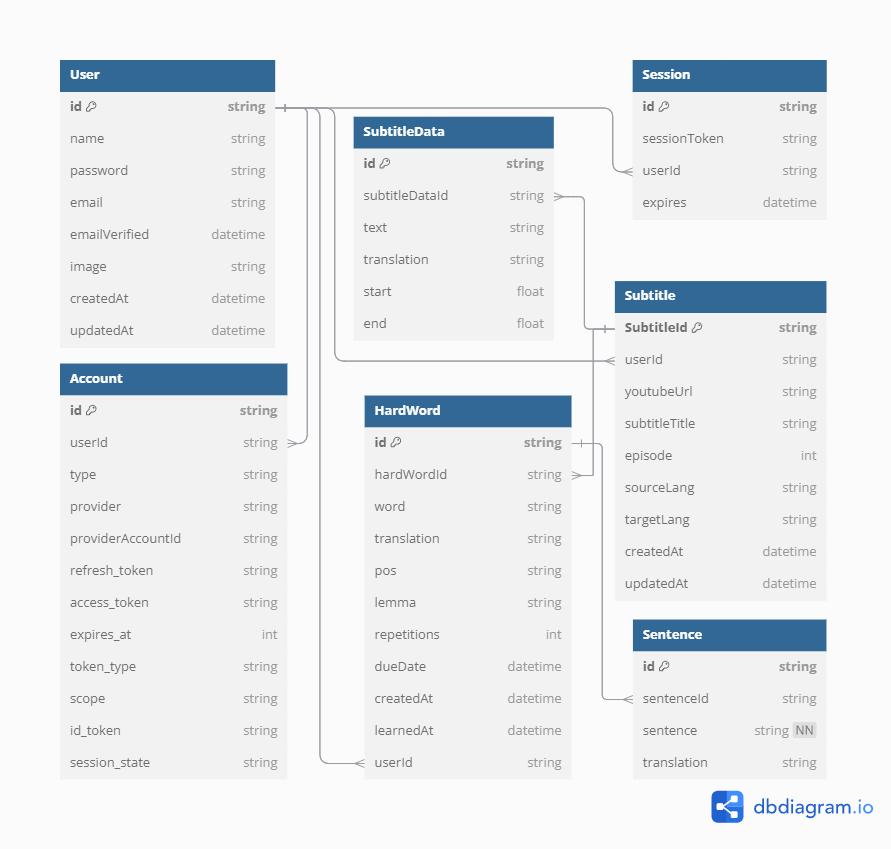
\includegraphics[width=1\textwidth]{IMAGE/DatabaseDiagram.png}
    \caption{Diagram struktury bazy danych}
    \label{fig:StrukturaBazyDanych}
\end{figure}
\subsection{Metody zapobiegania redundancji danych}
W celu zapobiegania redundancji danych w aplikacji zastosowano kilka metod. Przede wszystkim, projekt bazy danych został starannie zaplanowany, aby zminimalizować duplikację danych. Wykorzystano normalizację danych, która polega na podziale danych na mniejsze, logicznie powiązane tabele lub kolekcje, co pozwala na uniknięcie powtarzania tych samych informacji w różnych miejscach.

Dodatkowo, w aplikacji zaimplementowano mechanizmy walidacji danych, które sprawdzają poprawność i spójność danych przed ich zapisaniem do bazy. Dzięki temu możliwe jest wykrycie i eliminacja ewentualnych duplikatów na etapie wprowadzania danych. Poza jednym duplikatem, którym jest kolekcja zdania "sentence" gdy użytkownik usunie napisy z kolekcji "subtitles" to wtedy w kolekcji "sentence" pozostanie zdanie, które w trakcie nauki z słowami pozostaną bezpiecznie w bazie.

Wykorzystano również indeksy unikalne, które zapewniają, że w danej kolekcji nie mogą istnieć dwa dokumenty z identycznymi wartościami w polach, które powinny być unikalne. Na przykład, w kolekcji użytkowników zastosowano indeks unikalny na polu adresu e-mail, co zapobiega rejestracji dwóch użytkowników z tym samym adresem e-mail. W kolekcji słów zastosowano indeks unikalny na polu słowa "word", co zapobiega dodaniu dwóch  identycznych słów przez jednego użytkownika. To samo dotyczy kolekcji napisów, gdzie zastosowano indeks unikalny na polu tytułowym "subtitleTitle" w połączeniu z odcinkiem "episode" co nie pozwala przypadkowo dodać dwa takie same tytuły w połączeniu z odcinkiem.

Kolejną metodą zapobiegania redundancji jest stosowanie referencji między kolekcjami. Zamiast przechowywać duplikaty danych, dokumenty w jednej kolekcji mogą zawierać referencje do dokumentów w innych kolekcjach. Na przykład, dokumenty w kolekcji sesji użytkownika mogą zawierać referencje do dokumentów w kolekcji użytkowników, co pozwala na przechowywanie informacji o użytkownikach w jednym miejscu i uniknięcie redundancji.

Wszystkie te metody razem zapewniają, że dane w bazie są przechowywane w sposób efektywny i bez zbędnej redundancji, co przekłada się na lepszą wydajność i spójność danych.

\section{Interfejs użytkownika}
Interfejs użytkownika aplikacji składa się z kilku głównych widoków, które umożliwiają użytkownikom korzystanie z różnych funkcji. Wszystkie widoki zostały zaprojektowane z myślą o prostocie i intuicyjności, aby zapewnić użytkownikom łatwą nawigację i szybki dostęp do potrzebnych informacji. Poniżej przedstawiono najważniejsze elementy interfejsu użytkownika.


\subsection{Widok startowy}

\begin{figure}[H]
    \centering
    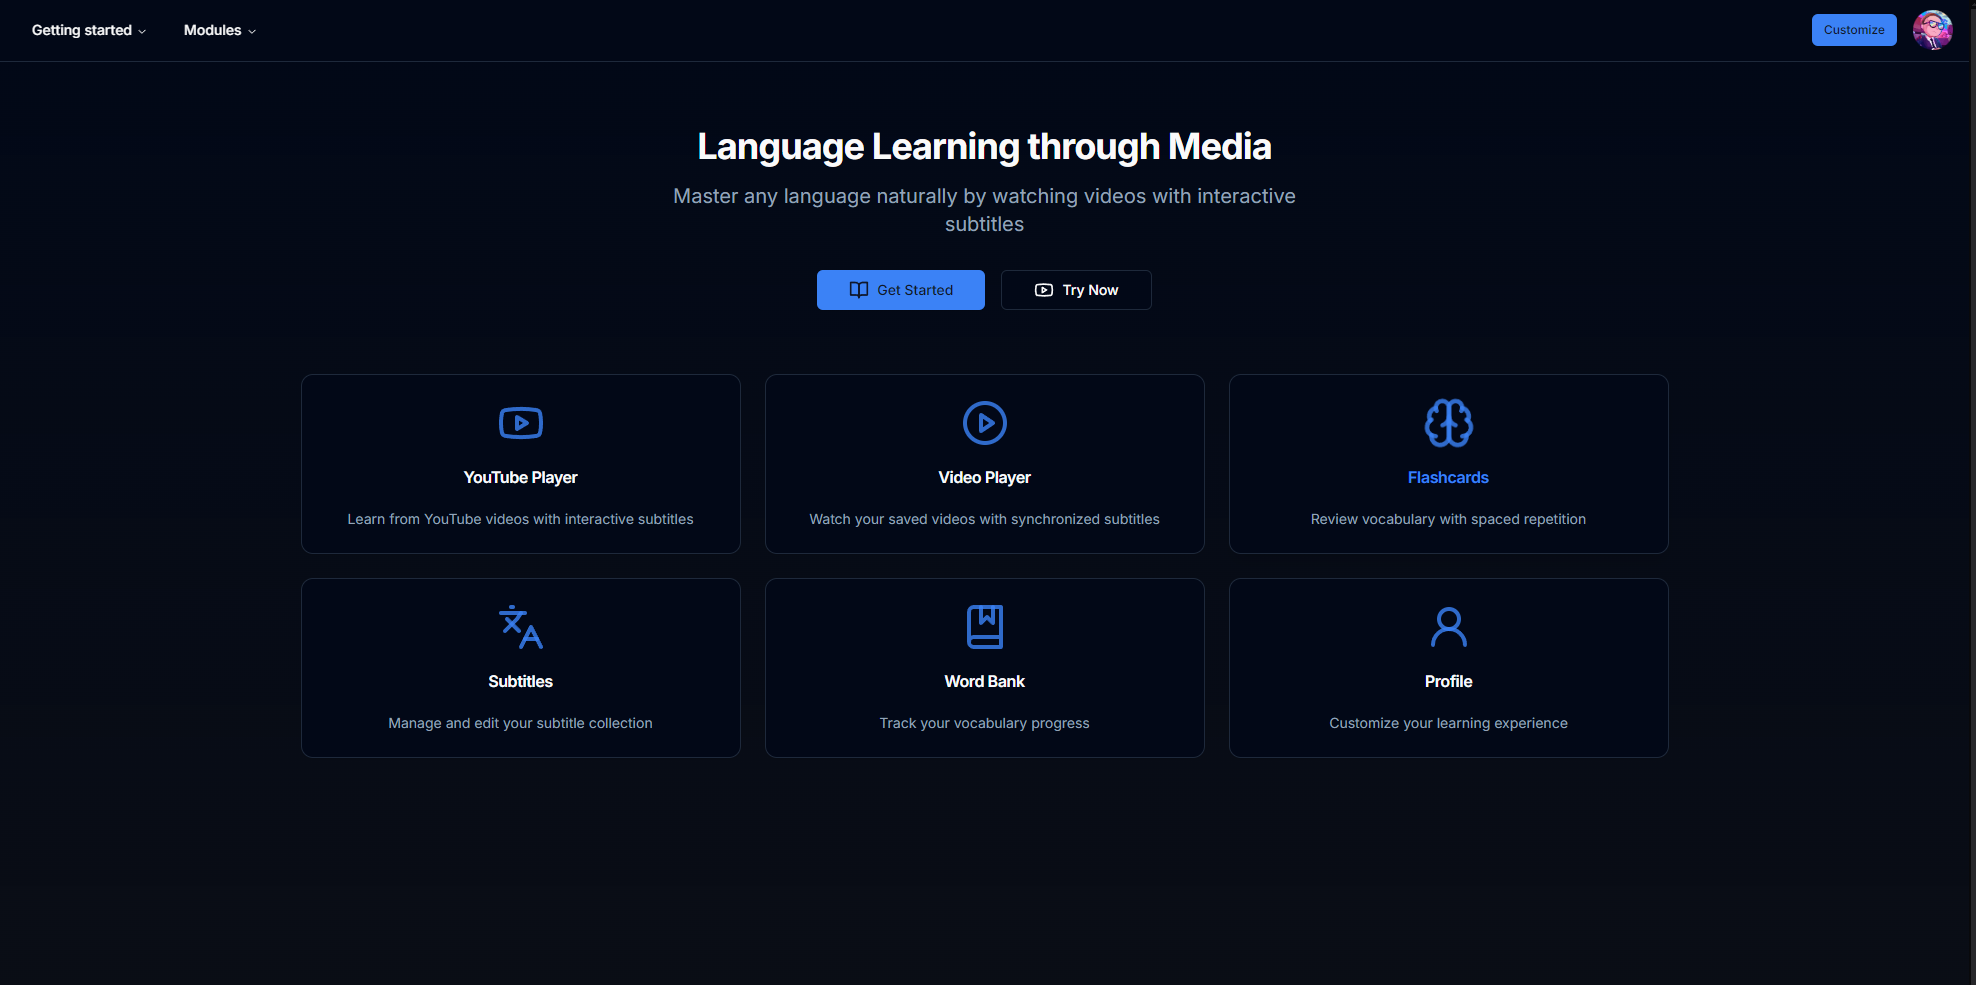
\includegraphics[width=1\textwidth]{IMAGE/HomePage.png}
    \caption{Strona główna aplikacji}
    \label{fig:Widok strony głównej aplikacji}
\end{figure}
Strona główna aplikacji zawiera przyciski kierujace do innych sekcji aplikacji, takich jak nauka, słownik, statystyki, profil użytkownika, ustawienia, itp. Użytkownicy mogą również przeglądać najnowsze filmy i seriale dostępne w aplikacji oraz korzystać z wyszukiwarki, aby znaleźć interesujące ich treści.

\subsection{Strona Nauki}

\begin{figure}[H]
    \centering
    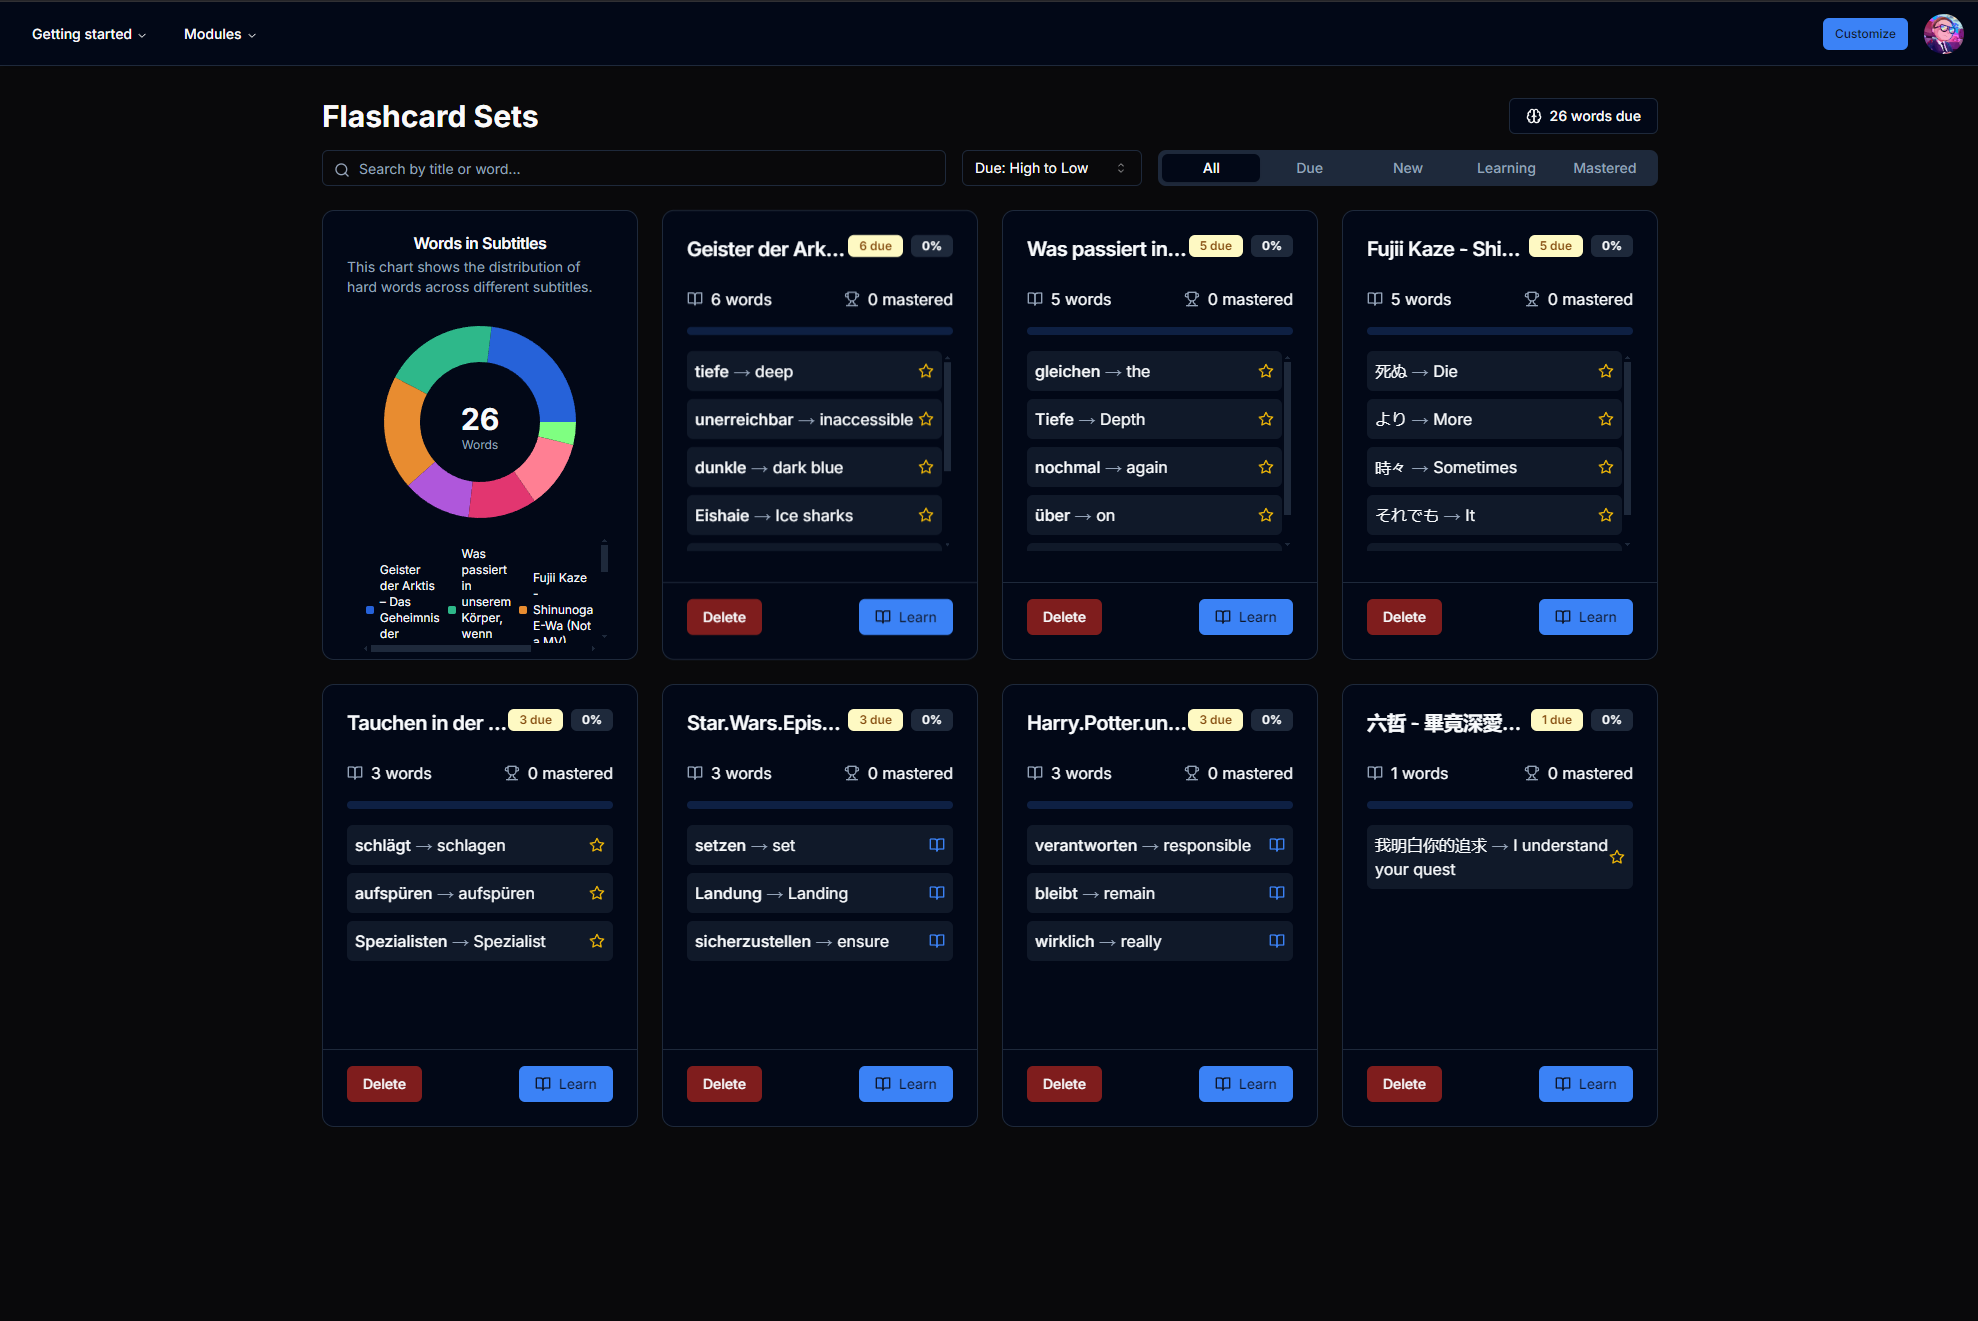
\includegraphics[width=1\textwidth]{IMAGE/FlashCards.png}
    \caption{Widok strony głównej fiszek}
    \label{fig:Strona głowna fiszek}
\end{figure}
\begin{figure}[H]
    \centering
    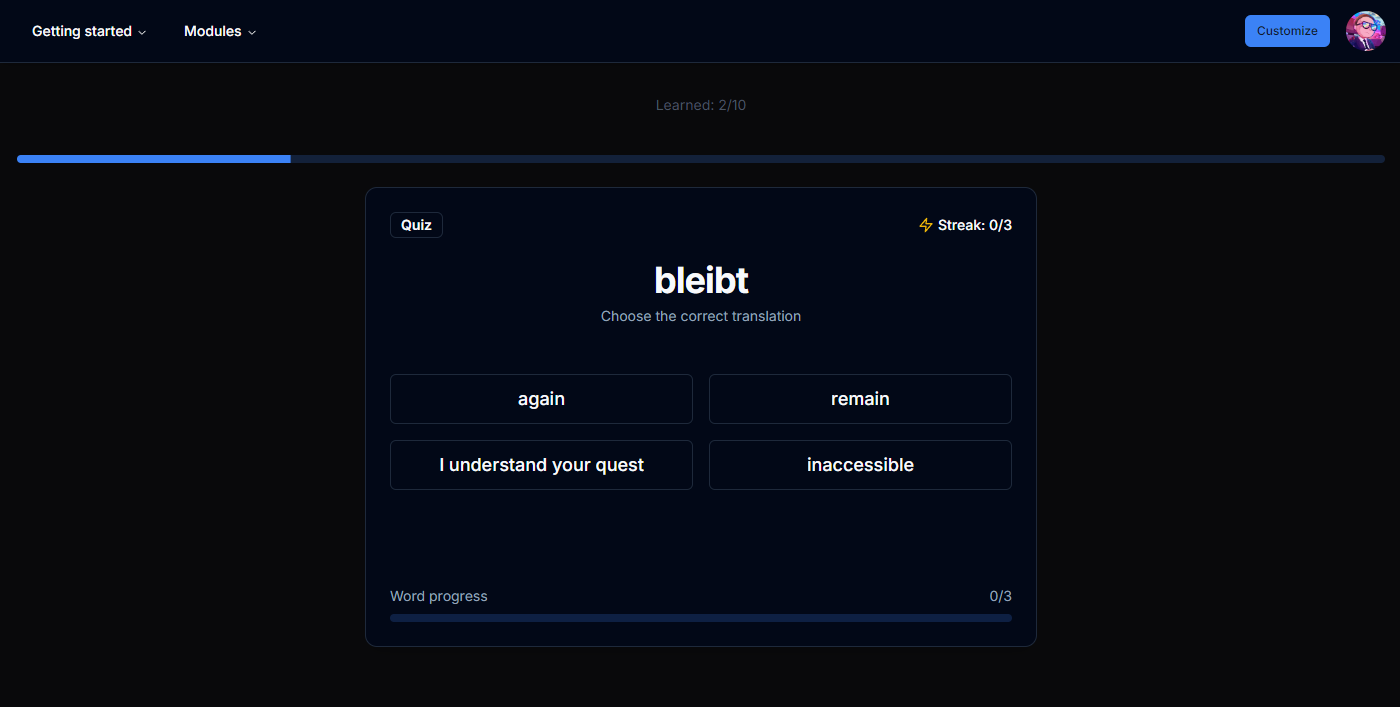
\includegraphics[width=1\textwidth]{IMAGE/Quiz.png}
    \caption{Widok quizu}
    \label{fig:Nauka z quizem}
\end{figure}
Strona Nauki to główne miejsce, w którym użytkownicy mogą korzystać z panelu nauki fiszek lub quizu. Panel fiszek zawiera informacje na temat stanu słów które są nowe, w trakcie nauki, lub skończone. Strona quizu umożliwia użytkownikom nauke poprzez quizy, w których użytkownicy muszą wybrać poprawne tłumaczenie słowa. Użytkownicy muszą poprawnie odpowiedzieć 3 razy z rzędu by słowo zostało uznane za nauczone i przeszło do kolejnego etapu którym jest powtórka po upływie odpowiedniego czasu.

\subsection{Strona Napisów}

\begin{figure}[H]
    \centering
    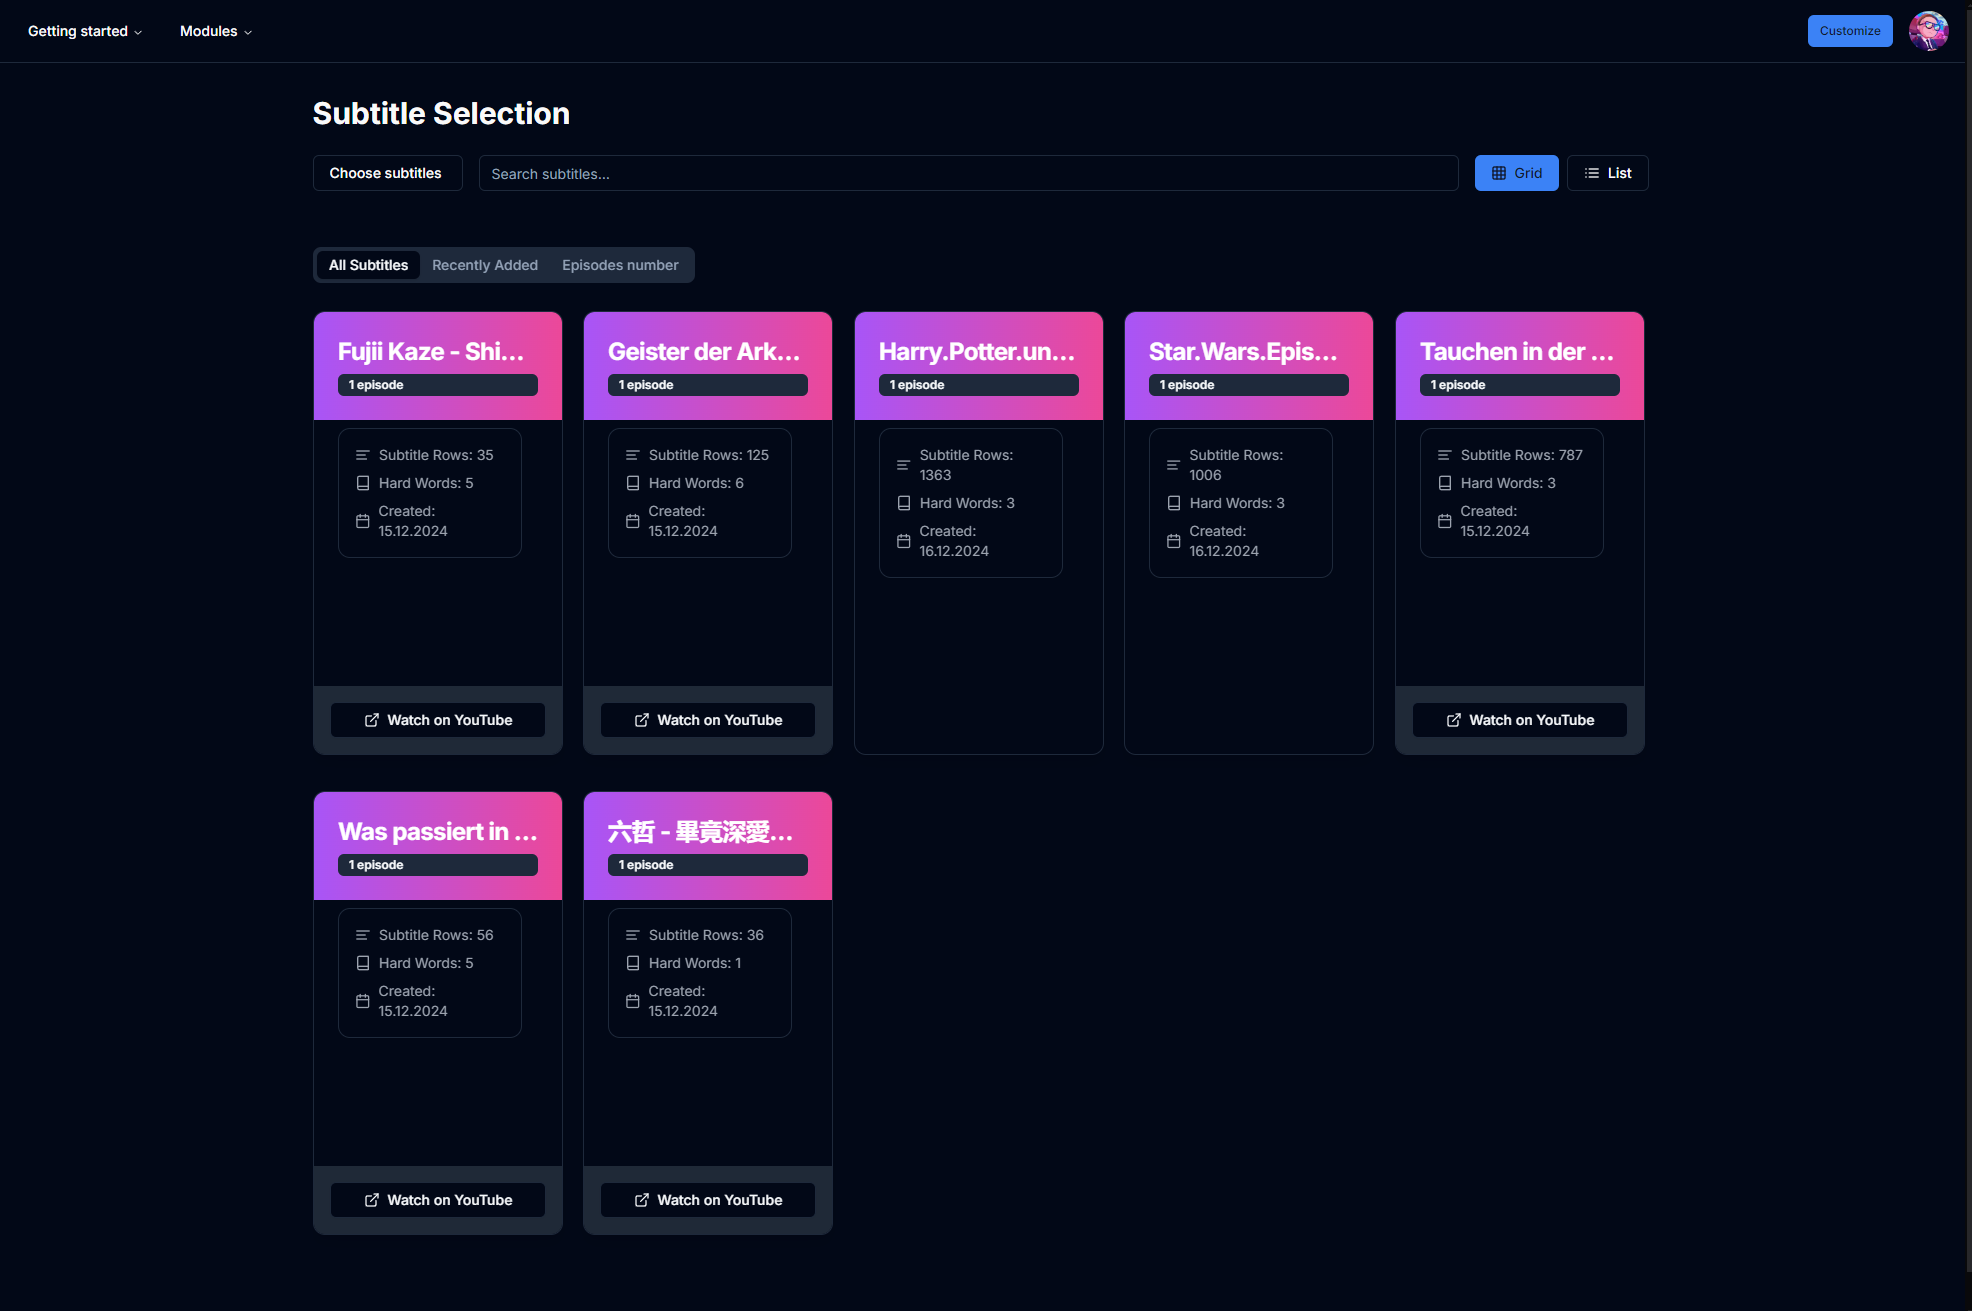
\includegraphics[width=1\textwidth]{IMAGE/Subtitles.png}
    \caption{Widok strony napisów}
    \label{fig:Strona napisów}
\end{figure}
Strona główna umożliwia wyszukiwanie zapisanych napisów, dostępne jest wyszukiwanie po tytule. Użytkownicy mogą również sortować napisy według daty dodania oraz liczby odcinków. Panel daje również możliwość zmiany wyświetlania między siatką a listą domyślnie jest to siatka maksymalnie 5 elementów na wiersz w zależności od miejsca na ekranie.

\begin{figure}[H]
    \centering
    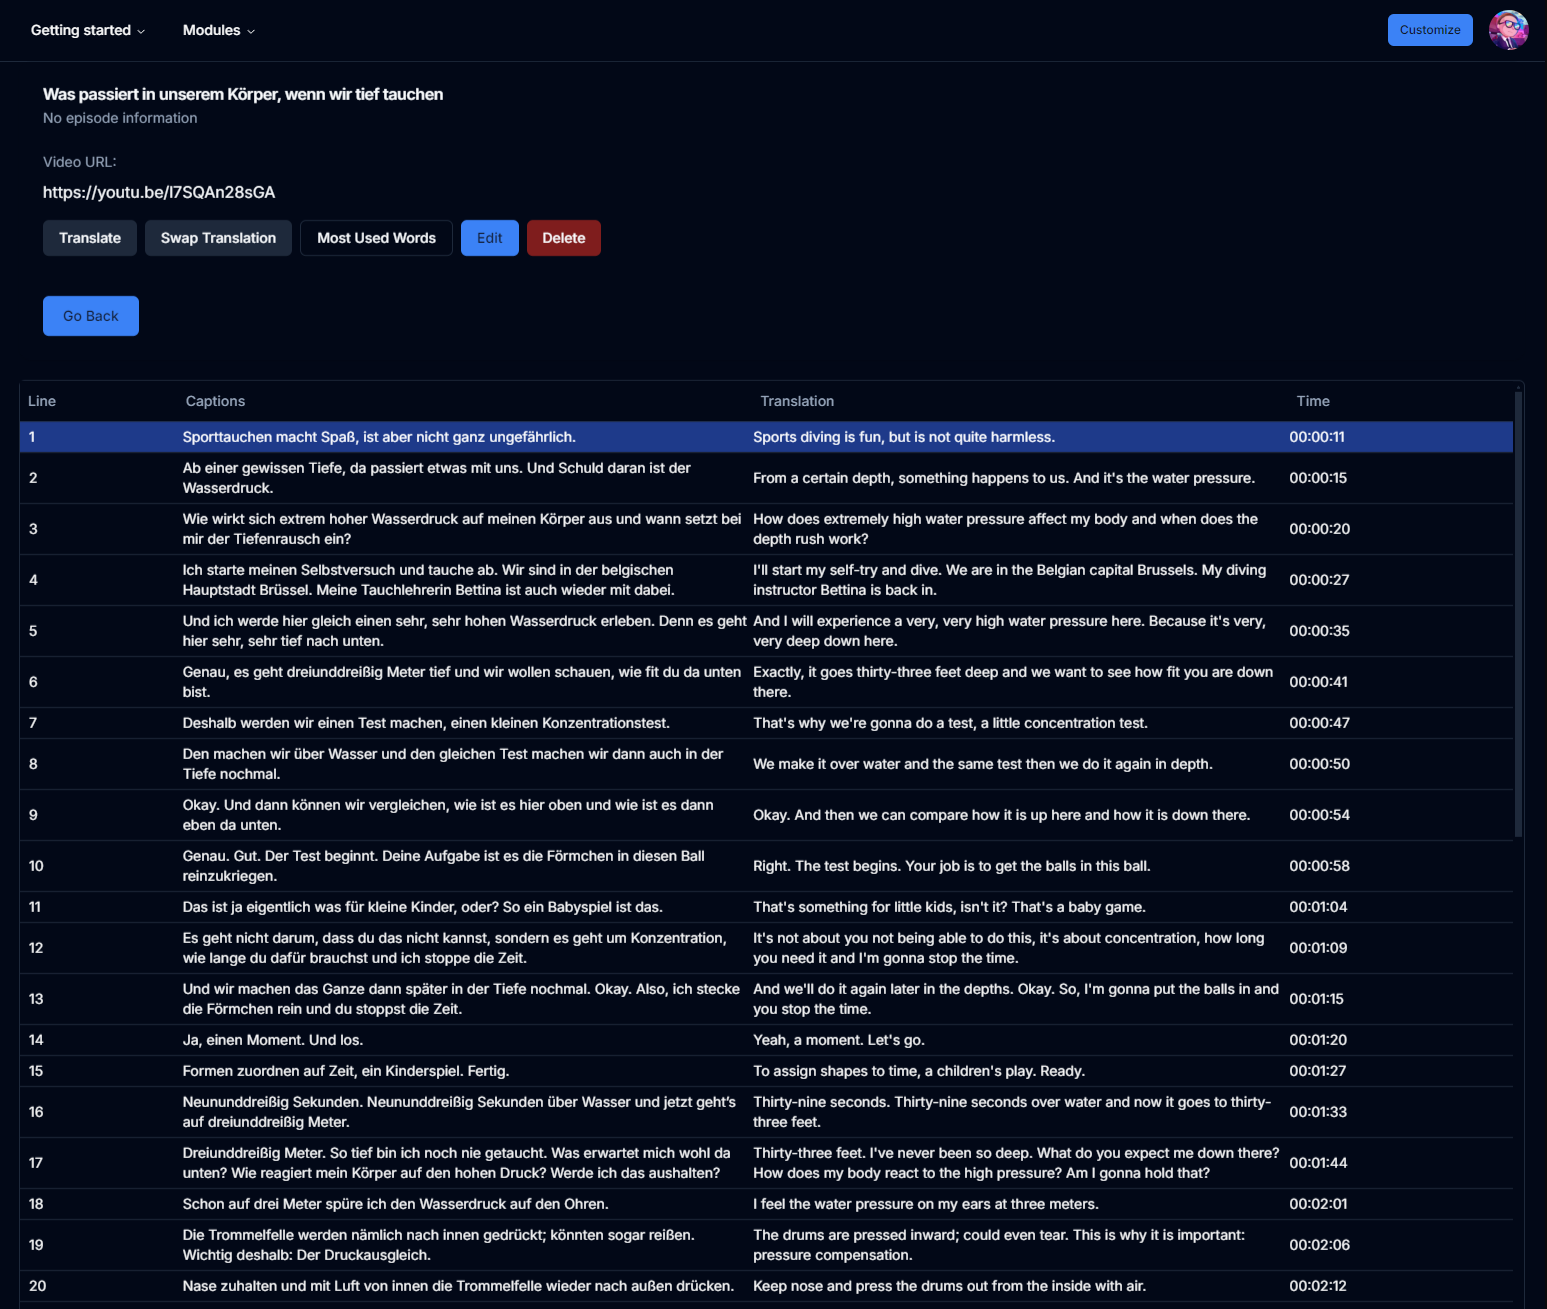
\includegraphics[width=1\textwidth]{IMAGE/SubtitlesSelected.png}
    \caption{Widok edycji napisów}
    \label{fig:Edycja napisów}
\end{figure}
Strona Napisów umożliwia użytkownikom przeglądanie i edycję napisów w bazie danych. Użytkownicy mogą edytować istniejące napisy, usuwać napisy, a także przeglądać listę wszystkich napisów w bazie z pomocą sortowania i wyszukiwania.

\subsection{Strona Słownika}

\begin{figure}[H]
    \centering
    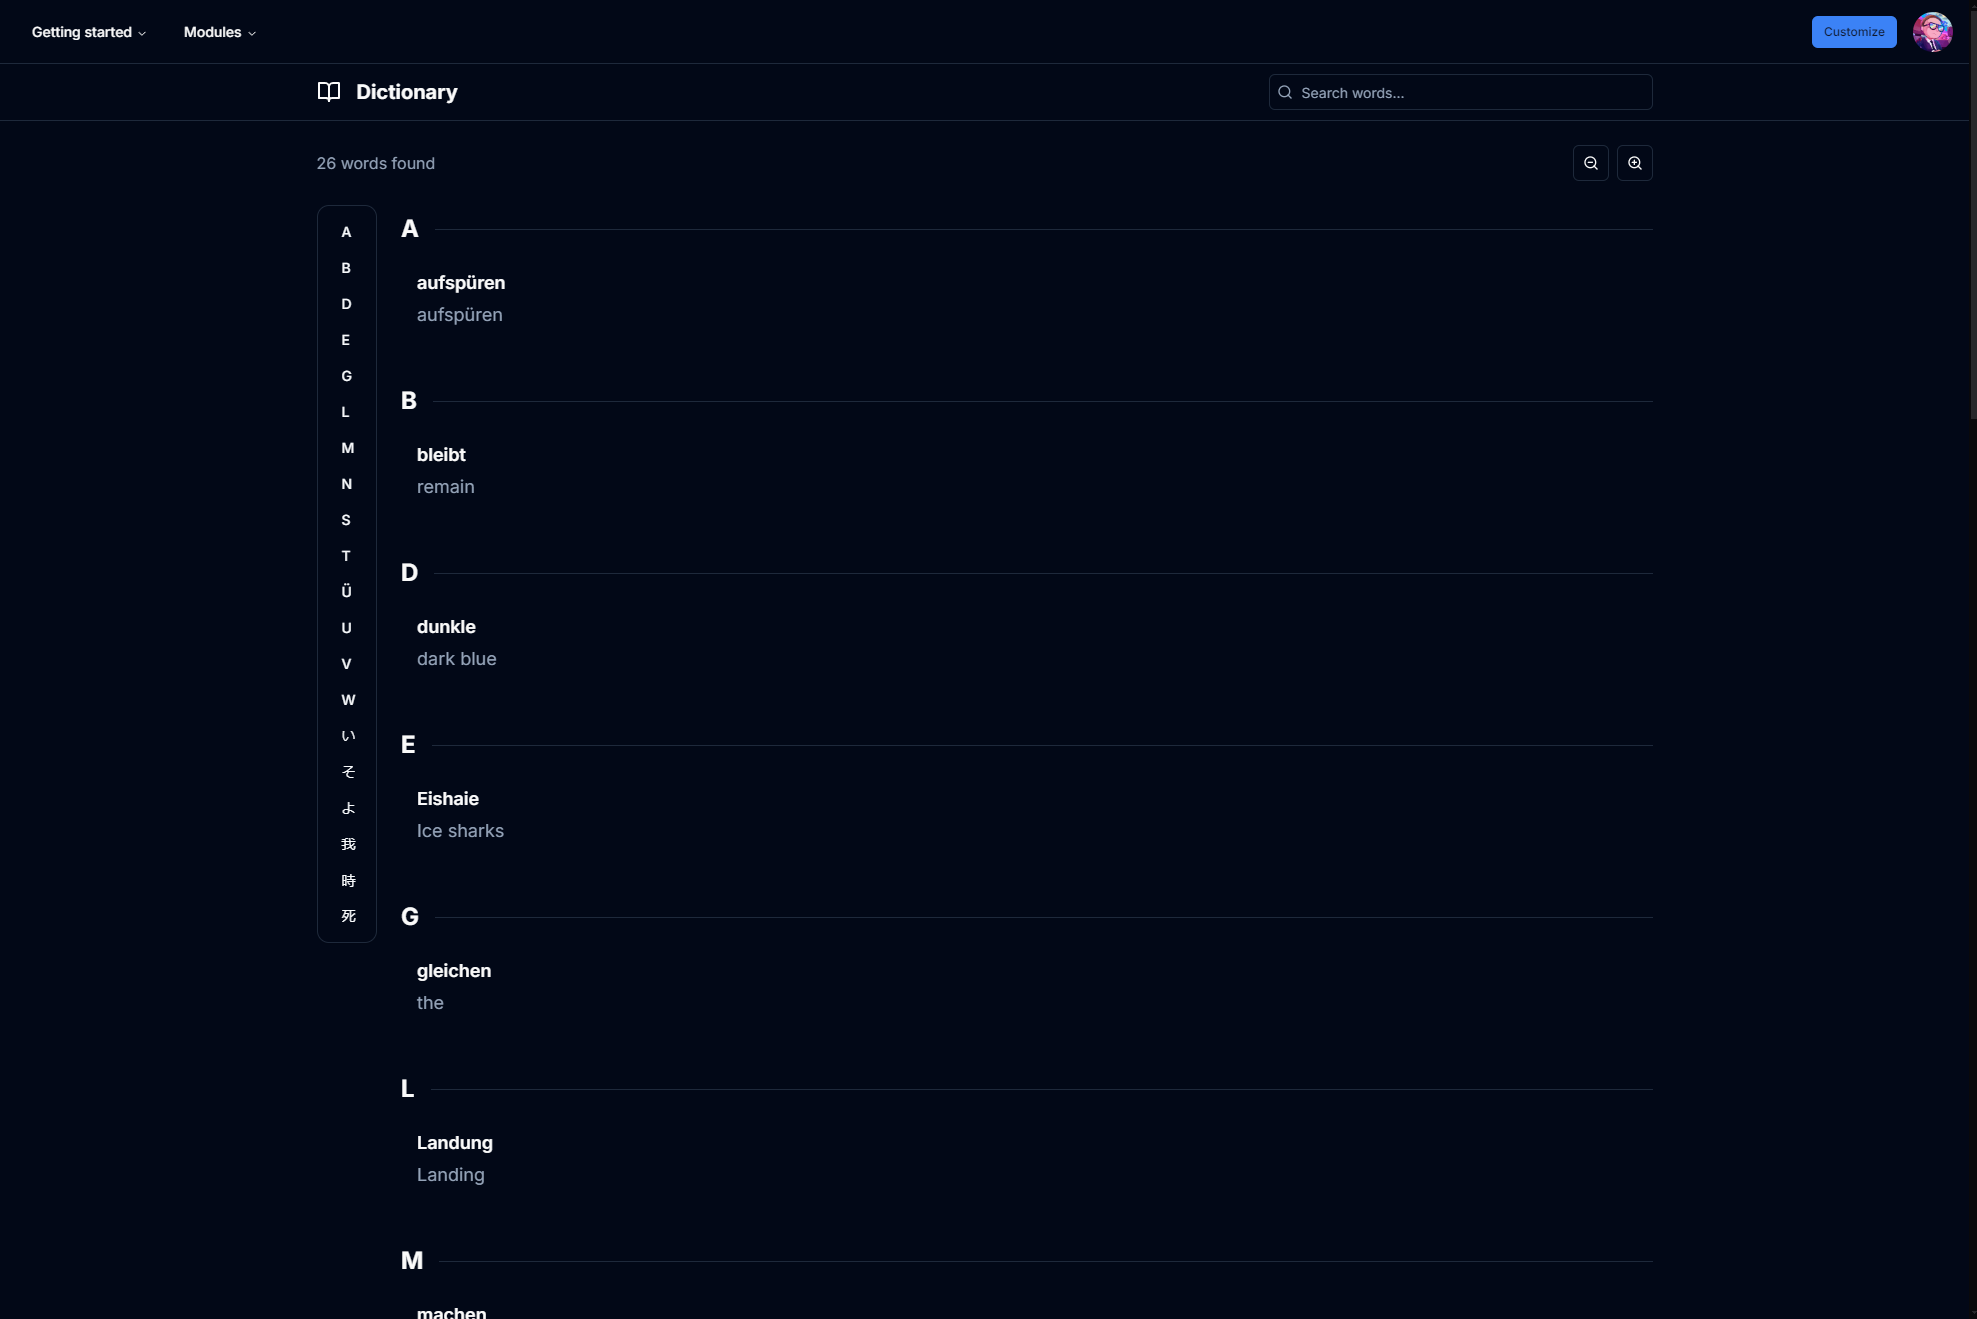
\includegraphics[width=1\textwidth]{IMAGE/WordBank.png}
    \caption{Widok słownika}
    \label{fig:Słownik słów}
\end{figure}
Strona Słownika umożliwia użytkownikom przeglądanie i edycję słów w bazie danych. Użytkownicy mogą  edytować istniejące słowa, usuwać słowa, a także przeglądać listę wszystkich słów w bazie z pomocą sortowania i wyszukiwania. Panel obsługuje również chińskie znaki.
\subsection{Strona Statystyk}

\begin{figure}[H]
    \centering
    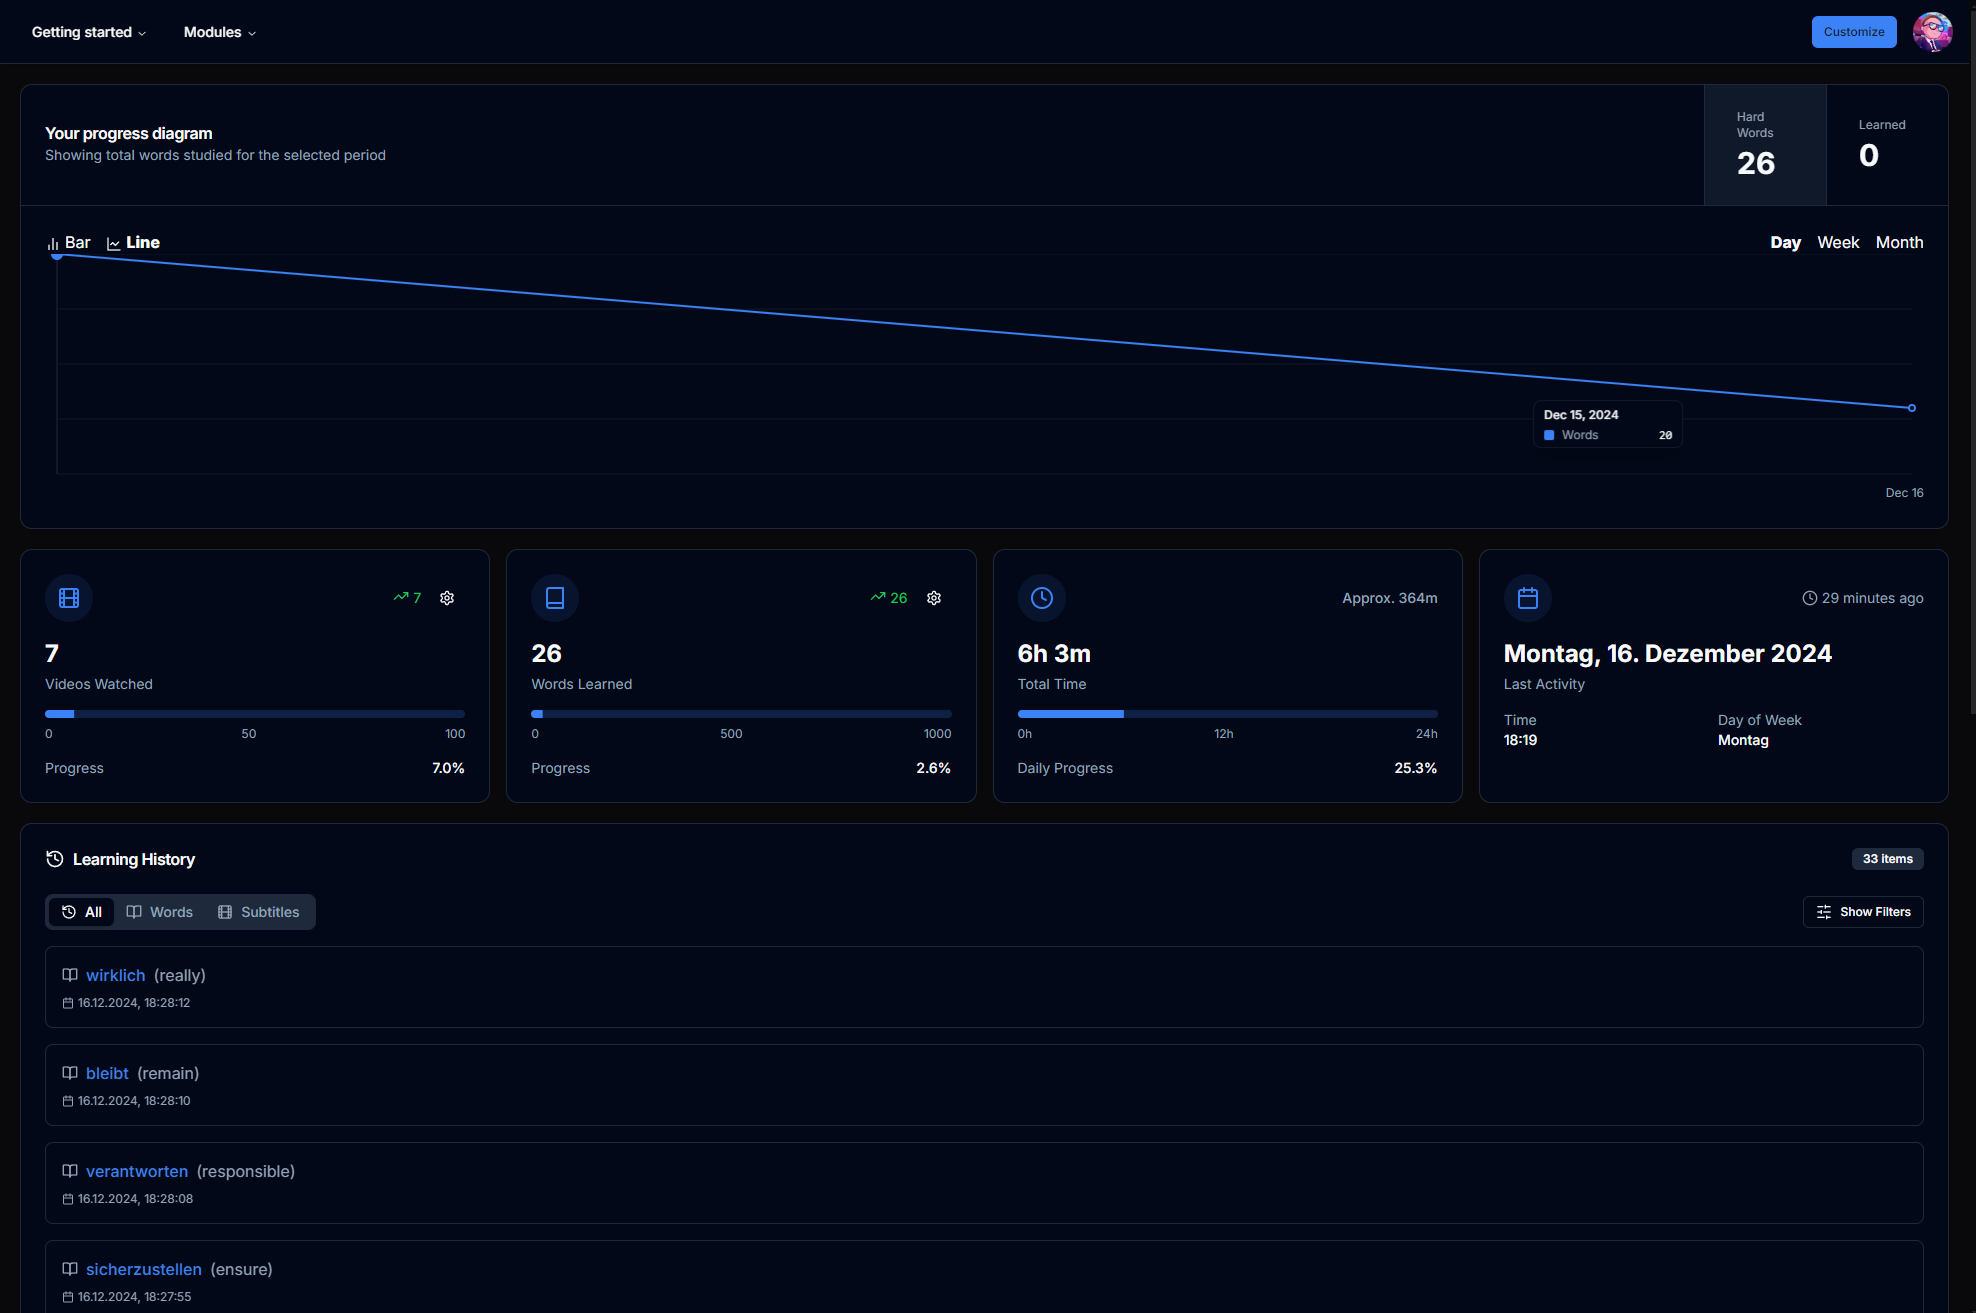
\includegraphics[width=1\textwidth]{IMAGE/Progress.png}
    \caption{Widok statystyk i postępów}
    \label{fig:Statystyki postępów}
\end{figure}
Strona Statystyk zawiera wykresy i statystyki dotyczące postępów w nauce użytkowników. Użytkownicy mogą śledzić swoje postępy w nauce słówek. Panel zawiera również informacje na temat liczby nowych słówek, oraz słówek nauczonych już wraz z datami utworzenia słowa i ukończenia nauki.
\subsection{Strona logowania oraz rejestracji}

\begin{figure}[H]
    \centering
    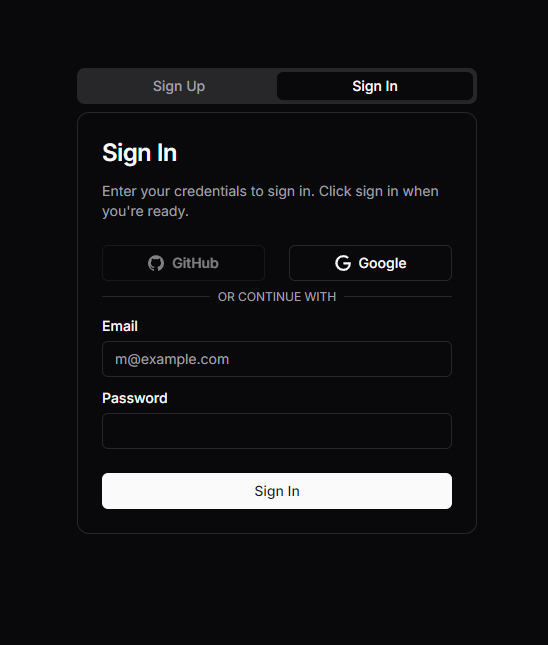
\includegraphics[width=1\textwidth]{IMAGE/LoginPage.png}
    \caption{Widok logowania i rejestracji}
    \label{fig:Logowanie i rejestracja}
\end{figure}
Strona logowania i rejestracji umożliwia użytkownikom zalogowanie się do aplikacji lub utworzenie nowego konta. Użytkownicy mogą wprowadzić swoje dane logowania, takie jak adres e-mail i hasło, aby uzyskać dostęp do aplikacji. Panel obsługuje również logowanie za pomocą konta Google, Logowanie za pomocą GitHub będzie dodane również pózniej.
\subsection{Strona oglądania filmów}


\begin{figure}[H]
    \centering
    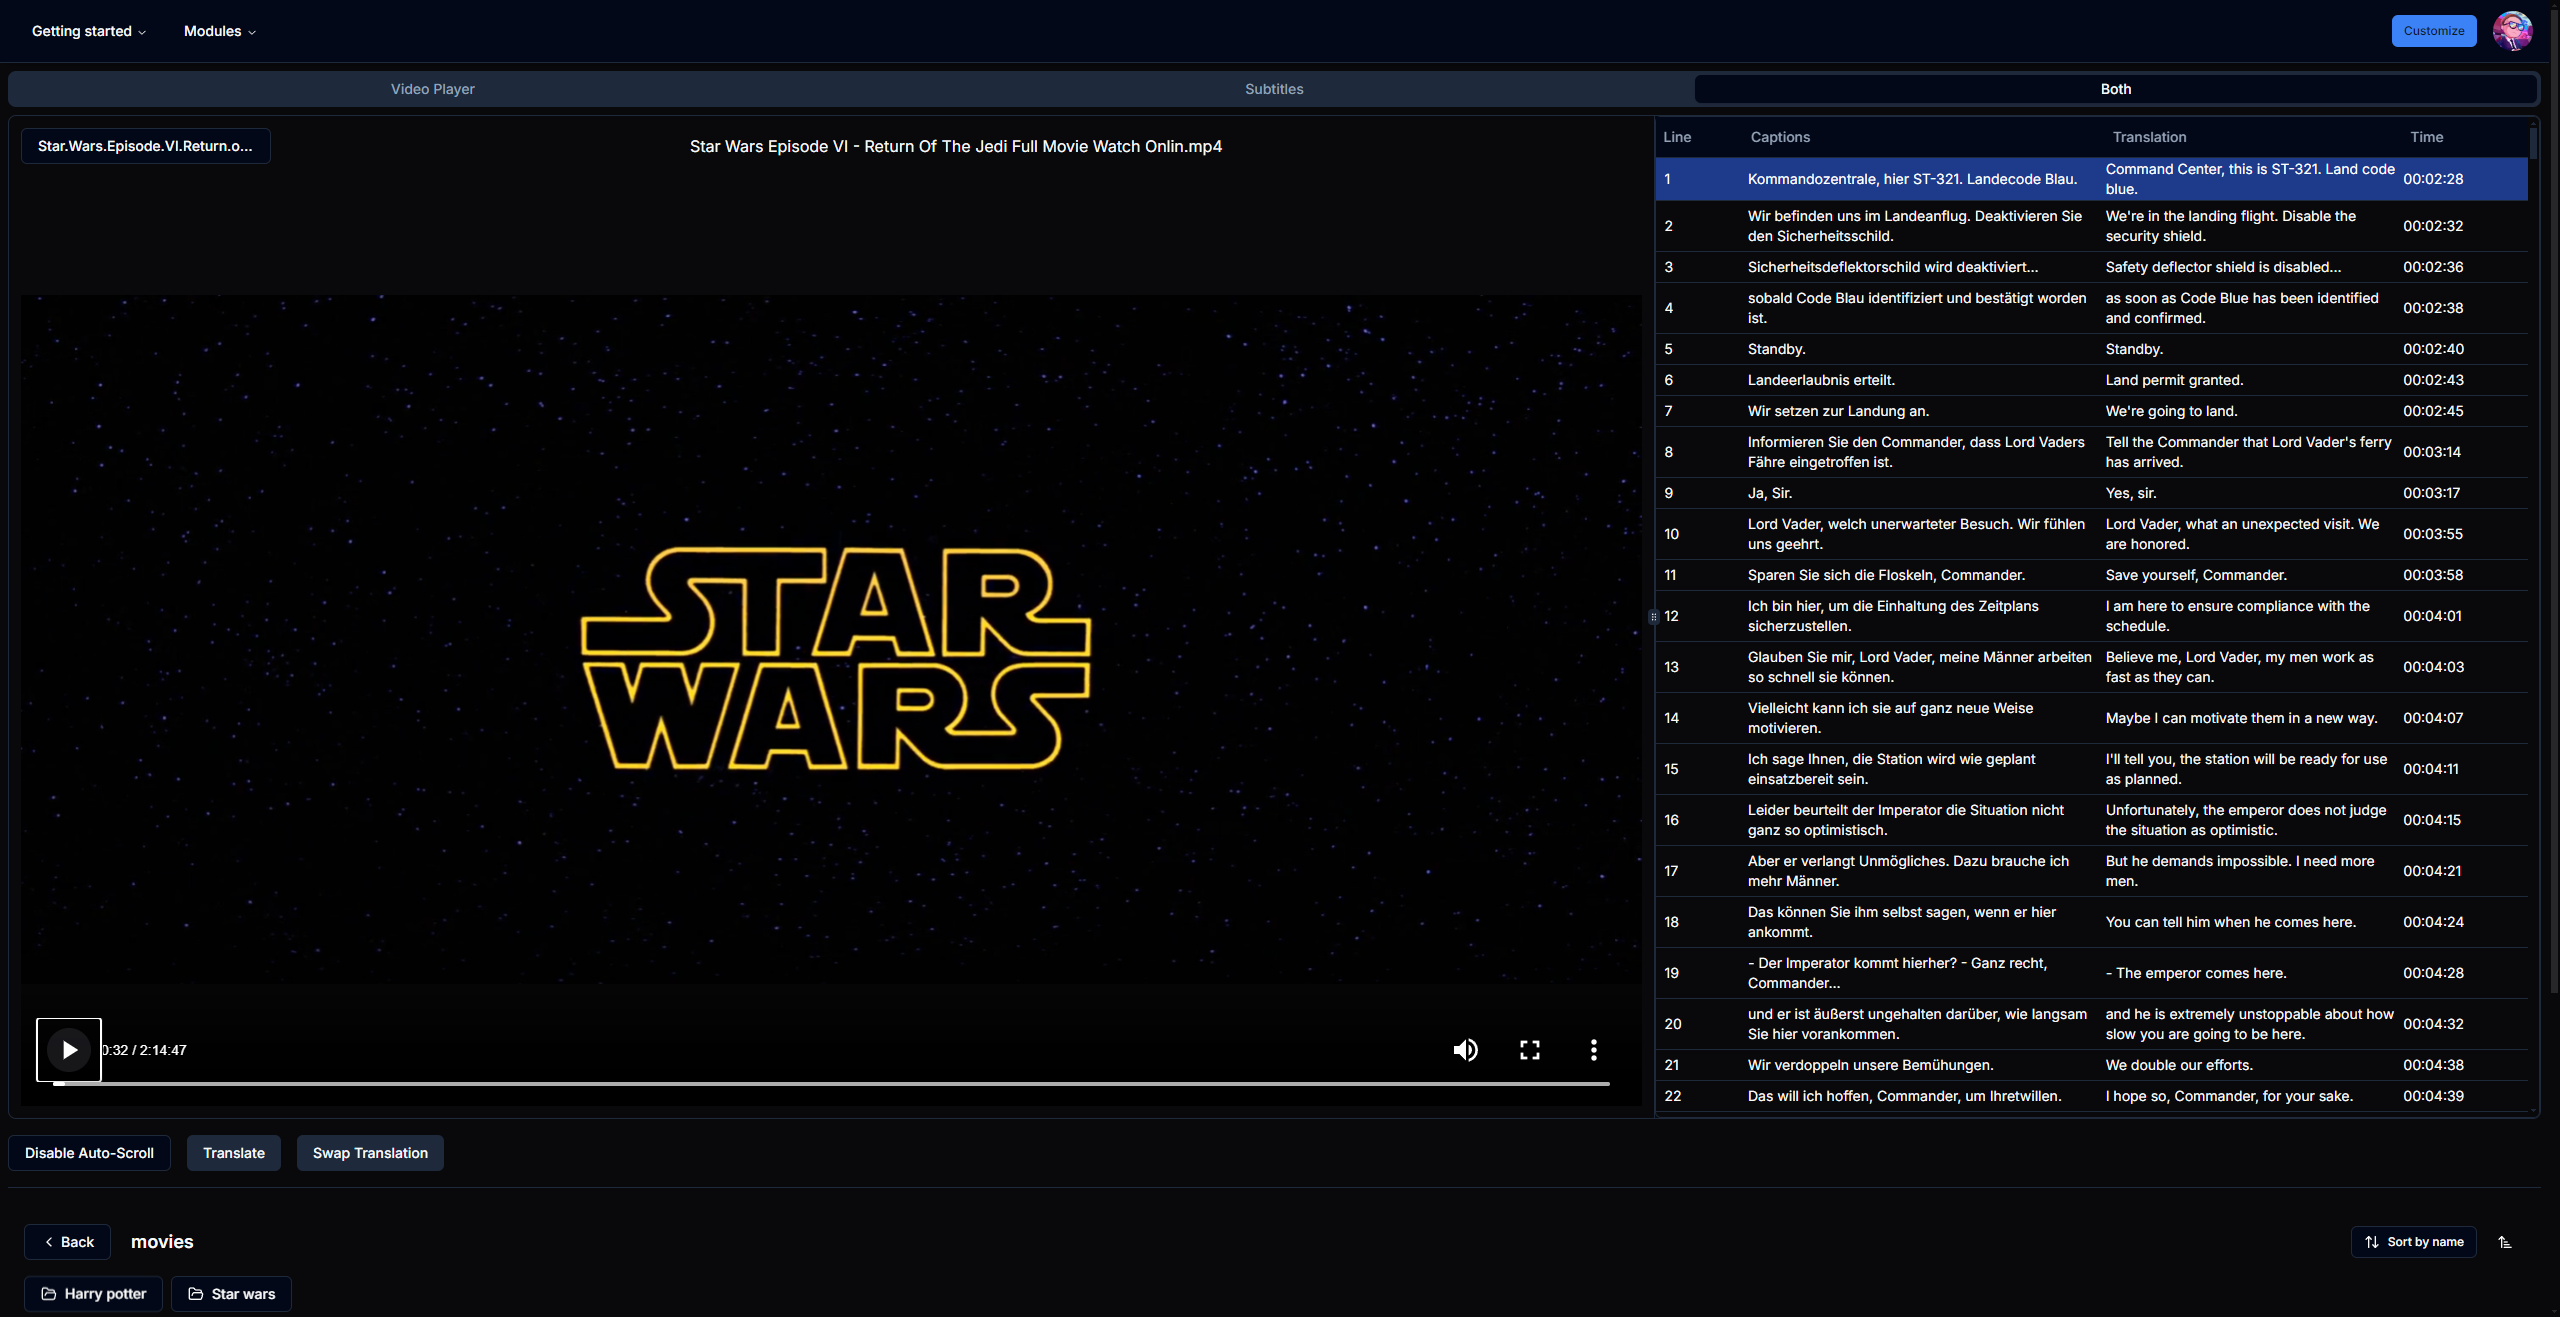
\includegraphics[width=1\textwidth]{IMAGE/videoPlayer.png}
    \caption{Widok oglądania filmów}
    \label{fig:oglądanie filmów}
\end{figure}

Strona oglądania filmów umożliwia użytkownikom przeglądanie i odtwarzanie filmów i seriali z listy zapisanych napisów i wybrania odpowiedniego filmu z dysku. Użytkownicy mogą zamienić szybko jezyk orginalny z przetłumaczonym lub włączyć śledzenie aktualnego wiersza napisów względem filmu "auto-scroll", a następnie rozpocząć oglądanie. Panel obsługuje również przewijanie filmu, zmianę języka napisów, oraz dodawanie słów do bazy w celu pózniejszej nauki. Użytkownik ma do wyboru albo filmy z rozszerzeniem mp4 albo mkv a napisy w formacie srt lub ass.





\chapter{Opracowanie szablonu pracy dyplomowej}
\section{Wprowadzenie}
W tej sekcji przedstawiono szczegółowy opis implementacji projektu, w tym wybór technologii, narzędzi programistycznych oraz środowiska, w którym został zrealizowany. Omówione zostaną również kluczowe aspekty techniczne, takie jak struktura bazy danych, architektura backendu i frontendu, a także proces testowania i napotkane problemy implementacyjne. Celem tej sekcji jest dostarczenie pełnego obrazu technicznego projektu oraz uzasadnienie wyboru poszczególnych rozwiązań technologicznych.


\section{Środowisko i narzędzia programistyczne}

\subsection{Środowisko programistyczne}
Do implementacji projektu wykorzystano następujące narzędzia i środowiska programistyczne:
\begin{itemize}
    \item \textbf{Visual Studio Code:} Środowisko programistyczne do tworzenia aplikacji internetowych w JavaScript i Python.
    \item \textbf{Git:} System kontroli wersji do zarządzania kodem źródłowym projektu.
    \item \textbf{MongoDB Atlas:} Usługa do hostowania bazy danych MongoDB w chmurze.
    \item \textbf{Flask:} Środowisko do tworzenia aplikacji webowych w Pythonie.
    \item \textbf{TypeScript:} Język programowania, który kompiluje się do JavaScriptu i dodaje typy danych w kodzie.

\end{itemize}
\subsection{Wybór technologii}
W trakcie realizacji projektu wykorzystano następujące technologie:
\begin{itemize}
    \item \textbf{Next.js:} Framework do tworzenia aplikacji internetowych w React, który oferuje wiele wbudowanych funkcji, takich jak routing, server-side rendering czy generowanie statyczne \cite{nextjs}.
    \item \textbf{Python:} Język programowania, który wykorzystałem do implementacji algorytmów przetwarzania języka naturalnego (NLP).
    \item \textbf{React Virtuoso:} Biblioteka do wirtualizacji list w aplikacjach internetowych.
    \item \textbf{Node.js:} Środowisko uruchomieniowe JavaScript, które pozwala na tworzenie aplikacji serwerowych.
    \item \textbf{MongoDB:} Baza danych NoSQL, która umożliwia przechowywanie danych w formacie JSON.
    \item \textbf{React.js:} Biblioteka do tworzenia interfejsów użytkownika w aplikacjach internetowych.
    \item \textbf{Shadcn:} Bibloteka gotowych komponentów do budowy interfejsu użytkownika w React.
    \item \textbf{Redux:} Biblioteka do zarządzania stanem aplikacji w React.
    \item \textbf{Prisma:} ORM do zarządzania bazą danych w Node.js.
    \item \textbf{Axios:} Biblioteka do wykonywania zapytań HTTP w JavaScript.
    \item \textbf{Tailwind CSS:} Narzędzie do tworzenia stylów CSS za pomocą gotowych klas, umożliwiające szybkie projektowanie responsywnych interfejsów.
\end{itemize}

\subsection{Opis technologii}
\subsubsection{Next.js}
Next.js to framework do tworzenia aplikacji internetowych w React, który oferuje wiele wbudowanych funkcji, takich jak routing, server-side rendering czy generowanie statyczne. Dzięki temu można tworzyć wydajne i skalowalne aplikacje internetowe, które są przyjazne dla SEO i łatwe w utrzymaniu. Next.js oferuje również wiele gotowych rozwiązań, takich jak automatyczne generowanie ścieżek, obsługa dynamicznych routów czy optymalizacja obrazów \cite{nextjs}. Dzięki temu można skupić się na tworzeniu funkcjonalności, zamiast martwić się o konfigurację i optymalizację aplikacji.
Kolejną istotną zaletą Next.js jest intuicyjny i wydajny system routingu oparty na strukturze plików. Ułatwia to organizację aplikacji i nawigację po niej, co jest kluczowe dla zachowania przejrzystości i spójności struktury. Next.js oferuje również uproszczone pobieranie danych oraz wsparcie dla różnych metod stylizacji, takich jak moduły CSS i Tailwind CSS, co pozwala na tworzenie estetycznego i responsywnego interfejsu użytkownika szybciej i łatwiej. Dodatkowo, framework zapewnia wsparcie dla TypeScript, co umożliwia tworzenie bezpiecznego i stabilnego kodu przy użyciu typów które nam podkreślą jeśli będziemy próbowali błędnie używac naszych funkcji lub zmiennych. Wszystkie te cechy czynią Next.js idealnym wyborem do stworzenia nowoczesnej i wydajnej aplikacji językowej \cite{bui2023next}.

\subsubsection{Python}
Python to język programowania, który wykorzystałem do implementacji algorytmów przetwarzania języka naturalnego (NLP). Python jest popularny w dziedzinie analizy danych i uczenia maszynowego, dzięki czemu można znaleźć wiele gotowych bibliotek i narzędzi do przetwarzania tekstu. W moim projekcie wykorzystałem biblioteki takie jak NLTK, spaCy czy TextBlob do lematyzacji, oznaczania części mowy i analizy sentymentu tekstu.

\subsubsection{React Virtuoso}
React Virtuoso to biblioteka do wirtualizacji list w aplikacjach internetowych. Umożliwia renderowanie długich list danych w sposób efektywny i wydajny, co przyczynia się do poprawy wydajności i płynności interfejsu użytkownika. Dzięki React Virtuoso można renderować tylko widoczne elementy i kilka dodatkowych poza obszarem.

\subsubsection{Node.js}
Node.js to środowisko uruchomieniowe JavaScript, które pozwala na tworzenie aplikacji serwerowych. Dzięki Node.js można pisać zarówno frontend, jak i backend w jednym języku programowania, co ułatwia rozwój i utrzymanie aplikacji. Node.js oferuje również wiele gotowych modułów i bibliotek, które ułatwiają tworzenie aplikacji internetowych, takich jak Express.js, Socket.io czy Mongoose \cite{bugl2024modern}.

\subsubsection{MongoDB}
Wybór bazy danych do aplikacji webowej ma ogromne znaczenie dla jej wydajności i skalowalności. W tym projekcie zdecydowano się na MongoDB Atlas, która jest objektową bazą danych typu NoSQL. MongoDB charakteryzuje się elastyczną strukturą danych, co pozwala na szybkie i efektywne przechowywanie oraz zarządzanie różnorodnymi danymi w formacie JSON. W projekcie baza danych została wykorzystana do przechowywania danych o użytkownikach, słowach do nauki, napisach oraz postępach w nauce.

\subsubsection{React.js}
React.js to biblioteka do tworzenia interfejsów użytkownika w aplikacjach internetowych. React.js oferuje wiele funkcji i narzędzi, które ułatwiają tworzenie interaktywnych i responsywnych interfejsów. Dzięki React.js można tworzyć komponenty UI, zarządzać stanem aplikacji i reagować na interakcje użytkownika w sposób efektywny i wydajny \cite{dinku2022react}.

\subsubsection{Shadcn}
Shadcn to kolekcja komponentów, które można kopiować i wklejać do swoich aplikacji. Nie jest to biblioteka komponentów, którą można zainstalować jako zależność. Shadcn nie jest dostępny ani dystrybuowany przez npm (node package manager). Użytkownik wybiera potrzebne komponenty, kopiuje i wkleja kod do swojego projektu, a następnie dostosowuje go do swoich potrzeb. Kod jest własnością użytkownika. Shadcn może służyć jako odniesienie do budowy własnych bibliotek komponentów. do rozbudowy interfejsu użytkownika w React. Shadcn oferuje wiele gotowych rozwiązań, takich jak przyciski, formularze, tabele czy karty, które można łatwo dostosować do własnych potrzeb. Dzięki Shadcn można tworzyć interfejsy użytkownika w sposób szybki i efektywny, co przyczynia się do skrócenia czasu potrzebnego na rozwój aplikacji.







% \section{Baza danych}
% Baza danych w projekcie została zaimplementowana przy użyciu MongoDB Atlas, która jest objektową bazą danych typu NoSQL. MongoDB charakteryzuje się elastyczną strukturą danych, co pozwala na szybkie i efektywne przechowywanie oraz zarządzanie różnorodnymi danymi w formacie JSON. W projekcie baza danych została wykorzystana do przechowywania danych o użytkownikach, słowach do nauki, napisach oraz postępach w nauce.

% Jedną z kluczowych zalet MongoDB jest jej skalowalność. Baza ta umożliwia łatwe skalowanie poziome, co oznacza, że możemy dodawać nowe serwery do naszego klastra bazodanowego w miarę wzrostu ilości danych i liczby użytkowników. Jest to szczególnie ważne dla aplikacji edukacyjnych, które mogą szybko rosnąć w popularność i wymagać zwiększonej mocy obliczeniowej. Dzięki temu, nasza aplikacja będzie mogła obsługiwać rosnącą liczbę użytkowników bez utraty wydajności. Dodatkowo, MongoDB Atlas oferuje wsparcie dla replikacji danych, co zwiększa niezawodność i dostępność systemu. Funkcja replikacji zapewnia, że dane są automatycznie kopiowane na wiele serwerów, co chroni przed utratą danych i zapewnia ciągłość działania aplikacji. Dzięki tym funkcjom MongoDB Atlas jest idealnym wyborem dla naszej aplikacji, zapewniając jej wydajność, skalowalność i elastyczność w zarządzaniu danymi.


% \subsection{Obsługa logowania Google}
% Obsługa logowania Google w aplikacji została zaimplementowana przy użyciu NextAuth.js w wersji 5.0.0. NextAuth.js to biblioteka do uwierzytelniania użytkowników w aplikacjach internetowych, która oferuje wiele funkcji i narzędzi, które ułatwiają proces logowania i rejestracji użytkowników. Dzięki NextAuth.js można łatwo dodawać różne metody uwierzytelniania, takie jak logowanie za pomocą Google, Facebooka czy GitHuba, co pozwala na dostosowanie aplikacji do indywidualnych potrzeb użytkowników. W projekcie zdecydowano się na obsługę logowania Google, ponieważ jest to popularna metoda uwierzytelniania, która jest łatwa w użyciu i zapewnia wysoki poziom bezpieczeństwa. Dzięki logowaniu Google użytkownicy mogą szybko i wygodnie zalogować się do aplikacji za pomocą swojego konta Google, co ułatwia korzystanie z aplikacji i zwiększa jej atrakcyjność dla użytkowników.




\section{Backend}
Backend aplikacji został zrealizowany przy użyciu dwóch technologii: Next.js oraz Flask. Każda z tych technologii pełni inną rolę w architekturze aplikacji, co pozwala na wykorzystanie ich mocnych stron w Flask został wykonany moduł pełniący funkcje lemmatyzacji i pos taggingu ponieważ modele NLP są tam bardzo mocno rozwinięte. W Next.js zostały wykonane endpointy do komunikacji z bazą danych oraz do obsługi logiki biznesowej aplikacji. Dzięki temu możliwe jest oddzielenie części serwerowej od frontendowej, co pozwala wykorzystać zalety szybkiego serwowania stron statycznych. Poniżej przedstawiono architekturę backendu z wykorzystaniem Next.js i Flask. Dodatkowo został wykorzystany moduł LibretTranslate do tłumaczenia maszynowego w aplikacji.

\subsubsection{Next.js}
Next.js jest wykorzystywany do obsługi części serwerowej aplikacji, która jest odpowiedzialna za renderowanie stron po stronie serwera (server-side rendering) oraz generowanie statycznych stron (static site generation). Dzięki temu aplikacja jest szybka i przyjazna dla SEO. Next.js umożliwia również łatwe zarządzanie ścieżkami strony które są wyświetlane w pasku url przeglądarki. Głównym celem w projekcie jest obsługa żądań HTTP, komunikacja z bazą danych MongoDB oraz wykonywanie operacji związanych z komunikacją z modułami NLP w Flask jak i modułem LibretTranslate do tłumaczenia maszynowego w aplikacji. Next.js oferuje również wsparcie dla różnych metod autoryzacji i uwierzytelniania, co zapewnia bezpieczeństwo aplikacji jak i szybkość działania i implementacji.
\subsection{Struktura backendu w Next.js}
Struktura backendu w Next.js została podzielona na kilka głównych katalogów, z których każdy odpowiada za określoną część aplikacji. Wszystkie pliki związane z budową backendu znajdują się w katalogu \texttt{src/app/api}, który zawiera następujące podkatalogi:

\begin{itemize}
    \item \textbf{auth:} Obsługuje autoryzację i uwierzytelnianie użytkowników.
    \item \textbf{captions:} Zajmuje się pobieraniem napisów z youtube.
    \item \textbf{hardWords:} Zajmuje się zarządzaniem trudnymi słowami.
    \item \textbf{profile:} Obsługuje aktualizacje profilu użytkownika.
    \item \textbf{sentence:} Zajmuje się aktualizacjami zdań.
    \item \textbf{signup:} Obsługuje rejestrację nowych użytkowników.
    \item \textbf{subtitles:} Zajmuje się zarządzaniem napisami do filmów.
\end{itemize}

\subsection{Struktura backendu w Flask}
Flask jest wykorzystywany do tworzenia API oraz logiki biznesowej aplikacji. Flask to lekki framework webowy dla Pythona, który umożliwia szybkie tworzenie i rozwijanie aplikacji webowych. W projekcie Flask jest odpowiedzialny za przetwarzanie żądań HTTP, oraz wykonywanie operacji związanych z przetwarzaniem języka naturalnego (NLP).
użyte do tego zostały modele:

\begin{lstlisting}[language=Python, caption=kod do importowania modeli NLP]
    nlp_de = spacy.load('de_core_news_md')
    nlp_ja = spacy.load('ja_core_news_md')
    nlp_en = spacy.load('en_core_web_md')
    nlp_pl = spacy.load('pl_core_news_md')
    
\end{lstlisting}

zostały one użyte do przetwarzania języka naturalnego w aplikacji. Dzięki temu możliwe jest lemmatyzacja i pos tagging słów w różnych językach. Do projektu zostały wykorzystane modele językowe dla języków: niemieckiego, japońskiego, angielskiego i polskiego. Reszta języków nie jest obsługiwana w aplikacji, ale można dodać nowe modele językowe w przyszłości.

\begin{lstlisting}[language=Python, caption=kod do obsługi lemmatyzacji i pos taggingu]
    @app.post("/nlp")
    async def analyze_text(request: AnalyzeTextRequest):
        word = request.word
        sourceLang = request.sourceLang
        doc = None
    
        if not sourceLang:
            raise HTTPException(status_code=400, detail="Source language is required")
        if sourceLang == 'de':
            doc = nlp_de(word)
        elif sourceLang == 'ja':
            doc = nlp_ja(word)
        elif sourceLang == 'en':
            doc = nlp_en(word)
        elif sourceLang == 'pl':
            doc = nlp_pl(word)
        elif sourceLang == 'auto':
            doc = nlp_de(word)
        else:
            raise HTTPException(status_code=400, detail=f"Source language is not currently used: {sourceLang}")
        
        tokens_with_pos = {'lemma': doc[0].lemma_, 'pos': doc[0].pos_}
        return {'result': tokens_with_pos}
\end{lstlisting}

% Funkcja \texttt{analyze_text} przyjmuje żądanie zawierające słowo oraz język źródłowy,
a następnie przetwarza tekst przy użyciu odpowiedniego modelu językowego. W przypadku braku określenia języka źródłowego lub podania nieobsługiwanego języka, zwracany jest odpowiedni komunikat błędu.
Wynikiem przetwarzania jest lemat naszego słowa oraz oznaczenie części mowy w obu przypadkach wybrane są te najbardziej prawdopobone w przetworzonym dokumencie który zwrócił model NLP.


\subsection{LibretTranslate}
LibretTranslate to otwartoźródłowy system tłumaczenia maszynowego, który umożliwia tłumaczenie tekstów pomiędzy różnymi językami. W projekcie został wykorzystany do tłumaczenia tekstów w aplikacji, co pozwala na obsługę użytkowników mówiących różnymi językami. LibretTranslate wspiera wiele języków, co czyni go wszechstronnym narzędziem do tłumaczeń.

\subsubsection{Integracja LibretTranslate}
Integracja LibretTranslate w aplikacji została zrealizowana poprzez stworzenie funkcji w Next.js, która komunikuje się z API LibretTranslate. Dzięki temu możliwe jest wysyłanie napisów do przetłumaczenia oraz odbieranie przetłumaczonych wyników bezpośrednio w aplikacji. Poniżej przedstawiono przykładowy kod obsługujący tłumaczenie napisów za pomocą LibretTranslate:

\begin{lstlisting}[language=JavaScript, caption=Przykładowy kod integracji LibretTranslate w Next.js]
import axios from 'axios';
export default async function translateText(req, res) {
    async function translateSubtitleData(subtitleData: SubtitleData[], targetLang: string) {
    try {
        const texts = subtitleData.map(subtitle => subtitle?.text);
        const response = await axios.post("http://127.0.0.1:5000/translate", {
            q: texts,
            source: "auto" ,
            target: targetLang || "en",
            format: "text"
        });
        let detectedLanguage = "auto";
        if(response.data.detectedLanguage[0].language){
            detectedLanguage = response.data.detectedLanguage[0].language;
        }
        return {
            translatedSubtitleData: response.data.translatedText,
            detectedLanguage
        };
    } catch (error) {
        console.error('Error translating subtitles:', error);
        throw new Error('Failed to translate subtitles');
    }
}
}
\end{lstlisting}

Funkcja \texttt{translateSubtitleData} przyjmuje dane napisów oraz język docelowy, a następnie wysyła zapytanie do API LibretTranslate w celu przetłumaczenia tekstu. Odpowiedź zawiera przetłumaczone napisy oraz wykryty język źródłowy, co pozwala na dalsze przetwarzanie danych w aplikacji.
\section{Frontend}
\subsection{Struktura projektu}
Struktura projektu została podzielona na kilka głównych katalogów, z których każdy odpowiada za określoną część aplikacji. Wszystkie pliki związane z budową aplikacji znajdują się w katalogu \texttt{src}, który zawiera następujące podkatalogi:
\begin{itemize}
    \item \textbf{app:} Zawiera wszystkie strony aplikacji, które są renderowane przez Next.js. Każda strona jest reprezentowana przez plik JavaScript, który eksportuje komponent React.
    \item \textbf{app/home:} Jest to strona główna aplikacji, która wyświetla różne sekcje, takie jak podstrona napisów, podstrona do nauki czy podstrona statystyk użytkownika, razem z resztą podstron wszystkie są zawarte w tym katalogu home poza stroną authoryzacji.
    \item \textbf{app/auth:} Jest to strona autoryzacji, która wyświetla formularze logowania i rejestracji użytkownika.
    \item \textbf{app/api:} Zawiera pliki z funkcjami, które obsługują zapytania API do serwera. W projekcie wykorzystano bibliotekę axios do wykonywania zapytań HTTP.
    \item \textbf{styles:} Zawiera pliki CSS, które definiują styl aplikacji. W projekcie wykorzystano ją do tworzenia domyślnych styli aplikacji i styli motywów które dają kontrole nad kolorami i zaokrągleniem obramowań.
    \item \textbf{components:} Zawiera wszystkie komponenty interfejsu użytkownika, takie jak przyciski, formularze, tabele czy karty.
    \item \textbf{hooks:} Zawiera pliki z hookami, które są wykorzystywane w różnych częściach aplikacji. W projekcie wykorzystano hooki do zarządzania stanem, efektami ubocznymi i logiką aplikacji.
    \item \textbf{providers:} Zawiera pliki z providermi, które są wykorzystywane do dostarczania kontekstów i hooków do komponentów aplikacji.
    \item \textbf{lib:} Zawiera pliki z funkcjami pomocniczymi, które są wykorzystywane w różnych częściach aplikacji. W projekcie znajduje się tam głównie kod związany z Redux, który jest używany do zarządzania stanem aplikacji.
    \item \textbf{styles:} Zawiera pliki CSS, które definiują styl aplikacji. W projekcie wykorzystano bibliotekę styled-components do tworzenia stylów w JavaScript.
    \item \textbf{types:} Zawiera pliki z typami, które definiują struktury danych w aplikacji. W projekcie wykorzystano TypeScript do dodawania typów danych w kodzie. są one domyślnie w plikach .d.ts które pozwalają na dodanie typów do plików JavaScript bez podawania scieżki działają one automatycznie.
\end{itemize}

poza tym katalogiem znajdują się również pliki konfiguracyjne, takie jak \texttt{package.json}, \texttt{tsconfig.json} czy \texttt{.env}, które definiują zależności, ustawienia TypeScript i zmienne środowiskowe aplikacji. Struktura projektu została zaprojektowana w taki sposób, aby była czytelna i łatwa w utrzymaniu, co przyczynia się do szybszego rozwoju aplikacji i łatwiejszej nawigacji.

I pozostałe katalogi w projekcie. Katalog \texttt{public} zawiera pliki statyczne, takie jak obrazy, ikony czy pliki konfiguracyjne, które są dostępne publicznie i mogą być bezpośrednio serwowane przez serwer. Katalog \texttt{prisma} zawiera pliki konfiguracyjne i schematy bazy danych używane przez Prisma ORM do zarządzania bazą danych. Prisma umożliwia łatwe definiowanie modeli danych i wykonywanie zapytań do bazy danych. Katalog \texttt{node\_modules} zawiera wszystkie zainstalowane zależności projektu, które są pobierane za pomocą npm (Node Package Manager). Katalog ten jest automatycznie generowany i zarządzany przez npm na podstawie pliku \texttt{package.json}.

\subsection{Panel nauki Fiszek}
\begin{figure}[H]
    \centering
    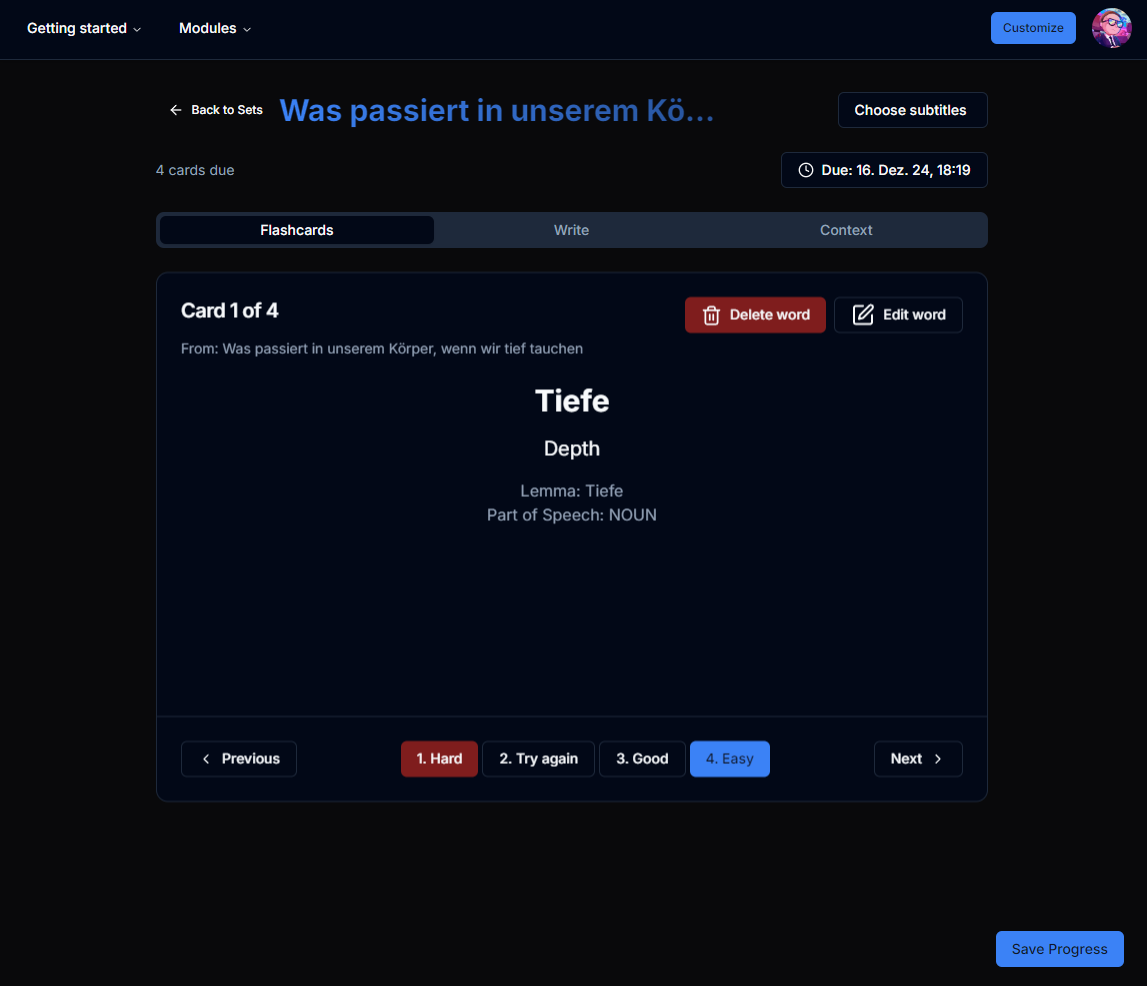
\includegraphics[width=1\textwidth]{IMAGE/FlashcardsLearn.png}
    \caption{Panel nauki fiszek}
    \label{fig:FlashcardsLearn}
\end{figure}

Panel nauki w aplikacji został zaprojektowany w oparciu o system fiszek oraz system powtórek oparty na algorytmie SRS (Space Repetition System). System fiszek umożliwia użytkownikom naukę nowych słów i zwrotów poprzez prezentowanie im kart z słowami i tłumaczeniami. Użytkownik może ocenić swoją znajomość danego słowa, co wpływa na to czy słowo przejdzie dalej czy nasze powtórki zostaną cofnięte \cite{mallett2012benefits}.

\subsection*{System powtórek SRS}

System SRS jest algorytmem, który optymalizuje proces nauki poprzez dostosowanie interwałów powtórek do indywidualnych potrzeb użytkownika. W praktyce oznacza to, że słowa, które użytkownik zna dobrze, będą pojawiać się rzadziej, natomiast te, które sprawiają trudności, będą powtarzane częściej. Dzięki temu użytkownik może efektywnie zarządzać swoim czasem nauki i skupić się na materiałach, które wymagają większej uwagi.

W panelu nauki użytkownik ma dostęp do różnych zestawów fiszek, które mogą być tworzone ręcznie lub generowane automatycznie na podstawie jego postępów i preferencji. Każda fiszka zawiera słowo lub zwrot w języku obcym oraz jego tłumaczenie lub definicję. Użytkownik może również edytowac fiszki, dodać tłumaczenie lub usuwać niepotrzebne lub niepoprawne informacje.

Dzięki zastosowaniu systemu SRS, panel nauki w aplikacji zapewnia skuteczną metodę nauki języka, która pozwala na osiąganie lepszych wyników w krótszym czasie. System automatycznie dostosowuje interwały powtórek na podstawie wyników użytkownika, co optymalizuje proces nauki bez konieczności ręcznej ingerencji \cite{mallett2012benefits}.

\subsection{Wirtualizacja List}
Wirtualizacja listy w aplikacjach internetowych to technika, która optymalizuje renderowanie długich list danych. Bez niej aplikacja renderuje wszystkie elementy listy na raz, co może prowadzić do problemów z wydajnością, zwłaszcza gdy lista jest duża. Virtualizacja polega na renderowaniu jedynie tych elementów, które aktualnie są widoczne w przeglądarce użytkownika, dzięki czemu zużycie zasobów jest minimalne, a aplikacja działa płynniej. Bez wirtualizacji listy, użytkownik mógłby doświadczać opóźnień w interakcji z interfejsem, tym większych im dłuższa lista danych przy 2 tysiącach wierszy opóźnienie stawało się uciążliwe ponieważ czekało sie pare sekund na reakcje interfejsu listy i pokazanie okna dodawania trudnych słów do systemu \cite{weng2004approach}.

\subsection*{Mechanizm działania wirtualizacji listy}
\begin{itemize}
    \item \textbf{Obserwacja widocznych elementów:} Komponent śledzi pozycję widoku użytkownika w liście. Renderowane są tylko te elementy, które mieszczą się w aktualnie widocznym obszarze (viewport) oraz kilka dodatkowych elementów „na zapas” wokół tego obszaru.
    \item \textbf{Renderowanie na żądanie:} Gdy użytkownik przewija listę, niewidoczne elementy są dynamicznie usuwane z DOM-u, a nowe – wczytywane na ich miejsce.
    \item \textbf{Stała wysokość elementów (lub szacowana):} Dla prawidłowego działania, komponent wirtualizujący często wymaga, aby elementy listy miały stałą lub przynajmniej przewidywalną wysokość. Dzięki temu może łatwo obliczać, które elementy powinny być aktualnie wyświetlane.
    \item \textbf{Oszczędność zasobów:} Dzięki renderowaniu tylko niewielkiej liczby elementów, zmniejsza się zużycie pamięci i obciążenie procesora, co prowadzi do szybszego działania aplikacji.
\end{itemize}
\subsection*{Przykładowy kod JavaScript}
Poniżej przedstawiono przykładowy kod tabeli Tanstack, który ilustruje operowanie na wierszach tabeli, takie jak śledzenie aktualnego do filmu wiersza napisów. Wiersz jest automatycznie przewijany do środkowego obszaru widocznego dla użytkownika, co ułatwia śledzenie napisów w czasie rzeczywistym. A index wiersza jest wybierany na podstawie czasu odtwarzania filmu, wybierany jest pierwszy wiersz na początek a potem przechodzi się na kolejny jeśli czas przekroczy wartość czasu w sekundach kolejnego wiersza.

\begin{lstlisting}[language=JavaScript, caption=Tablica Tanstack do wirtualizacji listy]
    export function DataTable<TData, TValue>({ captions, height }: { captions: Caption[], height: string }) {
        const [sorting, setSorting] = useState<SortingState>([]);
        const [currentIndex, setCurrentIndex] = useState<number>(0);
        const playedSeconds = useSelector((state: any) => state.subtitle.playedSeconds);
        const autoScrollEnabled = useSelector((state: any) => state.subtitle.autoScrollEnabled);
        const tableRef = useRef<TableVirtuosoHandle>(null);
        const table = useReactTable({
            data: captions,
            columns: columns,
            state: {
                sorting,
            },
            onSortingChange: setSorting,
            getCoreRowModel: getCoreRowModel(),
            getSortedRowModel: getSortedRowModel(),
        });
        const { rows } = table.getRowModel()
        useEffect(() => {
            if (rows.length > 0) {
                let newIndex = -1;
                for (let i = 0; i < rows.length; i++) {
                    const row = rows[i];
                    const startTime = row.original.start ?? 0;
                    const nextStartTime = rows[i + 1]?.original.start ?? Infinity;
                    if (playedSeconds >= startTime && playedSeconds < nextStartTime) {
                        newIndex = i;
                        break;
                    }
                }

                if (newIndex === -1) {
                    newIndex = 0;
                }
                setCurrentIndex(newIndex);
                if (autoScrollEnabled && tableRef.current && newIndex !== -1) {
                    tableRef.current.scrollToIndex({
                        index: newIndex,
                        align: "center",
                        behavior: "smooth",
                    });
                }
            }
        }, [playedSeconds, rows, autoScrollEnabled]);
\end{lstlisting}

\subsection*{Dlaczego React Virtuoso}
React Virtuoso jest biblioteką do wirtualizacji list, która znacznie upraszcza implementację tego mechanizmu w React. Automatycznie obsługuje:
\begin{itemize}
    \item \textbf{Przewijanie:} Zajmuje się wykrywaniem widocznych elementów, reagując na przewijanie użytkownika.
    \item \textbf{Niestandardowe wysokości elementów:} Obsługuje zarówno stałe, jak i zmienne wysokości elementów, co czyni go bardziej elastycznym.
    \item \textbf{Lazy loading:} Umożliwia ładowanie danych w locie, co jest kluczowe dla dużych list z elementami, które mogą być dynamicznie ładowane z serwera.
\end{itemize}

\subsection*{Zastosowania}
Virtualizacja listy jest szczególnie przydatna w przypadku:
\begin{itemize}
    \item \textbf{Długich list:} Kiedy lista zawiera setki lub tysiące elementów.
    \item \textbf{Aplikacji mobilnych:} Gdzie zasoby są ograniczone i każda optymalizacja wydajności jest istotna.
    \item \textbf{Interfejsów użytkownika z dużą ilością dynamicznych danych:} Takich jak portale społecznościowe, aplikacje e-commerce czy dashboardy.
\end{itemize}

\subsection*{Wady}
Mimo licznych zalet, wirtualizacja listy ma również pewne wady:
\begin{itemize}
    \item \textbf{Złożoność implementacji:} Wprowadzenie wirtualizacji może wymagać dodatkowego kodu i konfiguracji, co może zwiększyć złożoność projektu.
    \item \textbf{Problemy z dostępnością:} Renderowanie dynamiczne może wpływać na narzędzia do czytania ekranu i inne technologie wspomagające, co może utrudniać dostępność aplikacji.
\end{itemize}

Wykorzystanie React Virtuoso przyczyniło się do poprawy wydajności i płynności interfejsu użytkownika  aplikacji, co miało kluczowe znaczenie dla zadowolenia użytkowników i jakości doświadczenia użytkownika.

\section{Problemy implementacyjne}
\subsection{Wirtualizacja List}
Wirtualizacja listy w aplikacjach internetowych to technika, która optymalizuje renderowanie długich list danych. Bez niej aplikacja renderuje wszystkie elementy listy na raz, co może prowadzić do problemów z wydajnością, zwłaszcza gdy lista jest duża. Virtualizacja polega na renderowaniu jedynie tych elementów, które aktualnie są widoczne w przeglądarce użytkownika, dzięki czemu zużycie zasobów jest minimalne, a aplikacja działa płynniej. Bez wirtualizacji listy, użytkownik mógłby doświadczać opóźnień w interakcji z interfejsem, tym większych im dłuższa lista danych przy 2 tysiącach wierszy opóźnienie stawało się uciążliwe ponieważ czekało sie pare sekund na reakcje interfejsu listy i pokazanie okna dodawania trudnych słów do systemu.


\subsection*{Jak działa wirtualizacja listy}
\begin{itemize}
    \item \textbf{Obserwacja widocznych elementów:} Komponent śledzi pozycję widoku użytkownika w liście. Renderowane są tylko te elementy, które mieszczą się w aktualnie widocznym obszarze (viewport) oraz kilka dodatkowych elementów „na zapas” wokół tego obszaru.
    \item \textbf{Renderowanie na żądanie:} Gdy użytkownik przewija listę, niewidoczne elementy są dynamicznie usuwane z DOM-u, a nowe – wczytywane na ich miejsce.
    \item \textbf{Stała wysokość elementów (lub szacowana):} Dla prawidłowego działania, komponent wirtualizujący często wymaga, aby elementy listy miały stałą lub przynajmniej przewidywalną wysokość. Dzięki temu może łatwo obliczać, które elementy powinny być aktualnie wyświetlane.
    \item \textbf{Oszczędność zasobów:} Dzięki renderowaniu tylko niewielkiej liczby elementów, zmniejsza się zużycie pamięci i obciążenie procesora, co prowadzi do szybszego działania aplikacji.
\end{itemize}
\subsection*{Przykładowy kod JavaScript}
Poniżej przedstawiono przykładowy kod tabeli Tanstack, który ilustruje operowanie na wierszach tabeli, takie jak śledzenie aktualnego do filmu wiersza napisów. Wiersz jest automatycznie przewijany do środkowego obszaru widocznego dla użytkownika, co ułatwia śledzenie napisów w czasie rzeczywistym. A index wiersza jest wybierany na podstawie czasu odtwarzania filmu, wybierany jest pierwszy wiersz na początek a potem przechodzi się na kolejny jeśli czas przekroczy wartość czasu w sekundach kolejnego wiersza.

\begin{lstlisting}[language=JavaScript, caption=Tablica Tanstack do wirtualizacji listy]
    export function DataTable<TData, TValue>({ captions, height }: { captions: Caption[], height: string }) {
        const [sorting, setSorting] = useState<SortingState>([]);
        const [currentIndex, setCurrentIndex] = useState<number>(0);
        const playedSeconds = useSelector((state: any) => state.subtitle.playedSeconds);
        const autoScrollEnabled = useSelector((state: any) => state.subtitle.autoScrollEnabled);
        const tableRef = useRef<TableVirtuosoHandle>(null);
        const table = useReactTable({
            data: captions,
            columns: columns,
            state: {
                sorting,
            },
            onSortingChange: setSorting,
            getCoreRowModel: getCoreRowModel(),
            getSortedRowModel: getSortedRowModel(),
        });
        const { rows } = table.getRowModel()
        useEffect(() => {
            if (rows.length > 0) {
                let newIndex = -1;
                for (let i = 0; i < rows.length; i++) {
                    const row = rows[i];
                    const startTime = row.original.start ?? 0;
                    const nextStartTime = rows[i + 1]?.original.start ?? Infinity;
                    if (playedSeconds >= startTime && playedSeconds < nextStartTime) {
                        newIndex = i;
                        break;
                    }
                }

                if (newIndex === -1) {
                    newIndex = 0;
                }
                setCurrentIndex(newIndex);
                if (autoScrollEnabled && tableRef.current && newIndex !== -1) {
                    tableRef.current.scrollToIndex({
                        index: newIndex,
                        align: "center",
                        behavior: "smooth",
                    });
                }
            }
        }, [playedSeconds, rows, autoScrollEnabled]);
\end{lstlisting}

\subsection*{Dlaczego React Virtuoso}
React Virtuoso jest biblioteką do wirtualizacji list, która znacznie upraszcza implementację tego mechanizmu w React. Automatycznie obsługuje:
\begin{itemize}
    \item \textbf{Przewijanie:} Zajmuje się wykrywaniem widocznych elementów, reagując na przewijanie użytkownika.
    \item \textbf{Niestandardowe wysokości elementów:} Obsługuje zarówno stałe, jak i zmienne wysokości elementów, co czyni go bardziej elastycznym.
    \item \textbf{Lazy loading:} Umożliwia ładowanie danych w locie, co jest kluczowe dla dużych list z elementami, które mogą być dynamicznie ładowane z serwera.
\end{itemize}

\subsection*{Zastosowania}
Virtualizacja listy jest szczególnie przydatna w przypadku:
\begin{itemize}
    \item \textbf{Długich list:} Kiedy lista zawiera setki lub tysiące elementów.
    \item \textbf{Aplikacji mobilnych:} Gdzie zasoby są ograniczone i każda optymalizacja wydajności jest istotna.
    \item \textbf{Interfejsów użytkownika z dużą ilością dynamicznych danych:} Takich jak portale społecznościowe, aplikacje e-commerce czy dashboardy.
\end{itemize}

\subsection*{Wady}
Mimo licznych zalet, wirtualizacja listy ma również pewne wady:
\begin{itemize}
    \item \textbf{Złożoność implementacji:} Wprowadzenie wirtualizacji może wymagać dodatkowego kodu i konfiguracji, co może zwiększyć złożoność projektu.
    \item \textbf{Problemy z dostępnością:} Renderowanie dynamiczne może wpływać na narzędzia do czytania ekranu i inne technologie wspomagające, co może utrudniać dostępność aplikacji.
\end{itemize}

Wykorzystanie React Virtuoso przyczyniło się do poprawy wydajności i płynności interfejsu użytkownika  aplikacji, co miało kluczowe znaczenie dla zadowolenia użytkowników i jakości doświadczenia użytkownika.

\subsection{Przetwarzanie języka naturalnego (NLP)}
W pracy inżynierskiej zastosowano techniki lematyzacji oraz oznaczania części mowy (POS tagging) w ramach przetwarzania języka naturalnego (NLP). Obie te techniki odegrały kluczową rolę w analizie tekstu i umożliwiły bardziej precyzyjne przetwarzanie danych z napisów, przy zapisywaniu wybranych przez użytkownika słów do nauki, lub przy wyświetlaniu częstości występowania słów w napisach \cite{NLPforNLP}.

\subsection*{Lematyzacja}
Proces lematyzacji polega na sprowadzaniu różnych form gramatycznych wyrazów do ich podstawowej formy, zwanej lematem. Dzięki temu możliwe jest ujednolicenie wyrazów, które w zależności od kontekstu występują w różnych odmianach gramatycznych. Przykładowo, formy takie jak "chodzę", "chodził" czy "chodziliśmy" są sprowadzane do podstawowej formy "chodzić". Umożliwia to bardziej spójne analizowanie tekstów i wyciąganie wniosków na temat ich zawartości, np. poprzez obliczanie częstotliwości występowania poszczególnych słów \cite{NLPforNLP}.

\subsection*{POS Tagging (oznaczanie części mowy)}
Drugą techniką było oznaczanie części mowy, czyli przypisywanie każdemu słowu w tekście odpowiedniej etykiety gramatycznej (rzeczownik, czasownik, przymiotnik itd.)  \cite{NLPforNLP}. Dzięki temu możliwe było lepsze zrozumienie struktury zdań oraz funkcji słów w kontekście. Oznaczanie części mowy okazało się kluczowe w procesie analizy tekstu, umożliwiając podział słów na kategorie zależne od ich funkcji gramatycznej. W przyszłości może to być przydatne do tworzenia funkcji umożliwiających użytkownikom wybór nauki określonych kategorii słów, takich jak czasowniki czy przymiotniki itd.









\chapter{Podsumowanie}
% Projekt aplikacji webowej wspomagającej naukę języków obcych za pomocą filmów i seriali stanowi nowoczesne i proste narzędzie edukacyjne. Integracja funkcji nauki oraz oglądania treści wideo w jednym miejscu nie tylko upraszcza proces nauki, ale także eliminuje potrzebę korzystania z wielu różnych aplikacji i narzędzi. To podejście pozwala na maksymalne wykorzystanie czasu użytkownika, zwiększając efektywność nauki poprzez dostęp do materiałów w naturalnym kontekście językowym.

\section{Wnioski}

Projekt aplikacji webowej wspomagającej naukę języków obcych za pomocą filmów i seriali stanowi nowoczesne narzędzie edukacyjne. Integracja funkcji nauki i oglądania w jednym miejscu ułatwia użytkownikom proces przyswajania wiedzy, eliminując konieczność korzystania z dodatkowych aplikacji. Aplikacja umożliwia przechowywanie trudnych słów, śledzenie postępów oraz korzystanie z panelu nauki, co czyni ją wszechstronnym narzędziem wspomagającym naukę języków. Ponadto, interaktywne podejście do nauki poprzez kontekstualne użycie języka w filmach i serialach zwiększa zaangażowanie użytkowników i poprawia efektywność nauki. Dzięki temu użytkownicy mogą uczyć się w sposób bardziej naturalny i przyjemny, co sprzyja długotrwałemu zapamiętywaniu nowych informacji.

Celem pracy inżynierskiej było stworzenie aplikacji, która pozwoli użytkownikom na naukę języka w sposób bardziej naturalny, efektywny i dostosowany do indywidualnych potrzeb. Cel ten został zrealizowany poprzez zaprojektowanie systemu, który integruje naukę języka z oglądaniem treści wideo, co czyni proces edukacyjny bardziej dynamicznym i przyjaznym dla użytkownika.



\section{Kierunki dalszego rozwoju}
% Dalszy rozwój aplikacji może obejmować dodanie nowych funkcji, takich jak integracja z innymi platformami streamingowymi, rozwój panelu nauki o dodatkowe metody jak, gry edukacyjne czy interaktywne ćwiczenia. Dodatkowe modele NLP do innych języków również mogą okazać się przydatne, umożliwiając naukę mniej popularnych języków takich jak chiński gdzie problemem jest brak przerw między słowami co utrudnia aplikacji dodawanie trudnych słów do bazy danych. Ponadto, wprowadzenie funkcji społecznościowych, takich jak fora dyskusyjne czy możliwość współpracy z innymi użytkownikami, mogłoby zwiększyć zaangażowanie i motywację do nauki.

Dalszy rozwój aplikacji powinien obejmować rozbudowę jej funkcjonalności oraz poszerzenie zakresu dostępnych możliwości. W pierwszej kolejności wskazane jest wprowadzenie integracji z popularnymi platformami streamingowymi, co pozwoli na korzystanie z różnorodnych materiałów wideo bez konieczności dodatkowej konfiguracji.

Panel nauki może zostać wzbogacony o nowe metody wspierające proces edukacyjny, takie jak gry edukacyjne, interaktywne ćwiczenia czy testy wiedzy. Rozszerzenie aplikacji o obsługę większej ilości języków mogłoby zostać zrealizowane poprzez wdrożenie zaawansowanych modeli przetwarzania języka naturalnego (NLP), które umożliwią naukę mniej popularnych języków.

Wprowadzenie funkcji społecznościowych, takich jak fora dyskusyjne, grupy nauki czy możliwość współpracy między użytkownikami, stanowiłoby kolejny krok w rozwoju aplikacji. Takie rozwiązania mogłyby sprzyjać budowaniu motywacji oraz zwiększać zaangażowanie użytkowników w proces nauki.

Rozszerzenie funkcjonalności aplikacji o mechanizmy personalizacji, takie jak algorytmy rekomendujące treści dostosowane do poziomu i zainteresowań użytkownika, mogłoby znacząco wpłynąć na efektywność nauczania. Dodanie audio do treści w procesie nauki mogłoby stanowić dodatkowy element wspierający naukę, umożliwiając użytkownikom lepsze zrozumienie wymowy i intonacji w naturalnym kontekście językowym.


	
	% Bibliografia - musi byc
	% Bibliography - must exist
	\bibliografia
	
	% Strony koncowe - mozna zakomentowac, jesli zbedne
	% Additional pages - comment out if not needed
	
	\clearpage
	% Spis rysunków
	\clearpage
	\listoffigures
	% Spis tabel
	\clearpage
	\listoftables
	
	\clearpage
	\lstlistoflistings
	
	
\end{document}
%%%%%%%%%%%%%%%%%%%%%%%%%%%%%%%%%%%%%%%%%%%%%%%%%%%%%%%%%%%%%%%%%%%%%%%%%%%

\end{lstlisting}
Po zakończeniu ustawiania i napisaniu streszczenia należy rozwinąć katalog \texttt{Chapters} i otworzyć plik \texttt{main.tex} gdzie można umieścić czy napisać poszczególne rozdziały pracy. Autor zaleca pisane rozdziałów w osobnych plikach ponieważ rozdziały napisane w jednym pliku będą  bardzo duże i trudne do zarządzania. Chcąc dodać nowy rozdział należy utworzyć nowy plik w katalogu \texttt{Chapters} po czym w pliku \texttt{main.tex} i dodać go w odpowiednim miejscu. Trzeba pamiętać o tym że pliki umieszczone są w kolejności w jakiej będą prezentowane w pracy. W pliku \texttt{main.tex} żeby dodać nowy rozdział trzeba użyć poleceń \texttt{\textbackslash chapters\{Nazwa Rozdziału\} i \textbackslash input\{ścieżka do pliku\}}. 

\begin{lstlisting}[caption={Tworzenie nowych rozdziałów}, label=lst:Tworzenie nowych rozdziałów]

% Rozdzialy zaczynaja sie od "chapter"
\chapter{Introduction}
% Praca podzielona na mniejsze pliki wlaczane za pomoca input
\input{Chapters/Introduction}

\end{lstlisting}
\section{Rysunki}\label{sec:grafika}

Rysunki \LaTeX\ umieszczamy w otoczeniu \texttt{"figure"} i za pomocą komendy \texttt{\textbackslash includegraphics} Otoczenie to pozwala na dodanie podpisu \texttt{(caption)} i znacznika \texttt{(label)} dzięki któremu potem można się do nich odnosić za pomocą komendy \texttt{\textbackslash ref\{sec:nazwa znacznika\}}.
Oto przykład wstawiania rysunku do dokumentu.
\begin{lstlisting}[caption={Kod wstawiający prosty rysunek}, label=lst:Kod wstawiający prosty rysunek]
\begin{figure}[!hb]
    \includegraphics{obraz.jpg}
    \caption{Podpis do obrazu}
    \label{fig:moja-etykieta}
\end{figure}
\end{lstlisting}
Rysunki można przenosić jeśli nie trafił tam gdzie powinien. Trzeba wtedy zmienić pozycje rysunku w przykładzie \texttt{[!hb]} na jedną z niżej wymiennych opcji:
\begin{itemize}
\item [--] \textbf{h} - umieść rysunek tutaj (here), jeśli to możliwe,
\item [--] \textbf{t} - umieść rysunek na górze strony (top),
\item [--] \textbf{b} - umieść rysunek na dole strony (bottom).
\item [--] \textbf{p} - umieść rysunek na osobnej stronie (page).
\item [--] \textbf{!} - ignoruj większość zasad pozycjonowania i sugeruje, aby naruszyć pewne domyślne zasady.
\end{itemize}
Możesz również łączyć te opcje, na przykład [ht] oznacza "tutaj" lub na górze strony.
Dodatkowe obcję których można użyć w otoczeniu \texttt{figure}
\begin{itemize}
\item scale\\
Odpowiada za rozmiar, wprowadź [scale=2.0]. Ta liczba może przyjąć dowolną wartość; liczba między 0 a 1 zmniejszy grafikę, a liczba ujemna odwróci ją,

\item angle\\
 Kąt jest podawany w stopniach i zgodnie z ruchem wskazówek zegara. Grafika jest obracana wokół swojego pochodzenia,
\item width\\
Umożliwia ustawienie szerokości obrazu,
\item height\\
Daje możliwość zmiany wysokości obrazu.
\end{itemize}

\begin{figure}[!ht]
	\centering 
 \includegraphics[width=0.5\linewidth]{IMAGE/Strona tytułowa pracy.png}
	\caption{Strona tytułowa pracy}
	\label{rys:Strona tytułowa pracy}
\end{figure}
Poniżej znajdziemy kod poprawinie wstawionego obrazu z przykładu \ref{rys:Strona tytułowa pracy}
\begin{lstlisting}[caption={Kod poprawnie wstawionego obrazu}, label=lst:Kod poprawnie wstawionego obrazu]
	\begin{figure}[!h]
		\includegraphics[width=0.5\linewidth]{IMAGE/Strona tytulowa pracy.png}
		\caption{Strona tytulowa pracy}
		\label{rys:Strona tytulowa pracy}
	\end{figure}
\end{lstlisting}


\section{Odwołania do literatury}
Zarządzanie bibliografią w \LaTeX\ odbywa się automatycznie. Nie trzeba się przejmować dodawanie czy usuwaniem pozycji z bibliografii. Dzięki wcześniejszym ustawieniom bibliografia sortuje się według ustawionego schematu.W bibliografii pojawiają się tylko te przypisy, do których odwołania istnieją w treści.
Odniesienia do literatury tworzy się za pomocą komendy \texttt{\textbackslash cite\{id\}} w którym podaje się znacznik przypisany danej pozycji. Noty bibliograficzne powinny znajdować się w osobnym pliku \href{./Dyplom.bib}{\texttt{Dyplom.bib}}. Każda zmiana pliku bibliografii wymaga jego rekompilacji.
W szablonie używany jest program biber który w \overleaflink uruchamia się automatyczne przy zmianie bibliografii\\
Oto przykładowe odwołanie do literatury ~\cite{fowler2009} \texttt{\textbackslash cite\{fowler2009\}}.\\
Wszystkie odwołania robi się praktycznie tak samo. Chcąc odnieść się do kilku pozycji jednocześnie, trzeba ich znaczniki wpisać po przecinku ~\cite{kopka2003guide,fowler2009} \texttt{\textbackslash cite\{kopka2003guide,fowler2009\}}.\\
Można też odnieść się do konkretnej strony ~\cite[s.~38]{kopka2003guide} \texttt{\textbackslash cite[s.~38]\{kopka2003guide\}}.\\
Znak tyldy (\keys{\textasciitilde{}}) przed wywołaniem \texttt{cite} ,,skleja'' odnośnik z~poprzedzającym je słowem za pomocą tak zwanej ,,twardej'' spacji.

Ułatwieniem może być to, że serwisy takie jak Google Scholar, Mendeley czy Zoteor pozwalają na pobranie cytowania w postaci BibTeX.

\section{Tabele}\label{sec:tabel}

Aby stworzyć prostą tabelę w \LaTeX\, możesz skorzystać z otoczenia \texttt{table}. 
Przykład tworzenia prostej tabeli w \LaTeX\

\begin{lstlisting}[caption={Kod prostej tabeli}, label=lst:Kod prostej tabeli]
	\begin{table}[h]
		\centering
		\begin{tabular}{p{2.5cm}c|l}
			Przyklad  &   Przyklad           &   Przyklad\\\hline\hline
			Przyklad  &   Przyklad           &   Przyklad\\\hline
			Przyklad  &   Przyklad           &   Przyklad \\\hline
			Przyklad  &   Przyklad           &   Przyklad\\\hline
			Przyklad  &   Przyklad           &   Przyklad\\\hline
			Przyklad  &   Przyklad           &   Przyklad
		\end{tabular}
		\caption{\label{tab:Prosta tabela}Prosta tabela}
	\end{table}
\end{lstlisting}

W przykładzie \ref{lst:Kod prostej tabeli} został przedstawiony prosty kod tworzący table mieszczący się w otoczeniu \texttt{table} i \texttt{tabular}. Pozycje tabeli ustawiamy jak w przypadku rysunków \ref{sec:grafika} natomiast jeśli chodzi o otoczenie \texttt{tabular} przy którym specyfikacja kolumn określa liczbę i format kolumn tabeli. Liczbę kolumn i~ułożenie w~nich tekstu określa się jako argumenty polecenia \texttt{tabular}:
\begin{itemize}
	\item l -- dosunięcie do lewej,
	\item r -- dosunięcie do prawej,
	\item c -- centrowanie,
	\item p -- styl akapitowy z~szerokością określoną parametrem.
\end{itemize}
Wpisując zawartość każdej komórki tabeli, oddzielając je znakiem \textbf{"\&"}. Każdy wiersz kończ \textbf{"\textbackslash"}.
Komenda \texttt{\textbackslash hline} służy do dodawania poziomych linii w tabelach. Jest to polecenie, które umieszczasz wewnątrz środowiska tabeli.
Kończąc tabele należy pamiętać aby nadać jej tytuł ora etykietę.
Tabela poniżej jest przykładem wygenerowanej tabeli z lisingui \ref{lst:Kod prostej tabeli}.
\begin{table}[H]
 \centering
  \begin{tabular}{p{2.5cm}c|l}
    Przykład  &   Przykład           &   Przykład\\\hline\hline
    Przykład  &   Przykład           &   Przykład\\\hline
    Przykład  &   Przykład           &   Przykład \\\hline
    Przykład  &   Przykład           &   Przykład\\\hline
    Przykład  &   Przykład           &   Przykład\\\hline
    Przykład  &   Przykład           &   Przykład
  \end{tabular}
 \caption{\label{tab:Tabela wygenerowana kodem z listingu 12}Tabela wygenerowana kodem z listingu 12}
\end{table}
Tabele należą do najtrudniejszym elementem do wprowadzenia w~
\LaTeX{u} ze względu na nagromadzenie znaczników. Dlatego warto rozważyć edytowanie tabel za pomocą dedykowanego edytora takiego jak \href{https://www.tablesgenerator.com}{TablesGenerator} w których tworzymy tabele graficznie a edytor automatycznie generuje nam z tego kod \LaTeX\ który wystarczy wstawić w interesującym nas miejscu.

\section{Wzory}\label{sec:Wzory}
Wzory matematyczne w \LaTeX\ zapisuje się za pomocą poleceń. Proste i popularne symbole są łatwe do zapamiętania.
Natomiast, jeśli potrzebne są bardziej złożone wzory lub mniej powszechnie używane symbole, warto sięgnąć po dokumentację, dostępną na przykład na stronach takich jak \href{https://www.overleaf.com/learn/latex/Mathematical_expressions}{Overleaf}. Można  skorzystać z~edytorów równań dostępnych online, takich jak:
\begin{itemize}
    \item \href{https://latex.codecogs.com/eqneditor/editor.php}{CodeCogs}
    \item \href{https://www.latex4technics.com/}{Latex4technics}
\end{itemize}
Ich zaletami są natychmiastowe generowane wzory.
Wzory Matematyczne w \LaTeX\ piszemy w środowisku \texttt{equation} pisane wzory w tym środowisku są w tryb wyłączony (display) czyli występują w osobnej linii. Istnieje również możliwość pisania wzorów matematycznych w Linii teku za pomocą znaków dolara. 
Poniżej znajduje się kilka przykładów zapisania wzorów. W pierwszym przykładzie użyto dodatkowej opcji otoczenia \texttt{equation} która wyłącza numerowanie poprzez dodanie do otoczenia *. Warto zapoznać się z dokumentacją dotyczącą wzorów na stronie internetowej \cite{overleaf}

\begin{equation*}
    r = \sqrt{r_x^2 + r_y^2}
\end{equation*}

\begin{equation}
    \frac{dx}{dx} = 1
\end{equation}

\begin{equation}
    \frac{d}{dx} \ln x = \frac{1}{x}
\end{equation}

\begin{equation}
    y = \varphi  (y^\prime)x + \psi(y^\prime)
\end{equation}

\begin{gather}
 \begin{bmatrix} \Phi_{11} & \Phi_{12} \\ \Phi_{21} & \Phi_{22} \end{bmatrix}
 =
 \frac{1}{\det(X)}
  \begin{bmatrix}
   X_{22} Y_{11} - X_{12} Y_{21} &
   X_{22} Y_{12} - X_{12} Y_{22} \\
   X_{11} Y_{21} - X_{21} Y_{11} &
   X_{11} Y_{22} - X_{21} Y_{12} 
   \end{bmatrix}
\end{gather}

\clearpage
\section{Kody Żródłowe}
Pakiet umożliwiający wstawianie kodów źródłowych z różnych języków programowania do dokumentu to \texttt{listingu}. Więcej informacji można znaleźć na przykład w~dokumentacji \href{https://www.overleaf.com/learn/latex/code_listing}{Overleaf} Poniżej znajdziesz krótką instrukcję używania pakietu listingu:\\

Wstaw kod źródłowy do dokumentu, używając otoczenia lstlisting.
\begin{lstlisting}[caption={Przykladowy kod}, label=lst:przyklad]
\begin{lstlisting}[caption={Przykladowy kod}, label=lst:przyklad]
public class HelloWorld {
    public static void main(String[] args) {
        System.out.println("Hello, World!");
    }
}
end{lstlisting}
\end{lstlisting}

\begin{lstlisting}[language=Python,
    caption={Prosty program w~języku python},
    label={lst:hellopy}]
#!/usr/bin/env python
# -*- coding: utf-8 -*-
"""Simple world of hello.
"""

import sys

def main():
    """The one and only function"""
    fib = lambda n: reduce(lambda x, n: [x[1], x[0]+x[1]], range(n), [0, 1])[0]
    try:
        print(fib(int(sys.argv[1])))
    except:
        print("Hello World!")

if __name__ == "__main__":
    main()
\end{lstlisting}
Kody źródłowe można też dołączać w zewnętrznych plikach i załączać automatycznie.
Istnieje możliwość wskazania zakresu lini które pojawią się w dokumencie listing \ref{lst:Kod} ma automatycznie ustawiany podpis na podstawie nazwy pliku.


\lstinputlisting[language=C,
    firstnumber=33,
    firstline=33,
    lastline=50,
    caption=Kod pobrany z zewnętrzego pliku,
    label={lst:Kod}]{Kod.c}

\section{Grafy, schematy, rysunki techniczne}

Pakiet \texttt{tikz} w \LaTeX\ umożliwia rysowanie grafiki wektorowej i tworzenie różnych rodzajów ilustracji, w tym diagramów, grafów, schematów, czy rysunków technicznych.
W tworzeniu schematów może pomóc internetowy edytor \href{https://tikzmaker.com}{\texttt{Tikzmaker}} który generuje kod na podstawie grafiki. \\
Poniżej znajdziesz podstawową instrukcję dotyczącą korzystania z otoczenia \texttt{tikzpicture}:\\
Umieść otoczenie tikzpicture wewnątrz środowiska \texttt{figure}, jeśli chcesz mieć możliwość dodania podpisu i etykiety. Poniżej w listingu 17 został przedstawiony przykład rysujący funkcje kwadratową z rysunku \ref{fig:Funkcja kwadratowa}.

\begin{lstlisting}[caption={Kod rysujący funkcje kwadratową}, label=lst:Kod rysujący funkcje kwadratową]
\begin{figure}
	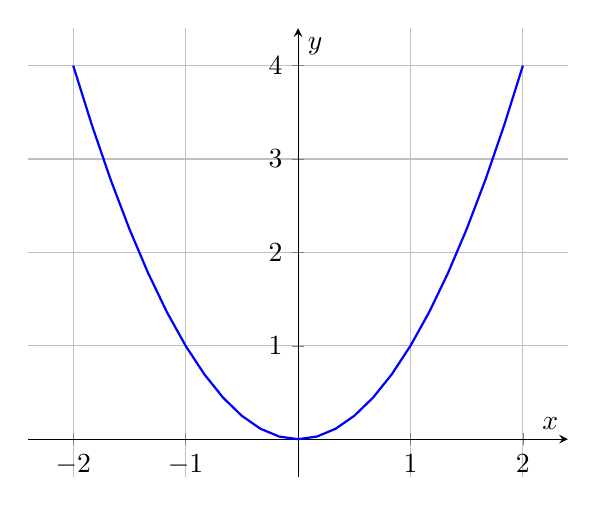
\begin{tikzpicture}
		\begin{axis}[
			xlabel=$x$,
			ylabel=$y$,
			grid=both,
			axis lines=middle,
			enlargelimits,
			]
			\addplot[domain=-2:2, color=blue, thick]{x^2};
		\end{axis}
	\end{tikzpicture}
	\caption{Funkcja kwadratowa}
	\label{fig:Funkcja kwadratowa}
\end{figure}
\end{lstlisting}


\begin{figure}[!h]
	\centering
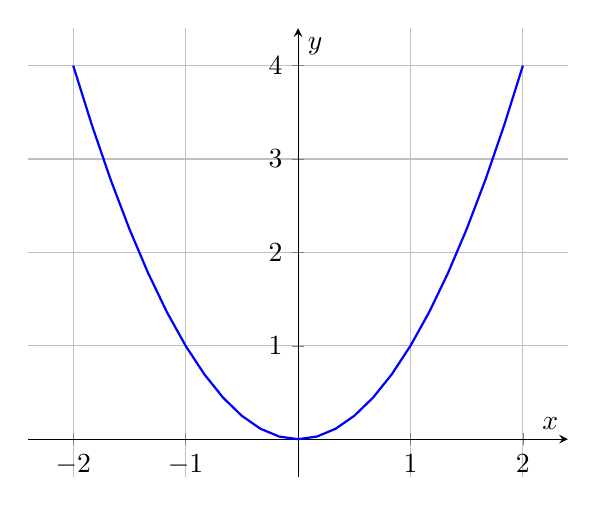
\begin{tikzpicture}
	\begin{axis}[
		xlabel=$x$,
		ylabel=$y$,
		grid=both,
		axis lines=middle,
		enlargelimits,
		]
		\addplot[domain=-2:2, color=blue, thick]{x^2};
	\end{axis}
\end{tikzpicture}
\caption{Funkcja kwadratowa z lisingu 16}
\label{fig:Funkcja kwadratowa}
\end{figure}
Szablon umożliwia tworzenie wykresów poprzez wczytywanie danych z plików. Dane do wykresów powinny być umieszczone w folderze \texttt{charts}. Wykres \ref{fig:multiplot} został stworzy poprzez wczytanie danych z pliku za pomocą kodu podanego w listingu \ref{lst:Wykrez wczytany z pliku}
\begin{figure}[!hb]
	\centering
	\begin{tikzpicture}
		% First subplot
		\begin{axis}[
			ybar,
			xlabel={Category},
			ylabel={Value},
			bar width=0.5cm,
			symbolic x coords={A, B, C},
			xtick=data,
			]
			\addplot table [x index=0, y index=1] {charts/bar_data1.txt};
			\addlegendentry{Plot 2}
			\addplot table [x index=0, y index=1] {charts/bar_data3.txt};
			\addlegendentry{Plot 2}
		\end{axis}
	\end{tikzpicture}
	\caption{Przykład wykresu wczytywanego z pliku}
	\label{fig:multiplot}
\end{figure}
\clearpage
\begin{lstlisting}[caption={Wykrez wczytany z pliku}, label=lst:Wykrez wczytany z pliku]
	\begin{figure}[!hb]
		\centering
		\begin{tikzpicture}
			% First subplot
			\begin{axis}[
				ybar,
				xlabel={Category},
				ylabel={Value},
				bar width=0.5cm,
				symbolic x coords={A, B, C},
				xtick=data,
				]
				\addplot table [x index=0, y index=1] {charts/bar_data1.txt};
				\addlegendentry{Plot 2}
				\addplot table [x index=0, y index=1] {charts/bar_data3.txt};
				\addlegendentry{Plot 2}
			\end{tikzpicture}
			\caption{Multiplot Example}
			\label{fig:multiplot}
		\end{figure}
	\end{lstlisting}
Dokumentacja \texttt{TikZ} jest obszerna i zawiera wiele przykładów. Warto ją przeczytać, aby poznać pełne możliwości pakietu. TikZ oferuje wiele zaawansowanych funkcji, a dokładne dostosowania można znaleźć w jego dokumentacji.
\href{https://tikz.dev}{tikz.dev}\\

Pakiet \texttt{circuitikz} umożliwia rysowanie obwodów elektrycznych. Oto podstawowe instrukcje dotyczące korzystania z circuitikz:
Rozpoczęcie Środowiska circuitikz:
Umieść otoczenie circuitikz wewnątrz otoczenia \texttt{figure}, jeśli chcesz mieć możliwość dodania podpisu i etykiety.
Poniżej w lisnigu \ref{fig:funkcja} został przedstawiony kod rysujący schemat przedstawiony w schemacie \ref{fig:schemat}
\begin{lstlisting}[caption={Schemat użycia circuitikz}, label=lst:Schemat użycia circuitikz ]
\begin{figure}[H]
	\centering
	\begin{circuitikz}[american voltages]
		\draw
		(0,0) to [short, *-] (6,0)
		to [V, l_=$\mathrm{j}{\omega}_m \underline{\psi}^s_R$] (6,2) 
		to [R, l_=$R_R$] (6,4) 
		to [short, i_=$\underline{i}^s_R$] (5,4) 
		(0,0) to [open, v^>=$\underline{u}^s_s$] (0,4) 
		to [short, *- ,i=$\underline{i}^s_s$] (1,4) 
		to [R, l=$R_s$] (3,4)
		to [L, l=$L_{\sigma}$] (5,4) 
		to [short, i_=$\underline{i}^s_M$] (5,3) 
		to [L, l_=$L_M$] (5,0); 
	\end{circuitikz}
	\caption{Schemat}
	\label{fig:funkcja}
\end{figure}
\end{lstlisting}
\begin{figure}[H]
    \centering
    \begin{circuitikz}[american voltages]
        \draw
        (0,0) to [short, *-] (6,0)
        to [V, l_=$\mathrm{j}{\omega}_m \underline{\psi}^s_R$] (6,2) 
        to [R, l_=$R_R$] (6,4) 
        to [short, i_=$\underline{i}^s_R$] (5,4) 
        (0,0) to [open, v^>=$\underline{u}^s_s$] (0,4) 
        to [short, *- ,i=$\underline{i}^s_s$] (1,4) 
        to [R, l=$R_s$] (3,4)
        to [L, l=$L_{\sigma}$] (5,4) 
        to [short, i_=$\underline{i}^s_M$] (5,3) 
        to [L, l_=$L_M$] (5,0); 
    \end{circuitikz}
    \caption{Schemat}
    \label{fig:schemat}
\end{figure}
Dokumentacja:
Pełna dokumentacja circuitikz zawiera obszerny spis elementów i dostępnych opcji. Można ją znaleźć na 
\href{https://texdoc.org/serve/circuitikzmanual.pdf/0}{Circuitikz Dokumentacja}\\



\section{Dodatki}

\subsection{Podstawowe style tekstu}
\begin{itemize}
    \item \textbf{tekst wytłuszczony} \textbackslash textbf{\{tekst wytłuszczony\}},
    \item \textit{tekst pochylony} \textbackslash textit{\{tekst pochylony\}},

    \item \texttt{tekst maszynowy} \textbackslash texttt{\{tekst maszynowy\}},
     
    \item \underline{tekst podkreślony} \textbackslash underline{\{tekst podkreślony\}},
    \item W pracy zostało stworzone makro które zmienia kolor tekstu maszynowego na szary \maszynowy{tekst maszynowy} \textbackslash maszynowy{\{tekst maszynowy\}}.
\end{itemize}
\subsection{Wiszące znaki}
W polskiej tradycji literackiej pojedyncze znaki, takie jak a, i, o, u, w, z, nie powinny występować na końcu linii. Aby uniknąć tego problemu i połączyć tę literę z następującym słowem, używa się znaku tyldy (\keys{\textasciitilde{}}).

Na koniec pisania pracy najlepiej zamienić wszystkie ciągi znaków przy pomocy ,,znajdź i~zamień'' z \keys{\SPACE, znak, \SPACE} na \keys{\SPACE, znak, \textasciitilde{}}.

\subsection{Wyliczenia}
Tworzenie wyliczeń w \LaTeX\ odbywa się za pomocą otoczenia \texttt{itemize} w którym każdy kolejny punkt dodajemy za pomocą komędy \texttt{\textbackslash item} . Poniżej znajduje się przykład użycia otoczenia \texttt{itemize}
\begin{itemize}
    \item standardową "kropke",
    \item[--] myślnik.
\end{itemize}
Podczas używania warto poznać zasady interpunkcji w wyliczeniach z którymi można zapoznać się w artykule \cite{ekorekta24} lub w blogu \cite{contentwriter}.
\subsection{Akronimy i~symbole}
Szablon używa pakietu \texttt{glossaries} do zarządzania akronimami i~symbolami. Listę tych elementów należy przygotować w~pliku \href{./glossary.tex}{glossary.tex}, zgodnie z~pokazanym szablonem \textbackslash newacronym\{PO\}\{\{PO\}\{Politechnika Opolska\}.

\subsection{Ozdobniki graficzne w~opisie oprogramowania}
Szablon wczytuje pakiet pozwalający na wyróżnienie w~tekście informacji o~skrótach klawiszowych, poruszaniu się po menu programu i~ścieżki plików. Aby użyć tego pakietu należy zastosować komendę \texttt{\textbackslash keys{\{Nazwa klawisza\}}}.\\
W tekście można wyróżnić skróty klawiszowe, takie jak na przykład:
\begin{itemize} 
 	\item \keys{\Alt, F4}, \keys{\ctrl, \Alt, \del},
    \item \keys{A, a, B, b, C, c, 1, 2, 3, PgUp},
    \item \keys{\Space} \keys{\SPACE},
    \item \keys{\backspace} \keys{\del} \keys{\backdel},
    \item \keys{\return} \keys{\enter},
    \item \keys{\shift} \keys{\capslock}.
\end{itemize}

\subsection{Kompilator lokalny}\label{sec:kompilator_lokalny}
Problemem darmowej wersji Overeleaf jest to, że zapewnia krótki czas kompilowania nie dłuższy niż 1 minute. W przypadku gdy praca jest skomplikowana czas ten może zostać przekroczony i  nie wygeneruje nam pliku wynikowego. Rozwiązaniem tego problemu jest zainstalowanie na własnym komputerze kompilatora lokalnego. Aby to poprawnie zrobić najperw należy zainstalować \href{https://www.ghostscript.com}{\texttt{Ghostscript}}. Ghostscript to interpreter języka PostScript i Portable Document Format (PDF), służący do przetwarzania i wyświetlania plików w tych formatach. Po udanym zainstalowaniu Ghostscript należy zainstalować \href{https://miktex.org/}{\texttt{MiKTeX}} który jest dystrybucją oprogramowania do składu tekstu opartą na \TeX\ / \LaTeX\ . Ostatnim wymaganym programem jest edytor tekstu który możemy wybrać według własnych preferencji. Najczęsciej używane edytory tekstu to:
\begin{itemize}
	\item[--]\href{https://www.tug.org/texworks/}{\texttt{TeXworks}},
	\item[--]\href{https://www.texstudio.org}{\texttt{Texstudio}},
	\item[--]\href{https://www.winedt.com}{\texttt{WinEdt}},
	\item[--]\href{https://code.visualstudio.com}{\texttt{Visual Studio Code}} do którego należy dodać rozszerzenie \texttt{\LaTeX\ Workshop}
\end{itemize}
Dzięki dodaniu na początku dokument tzw. komentarzy magicznych (ang.magic comments) lub dyrektywy \TeX\ (ang. \TeX\ directives) edytory tekstu automatycznie pobierają informacje jakiego kompilatora powinny użyć, w jakim kodowaniu jest dokument i włączają sprawdzanie pisowni w języku polskim.
\begin{lstlisting}[caption={Dyrektywy \TeX\ }, label=lst:Komentarze magiczne]
% !TEX program = xelatex
% !TeX encoding = utf8
% !TeX spellcheck = pl-PL
\end{lstlisting}

\subsection{Oświadczenia i wnioski}
 Wyborze plików po lewej stronie również są wrzucone oświadczenia i wnioski które mogą się przydać podczas składania pracy.
 
 \section{Prezentacja}
Podczas tworzenia szablonu do pracy dyplomowej został stworzony szablon do prezentacji dyplomowej. Wygląd prezentacji zostało oparty na podstaiwe zatwierdzonego szablonu przygotowanego w Microsoft PowerPoint. Do tworzenia prezentacji w \LaTeX\ istnieje osobna klasa dokumenty \texttt{beamer}. Używając w ten sposób klasy tworzy nam się prezentacja w rozdzielczości 4:3 dzięki argumentowi \texttt{[aspectratio=169]} jesteśmy wstanie zmienic rozdzielczość naszej prezentacji na 19:4. W stworzonej przez autora prezentacji istnieje kastomizowany slajd tytułowy w którym automatycznie zostają umieszczone tytuł, podtytuł, autor, oraz instutucja podane w odpowiedznich miejscach. 
\begin{lstlisting}[caption={Prsonalizacja prezentacji}, label=lst:Personalizacja prezentacji]
\title{Szablon prezentacji \LaTeX}
\subtitle{Podtytul}
\author[Autor]{Autor}
\institute{Instytucja}
\end{lstlisting}

Nowe slajdy w prezentacji tworzy się za pomocą otoczenia \texttt{frame} w lizingu \ref{lst:Tworzenie pustego slajdu w prezentacji} przykład tworzenia nowego slajdu
\begin{lstlisting}[caption={Tworzenie pustego slajdu w prezentacji}, label=lst:Tworzenie pustego slajdu w prezentacji]
\begin{frame}
	\frametitle{Tytuł slajdu} 
	Tresc slajdu
	\end{frame}
\end{lstlisting}
W miejscu \texttt{frametitle} należy wpisać tytuł slajdu. W następnym wierszu umieszczamu treść naszego slajdu i całość zamykamy otoczeniem \texttt{frame} 
Prezentacja posiada pakiety takie same jak szablon do pracy dyplomowej dzięki czemu tworzenie nowych slajdów i dodawanie do nich takich elementów jak wzory, tabele czy rysunki odbywa się w ten sam sposób jak przedstawiony w podrozdziałach \ref{sec:Wzory}. \ref{sec:grafika}, \ref{sec:tabel}. Jednak należy pamiętać aby dodać listing do prezentacji trzeba użyć dodatkowego argumentu \texttt{[fragile]} przy tworzeniu nowego slajdu.
\begin{lstlisting}[caption={Slajd z kodem źródłowym}, label=lst:Slajd z kodem źródłowym]
\begin{frame}[fragile]
\frametitle{Prezentacja w \LaTeX\ } 
Fragment kodu
\end{lstlisting}
 W prezentacjach \LaTeX\ jest możliwość automatycznego podziału długich zawartości slajdów na kilka stron za pomocą opcji \texttt{allowframebreaks}. Jest szczególnie przydatna, gdy zawartość jednego slajdu nie mieści się na ekranie i potrzebny jest automatyczny podział na kolejne strony. Ta opcja pomaga w utrzymaniu czytelności i przejrzystości prezentacji.
\begin{figure}[!ht]
\centering 
\includegraphics[width=1\linewidth]{IMAGE/Strona tytułowa prezentacji.png}
\caption{Strona tytułowa prezentacji}
\label{rys:Strona tytułowa prezentacji}
\end{figure}


